\documentclass[compress]{beamer}
\mode<presentation>
\usetheme{Warsaw}
\usecolortheme{seagull}

%\useoutertheme[subsection=false]{smoothbars}

%\usepackage{stackengine}
%\setbeamertemplate{caption}{\raggedright\insertcaption\par}
\setbeamertemplate{caption}{\insertcaption} 
%\usepackage{caption}
%\usepackage{pgffor}

\usepackage{fancybox}
\usepackage{minibox}

%\usepackage{tcolorbox}
\usepackage{empheq}


%% ====================================== graphics

\usepackage{pgfplots}
\pgfplotsset{width=10cm,compat=1.9}
%\usepgfplotslibrary{external}
%\tikzexternalize
 \usepackage{pgfplotstable}

%\definecolor{markercolor}{RGB}{.49, 1, .63}
\definecolor{markercolor}{RGB}{124.9, 255, 160.65}

\pgfplotsset{
tick label style={font=\scriptsize},
label style={font=\scriptsize},
legend style={font=\scriptsize},
title style={font=\footnotesize}
}

%% ===========================================
\usepackage{stmaryrd}

\usepackage{amsmath,amsfonts,amsthm}

% for FD grid tikz
\usepackage{tikz,amssymb}
\usetikzlibrary{calc}
\newcommand\bound{10}

\usepackage{slopetri}

\useoutertheme{infolines}
\useinnertheme{rectangles}
\usepackage{hhline}
\setbeamercovered{dynamic}

\usepackage{soul}

\usepackage{array}
\usepackage{mathrsfs}
\usepackage[utf8]{inputenc}
\usepackage{listings}
\usepackage{mathtools}
\usepackage{bm}
\usepackage{cancel}


\usepackage{graphicx}
\usepackage{subfig}
\makeatletter
\let\@@magyar@captionfix\relax
\makeatother

\usepackage{color}

\usepackage{bibentry}
\nobibliography*

\theoremstyle{plain}

\renewcommand{\hat}{\widehat}
\renewcommand{\tilde}{\widetilde}

%% d in integrand
\newcommand*\diff[1]{\mathop{}\!{\mathrm{d}#1}}
\newcommand{\diag}[1]{{\rm diag}\LRp{#1}}
\newcommand{\td}[2]{\frac{{\rm d}#1}{{\rm d}{\rm #2}}}
\newcommand{\pd}[2]{\frac{\partial#1}{\partial#2}}
\newcommand{\nor}[1]{\left\| #1 \right\|}
\newcommand{\LRp}[1]{\left( #1 \right)}
\newcommand{\LRs}[1]{\left[ #1 \right]}
\newcommand{\LRa}[1]{\left\langle #1 \right\rangle}
\newcommand{\LRb}[1]{\left| #1 \right|}
\newcommand{\LRc}[1]{\left\{ #1 \right\}}
\newcommand{\LRceil}[1]{\left\lceil #1 \right\rceil}
\newcommand{\LRu}[1]{\left. #1 \right|}
\newcommand{\pdn}[3]{\frac{\partial^{#3}#1}{\partial#2^{#3}}}
\newcommand{\Grad} {\ensuremath{\nabla}}
\newcommand{\jump}[1] {\ensuremath{\llbracket#1\rrbracket}}
\newcommand{\avg}[1] {\ensuremath{\LRc{\!\{#1\}\!}}}

\graphicspath{{./figs/}}

\renewcommand{\note}[1]{\textcolor{red}{{#1}}}
%\renewcommand{\note}[1]{{\color{blue}{#1}}}


% removes nav symbols
\beamertemplatenavigationsymbolsempty
%\setbeamertemplate{caption}{\raggedright\insertcaption\par}

% defines newblock as null, giving compile issues otherwise
\let\newblock\relax 


\title[Entropy stable DG]{Entropy stable schemes based on high order modal discontinuous Galerkin formulations}
\date[4/3/19]{Finite Elements in Flow, Chicago, Illinois\\April 3, 2019}
\author[J.\ Chan]{Jesse Chan\\ {\footnotesize with Lucas Wilcox (NPS), DCDR Fernandez, Mark Carpenter (NASA Langley)}}
\institute[Rice CAAM]{\inst{1}Department of Computational and Applied Mathematics}

\begin{document}
\makeatletter
\@addtoreset{subfigure}{framenumber}% subfigure counter resets every frame
\makeatother

\begin{frame}
\maketitle
\end{frame}

%% =================================================


\frame{
\frametitle{High order methods typically unstable for nonlinear PDEs}
\setcounter{subfigure}{0}
\vspace{-1em}
\begin{figure}
\begin{overprint}
\centering
\foreach \id in {1,2,3,4}{%
\only<\id>{
\captionsetup[subfloat]{width=.45\textwidth, justification=centering}
\subfloat[Inviscid Burgers' solution]{%[$N = 7, K = 8$ (aligned mesh)]{
\makebox[.425\textwidth]{\includegraphics[width=.4\textwidth]{figs/burgersStable_\id.png}}}%
\hspace{1em}%
\subfloat[8th order DG]{ %[$N = 7, K = 9$ (non-aligned mesh)]{
\makebox[.425\textwidth]{\includegraphics[width=.4\textwidth]{figs/burgersUnstable_\id.png}}}
} % only
} % foreach 
\end{overprint}
\end{figure}
\vspace{-.25em}
\begin{itemize}
\item High order methods tend to blow up for under-resolved solutions (shocks, turbulence), sensitive to discretization.  
\vspace{.25em}
\item Instability: \note{quadrature error} + loss of the discrete \note{chain rule} in space.  
\end{itemize}
}


\frame{
\frametitle{Entropy stability for nonlinear problems uses the chain rule}
\vspace{-.5em}
\begin{itemize}
\item Generalizes energy stability to \note{nonlinear} systems of conservation laws (Burgers', shallow water, compressible Euler, MHD).  
\[
\pd{\bm{u}}{t} + \pd{\bm{f}(\bm{u})}{x} = 0 \qquad x \in [-1,1].
\]
\item Continuous entropy inequality: given a scalar convex \note{entropy} function $S(\bm{u})$ and ``entropy potential'' $\psi(\bm{u})$, 
\begin{align*}
&\int_{-1}^1 \bm{v}^T\LRp{\pd{\bm{u}}{t} + \pd{\bm{f}(\bm{u})}{x}} = 0, \qquad \boxed{\bm{v} = \pd{S}{\bm{u}}} \\
&\Longrightarrow \pd{}{t}\int_{-1}^1 S(\bm{u}) + \LRu{\LRp{\bm{v}^T\bm{f}(\bm{u}) - \psi(\bm{u})}}_{-1}^1 \leq 0.
\end{align*}
%\vspace{.01em}
\item Proof of entropy inequality relies on \note{chain rule}, {integration by parts}.  
\end{itemize}

\let\thefootnote\relax\footnotetext{\tiny Continuous entropy stability: Hughes et al.\ 1986, Zakerzadeh/May, Fernandez/Nguyen/Peraire, Williams, \ldots}
}




\section{Entropy stable nodal DG and summation-by-parts}


\frame[noframenumbering]{
\frametitle{Talk outline}
\tableofcontents
}

\frame[noframenumbering]{
\frametitle{Talk outline}
\tableofcontents[currentsection]
}

\frame{
\frametitle{Nodal DG, summation-by-parts (SBP), flux differencing}
\setcounter{subfigure}{0}
\vspace{-1em}
\begin{figure}
\centering
\subfloat{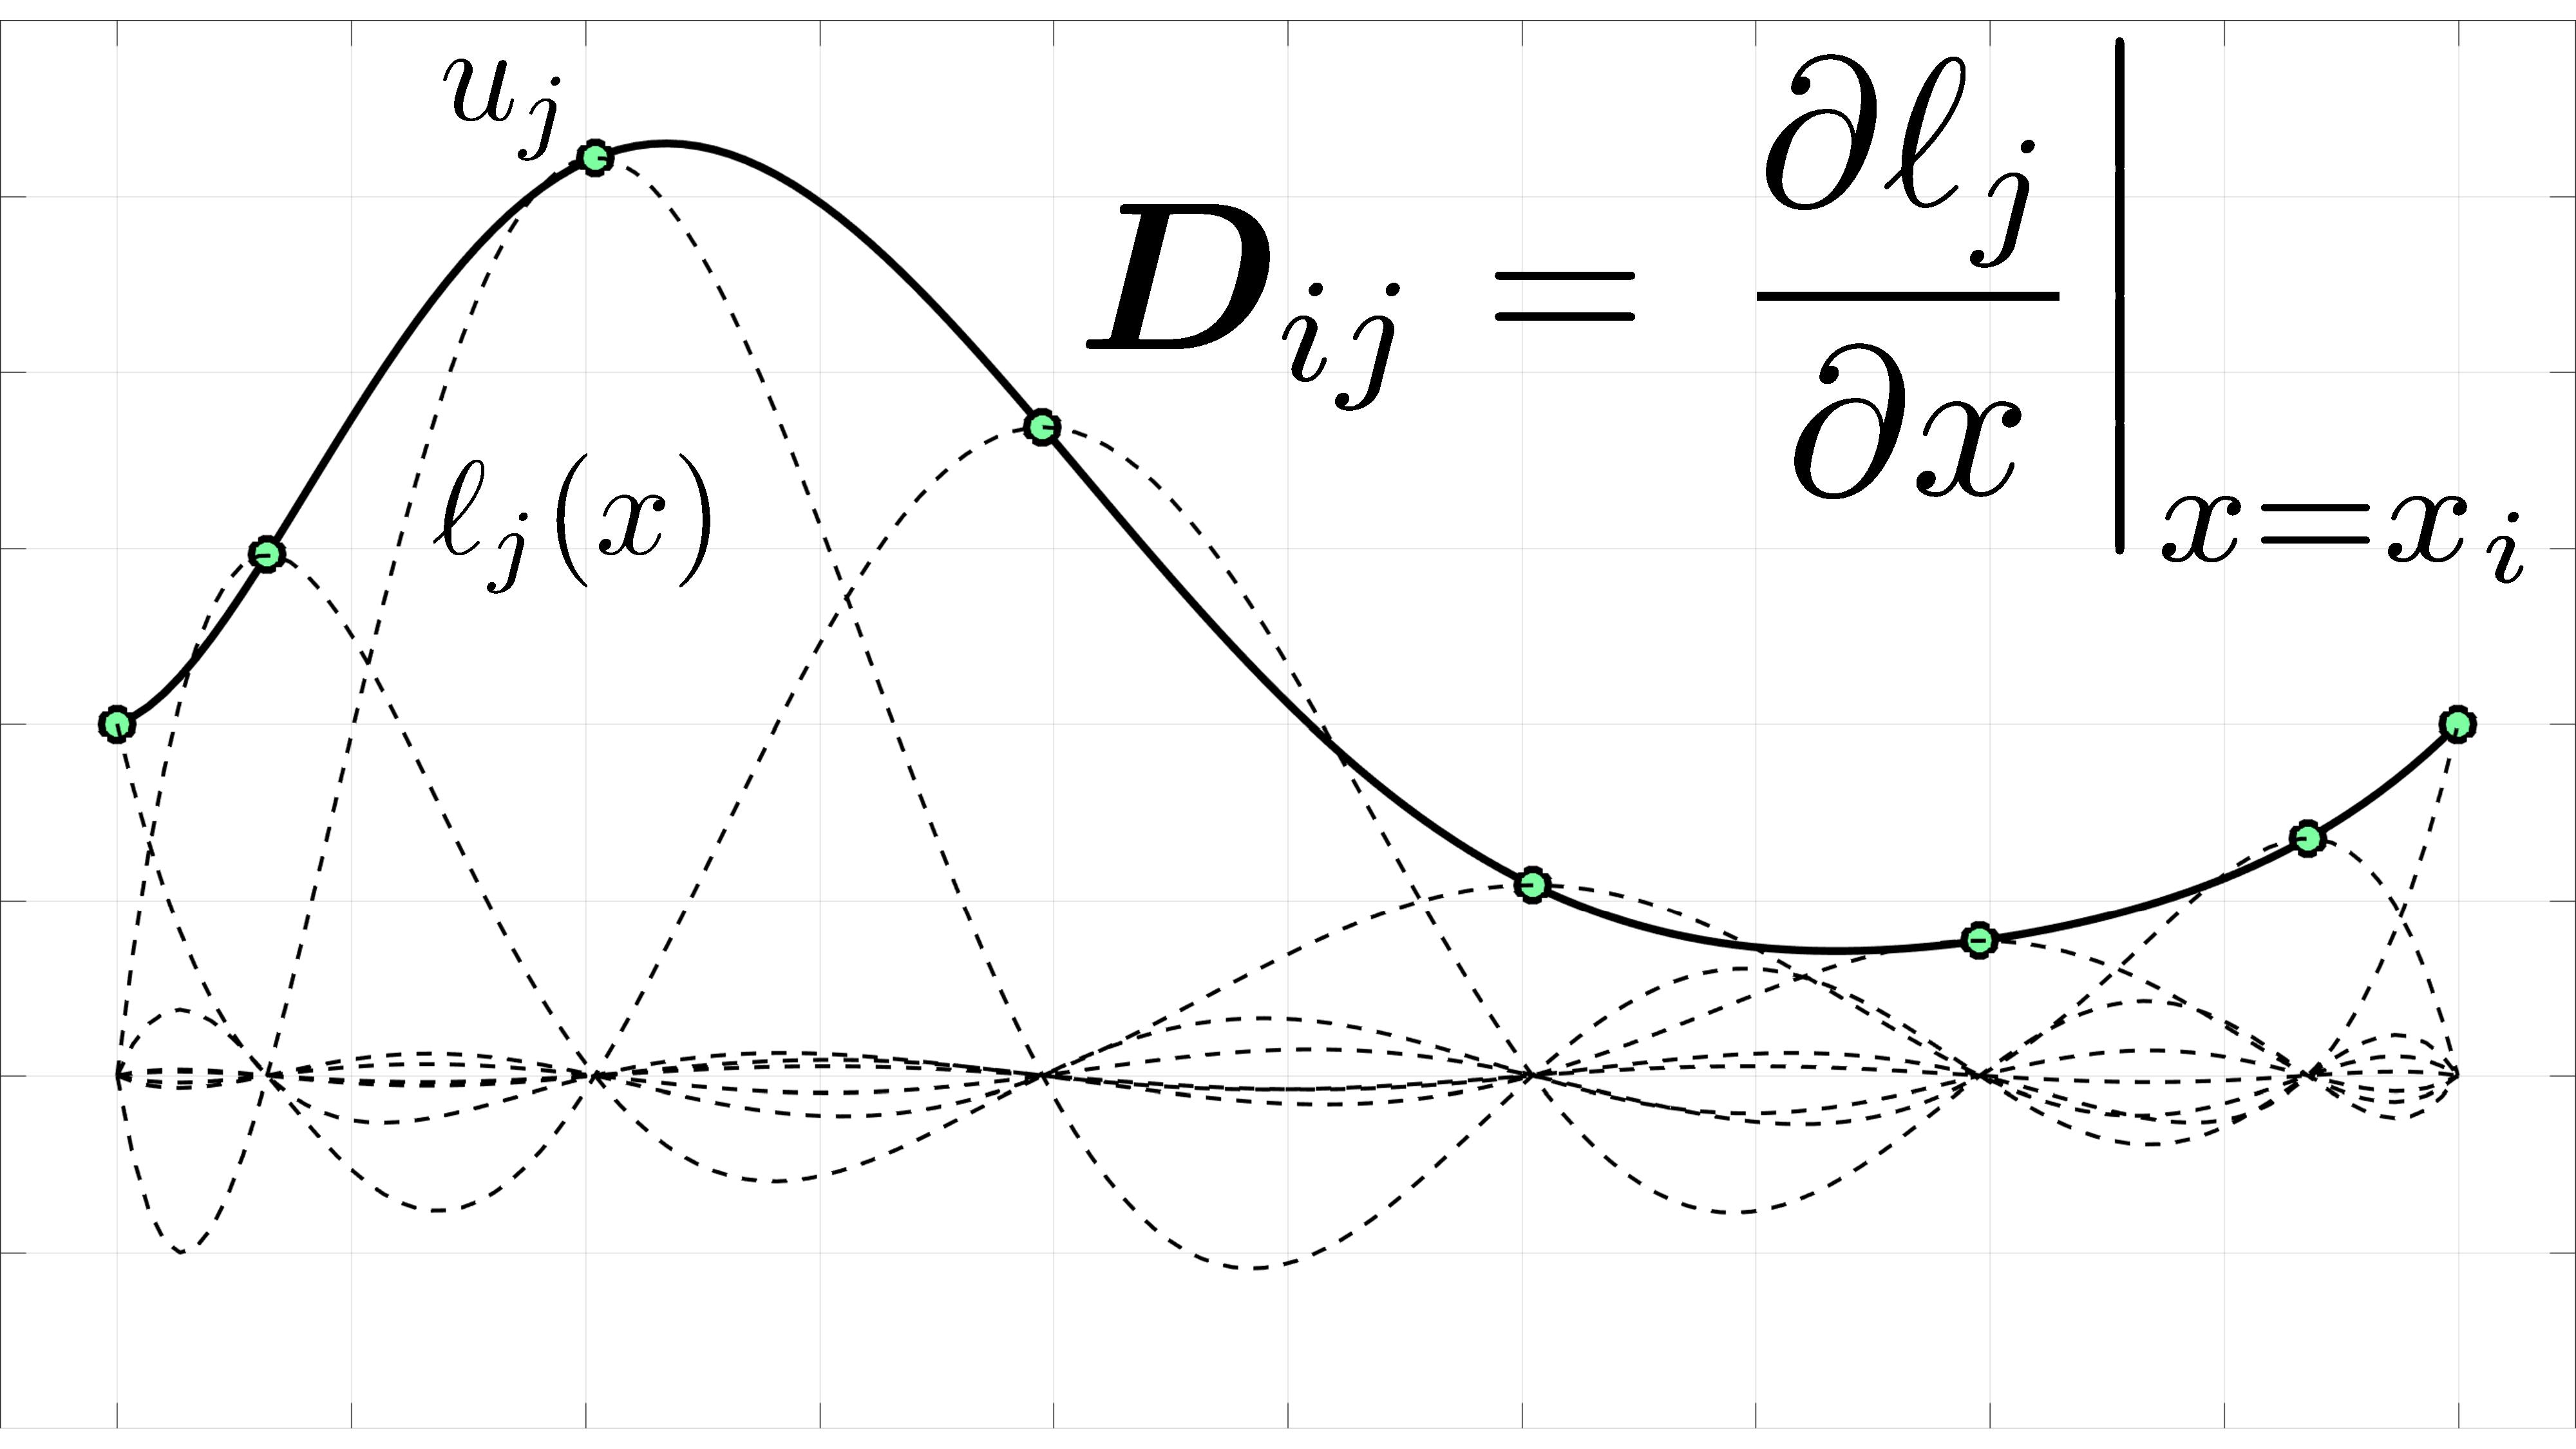
\includegraphics[width=.33\textwidth]{figs/gll1Dsbp.pdf}}
\hspace{2.5em}
\subfloat{\raisebox{.5em}{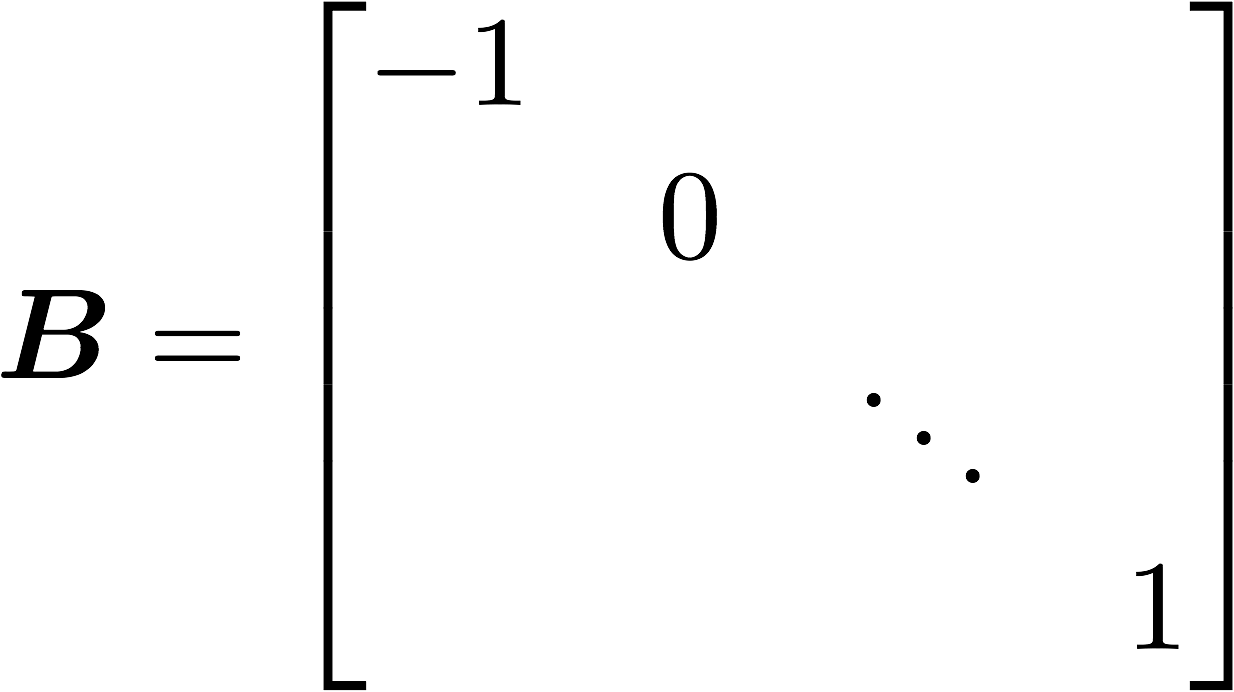
\includegraphics[width=.30\textwidth]{figs/B_SBP.png}}}
\end{figure}
\vspace{-.25em}
\begin{itemize}
\item Gauss-Lobatto nodes mimic \note{integration by parts} algebraically % using differentiation matrix $\bm{D}$, diagonal (lumped) mass matrix $\bm{M}$, boundary matrix $\bm{B}$
\[
\boxed{\bm{Q} = \bm{B} - \bm{Q}^T,} \qquad \bm{Q} = \bm{M}\bm{D}, \qquad \bm{M} \text{ diagonal mass matrix}.
\]
\item<2-> Nodal ``collocation'' over a single element:
\[
\bm{M}\td{\bm{u}}{t} + \bm{Q}\bm{f}(\bm{u}) = 0 \quad  \Longrightarrow \quad \bm{M}_{ii}\td{\bm{u}_i}{t} + \sum_{j} \bm{Q}_{ij} \bm{f}\LRp{\bm{u}_j} = 0.
\]
\item<3-> Let $\bm{f}_S(\bm{u}_i,\bm{u}_j) = \frac{1}{2}\LRp{\bm{f}(\bm{u}_i)+\bm{f}(\bm{u}_j)} = \LRp{\bm{F}_S}_{ij}$.  Collocation equiv.\ to
\[
\bm{M}_{ii}\td{\bm{u}_i}{t} + \sum_{j} \bm{Q}_{ij} \note{2\bm{f}_S\LRp{\bm{u}_i,\bm{u}_j}} = 0 \quad \Longrightarrow \quad \boxed{\bm{M}\td{\bm{u}}{t} + 2\LRp{\bm{Q}\circ\note{\bm{F}_S}}\bm{1} = 0.}
\]
\end{itemize}

%\let\thefootnote\relax\footnotetext{\tiny Gassner (2013). \textit{A skew-symmetric DG-SEM discretization and its relation to SBP-SAT finite difference methods.}}
%\let\thefootnote\relax\footnotetext{\tiny Figure courtesy of David C.\ Del Rey Fernandez.}
%\let\thefootnote\relax\footnotetext{\tiny Fisher and Carpenter (2013). \textit{High-order ES finite difference schemes for nonlinear conservation laws: Finite domains.} }
%\let\thefootnote\relax\footnotetext{\tiny Gassner, Winters, and Kopriva (2016). \textit{Split form nodal DG schemes with SBP property for the comp.\ Euler equations.}}
%\let\thefootnote\relax\footnotetext{\tiny Chen and Shu (2017). \textit{ES high order DG methods with suitable quadrature rules for hyperbolic conservation laws.}}
%\let\thefootnote\relax\footnotetext{\tiny Crean, Hicken, et al.\ (2018). \textit{Entropy-stable SBP discretization of the Euler equations on general curved elements.}}
}



\frame{
\frametitle{Entropy stable schemes: a brief derivation}

\begin{itemize}
\item<1-> DG: derive local formulation (one element) with interface flux $\bm{f}^*$
\begin{overlayarea}{\textwidth}{.17\textheight}
\vspace{-1em}
\begin{align*}
\only<1>{\bm{M}\td{\bm{u}}{t} + 2\LRp{\bm{Q}\circ\bm{F}_S}\bm{1} = 0}
\only<2>{\bm{M}\td{\bm{u}}{t} + \underbrace{\LRp{\LRp{\note{\bm{Q}-\bm{Q}^T}}\circ\bm{F}_S}\bm{1}}_{\text{SBP property}} + \LRp{\note{\bm{B}}\circ\bm{F}_S}\bm{1} = 0}
\only<3>{\bm{M}\td{\bm{u}}{t} + \LRp{\LRp{\bm{Q}-\bm{Q}^T}\circ\bm{F}_S}\bm{1} + \underbrace{\note{\bm{B}\bm{f}(\bm{u})}}_{\LRp{\bm{F}_S}_{ii} = \bm{f}(\bm{u}_i) \text{ + diagonal } \bm{B}}  = 0.}
\only<4>{\bm{M}\td{\bm{u}}{t} + \LRp{\LRp{\bm{Q}-\bm{Q}^T}\circ\bm{F}_S}\bm{1} + \underbrace{\note{\bm{B}\bm{f}^*}}_{\text{Numerical flux}} = 0.  }
\only<5->{\bm{M}\td{\bm{u}}{t} + \LRp{\LRp{\bm{Q}-\bm{Q}^T}\circ\bm{F}_S}\bm{1} + \bm{B}\bm{f}^* = 0.  }
\end{align*}
\end{overlayarea}
\item<6-> Trick: use Tadmor's entropy conservative numerical flux for $\bm{f}_S, \bm{f}^*$
\begin{align*}
\bm{f}_S(\bm{u},\bm{u}) &= \bm{f}(\bm{u}), \qquad \text{(consistency)} \\
\bm{f}_S(\bm{u},\bm{v}) &= \bm{f}_S(\bm{v},\bm{u}),\qquad \text{(symmetry)} \\
\LRp{\bm{v}_L - \bm{v}_R}^T \bm{f}_S\LRp{\bm{u}_L,\bm{u}_R} &= \psi_L - \psi_R, \qquad \text{(conservation)}.
\end{align*}
\item<7-> Proof of entropy \note{conservation}: multiply by $\bm{v}^T$
\begin{overlayarea}{\textwidth}{.175\textheight}
\[
\hspace*{-1em}
\only<1-7>{\bm{v}^T\bm{M}\td{\bm{u}}{t} + \bm{v}^T\LRp{\LRp{\bm{Q}-\bm{Q}^T}\circ\bm{F}_S}\bm{1} + \bm{v}^T\bm{B}\bm{f}^* = 0.}
\only<8>{\bm{1}^T\bm{M}\td{S(\bm{u})}{t} + \sum_{ij} \bm{Q}_{ij} \note{\LRp{\bm{v}_i-\bm{v}_j}^T \bm{f}_S\LRp{\bm{u}_i,\bm{u}_j}} + \bm{v}^T\bm{B}\bm{f}^* = 0.}
\only<9>{\bm{1}^T\bm{M}\td{S(\bm{u})}{t} + \sum_{ij} \bm{Q}_{ij} \note{\LRp{\psi(\bm{u}_i)-\psi(\bm{u}_j)}} + \bm{v}^T\bm{B}\bm{f}^* = 0.}
\only<10>{\bm{1}^T\bm{M}\td{S(\bm{u})}{t} + \note{\bm{\psi}^T\bm{Q}\bm{1} - \bm{1}^T\bm{Q}\bm{\psi}} + \bm{v}^T\bm{B}\bm{f}^* = 0.}
\only<11>{\bm{1}^T\bm{M}\td{S(\bm{u})}{t} + \bm{1}^T\bm{B}\LRp{\bm{v}^T\bm{f}^* - \bm{\psi}}  = 0.}
\]
\end{overlayarea}
\end{itemize}
\let\thefootnote\relax\footnotetext{\tiny Tadmor, Eitan (1987), Gassner, Winters, and Kopriva (2016).}
}


\frame{
\frametitle{Benefits of entropy stability (conservation)}
\vspace{-.5em}
\begin{figure}
\centering
\begin{overlayarea}{\textwidth}{.45\textheight}
\only<1>{
\subfloat[Entropy conservative flux, $T = .3$]{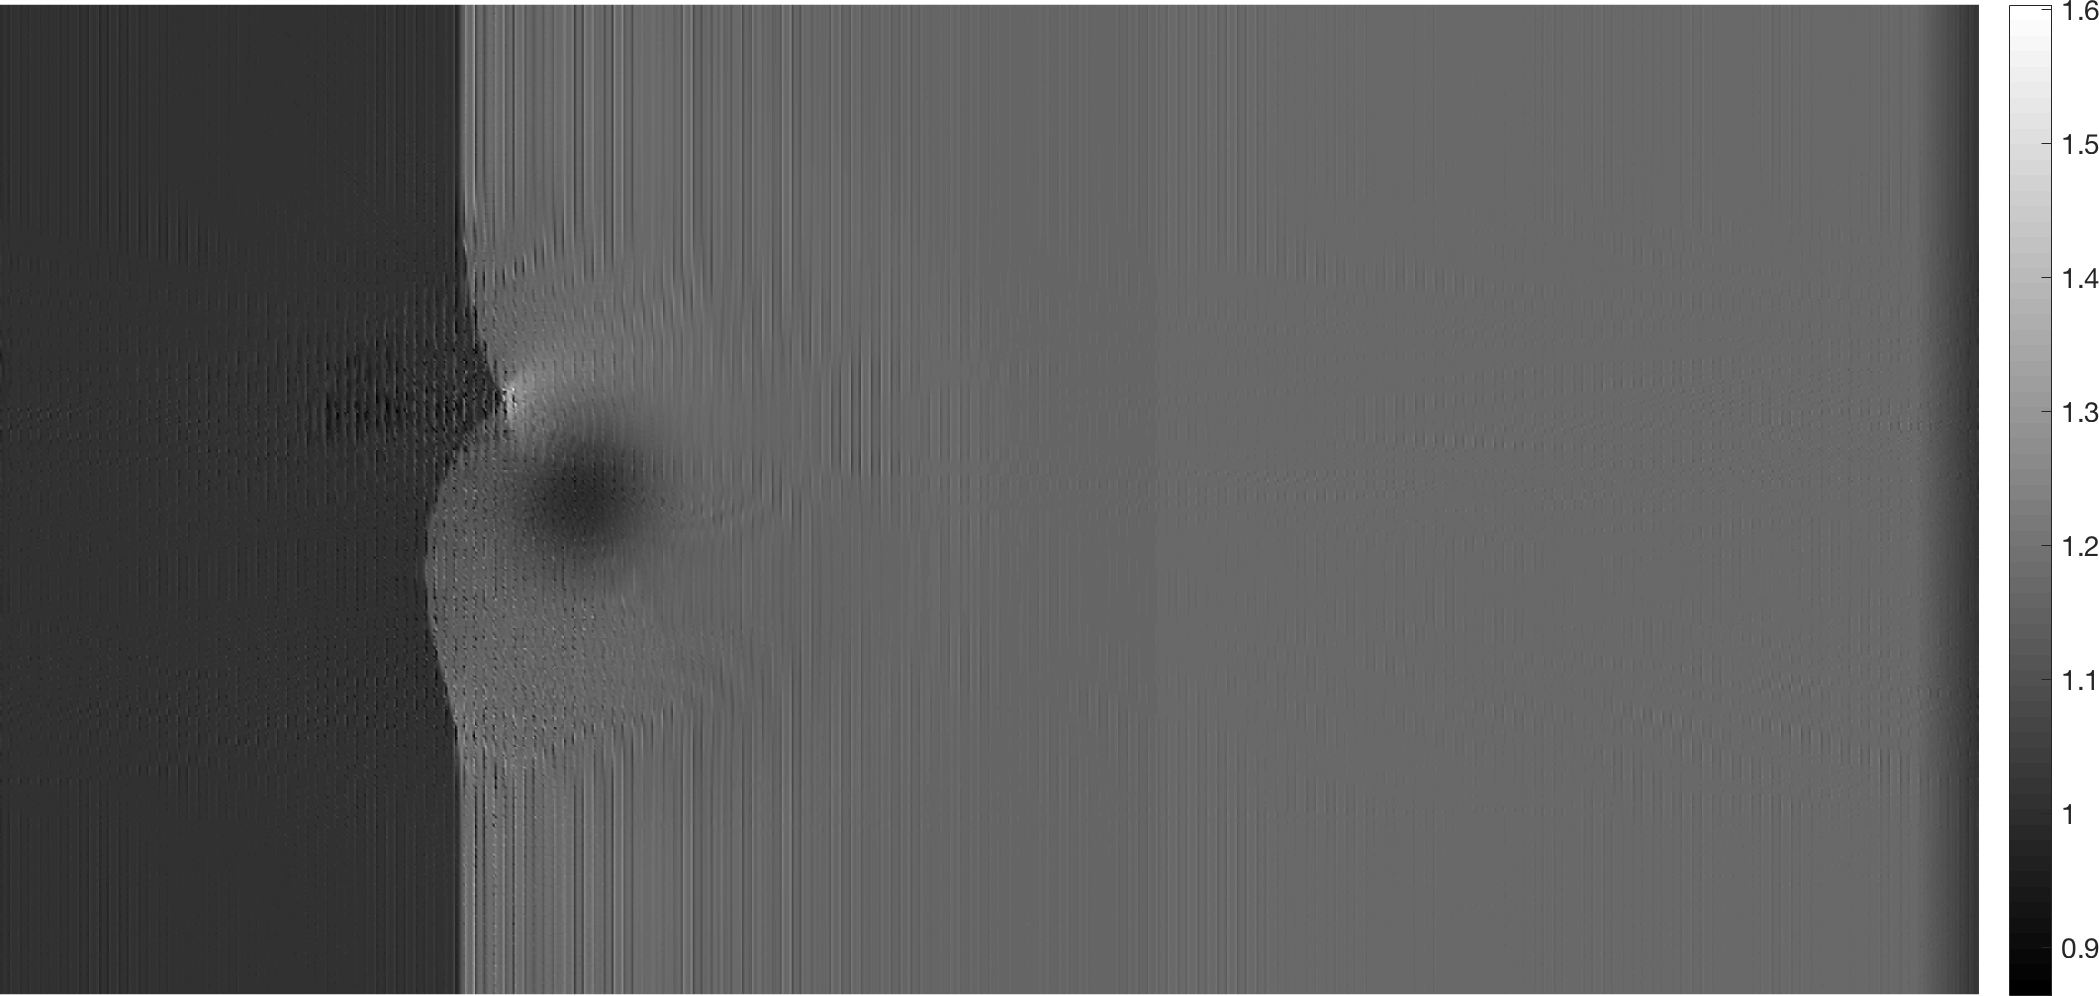
\includegraphics[width=.49\textwidth]{figs/shockVortexTp3_EC.png}}
\hspace{.05em}
\subfloat[Entropy conservative flux, $T = .7$]{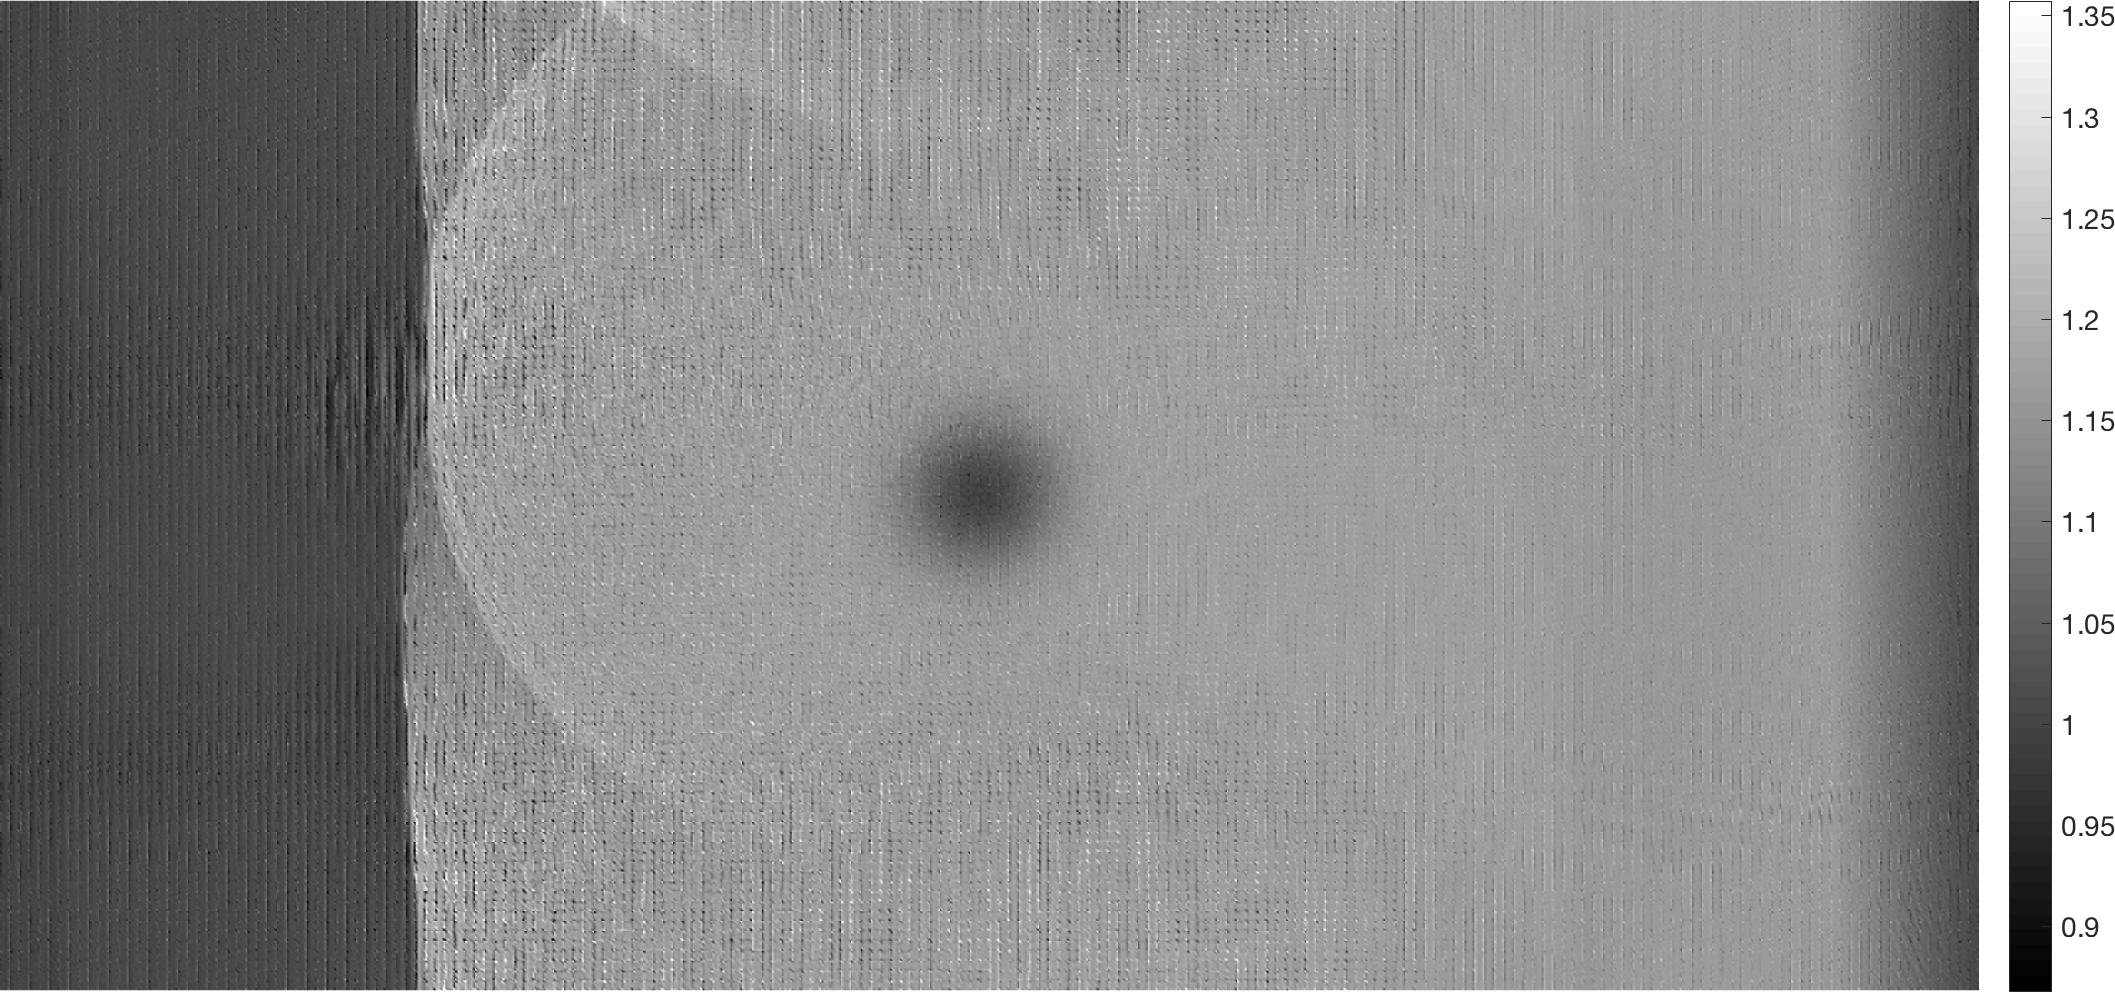
\includegraphics[width=.49\textwidth]{figs/shockVortexTp7_EC.png}}
}
\only<2>{
\subfloat[Local Lax-Friedrichs flux, $T = .3$]{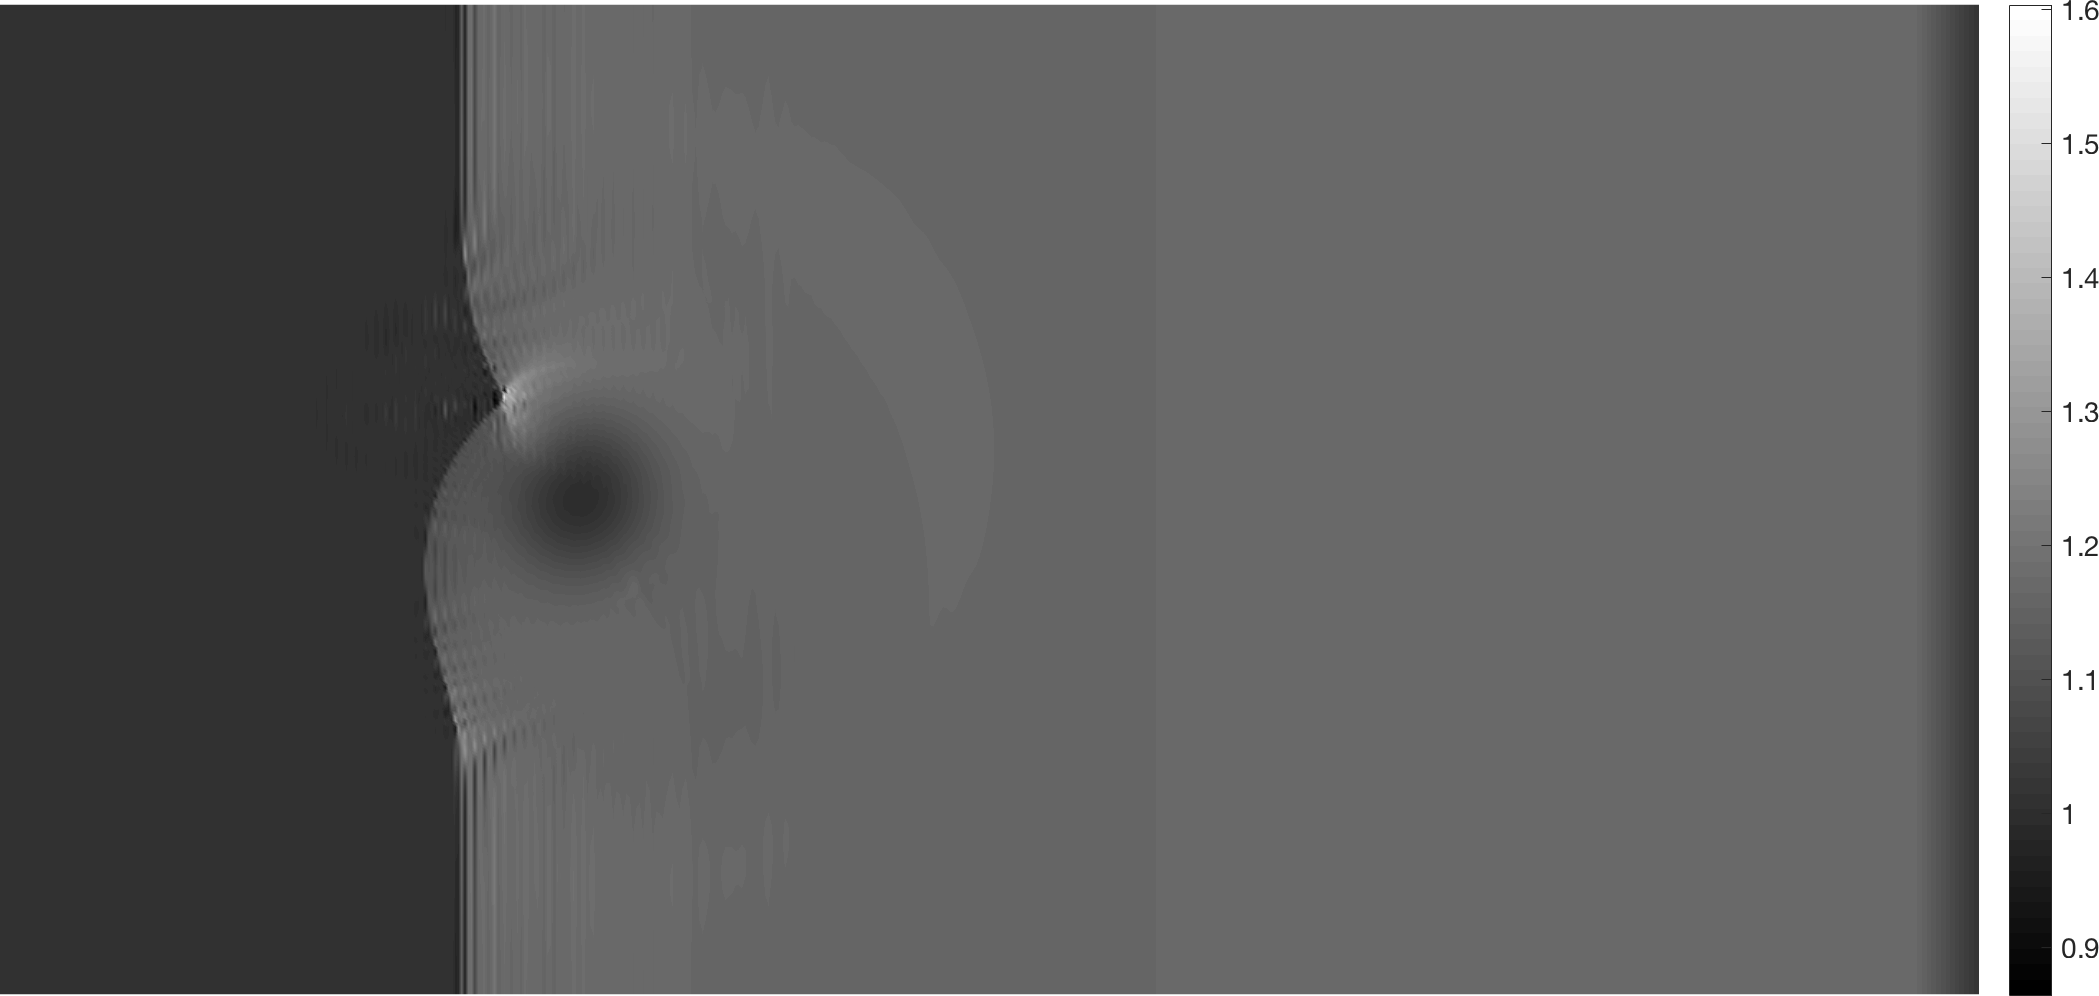
\includegraphics[width=.49\textwidth]{figs/shockVortexTp3_LF.png}}
\hspace{.05em}
\subfloat[Local Lax-Friedrichs flux, $T = .7$]{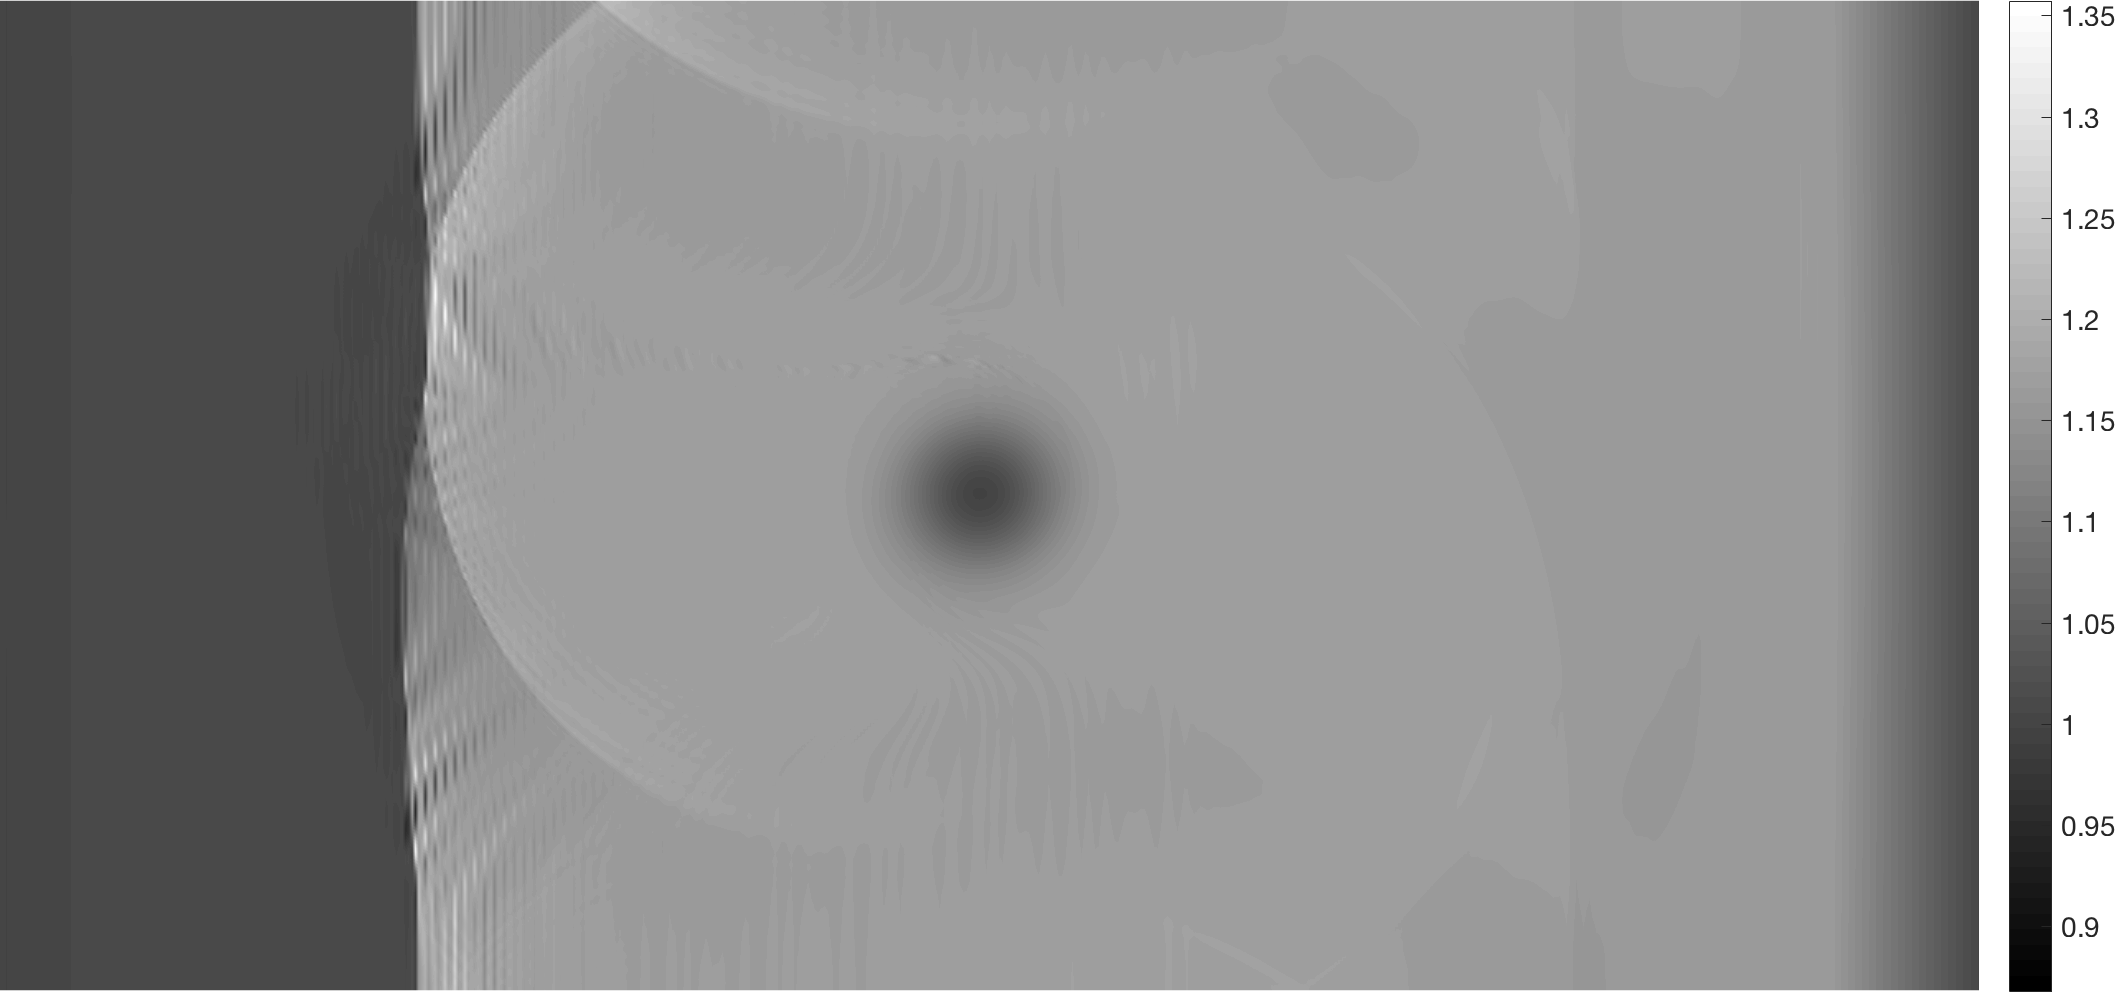
\includegraphics[width=.49\textwidth]{figs/shockVortexTp7_LF.png}}\
}
\only<3>{
\subfloat[Matrix dissipation flux, $T = .3$]{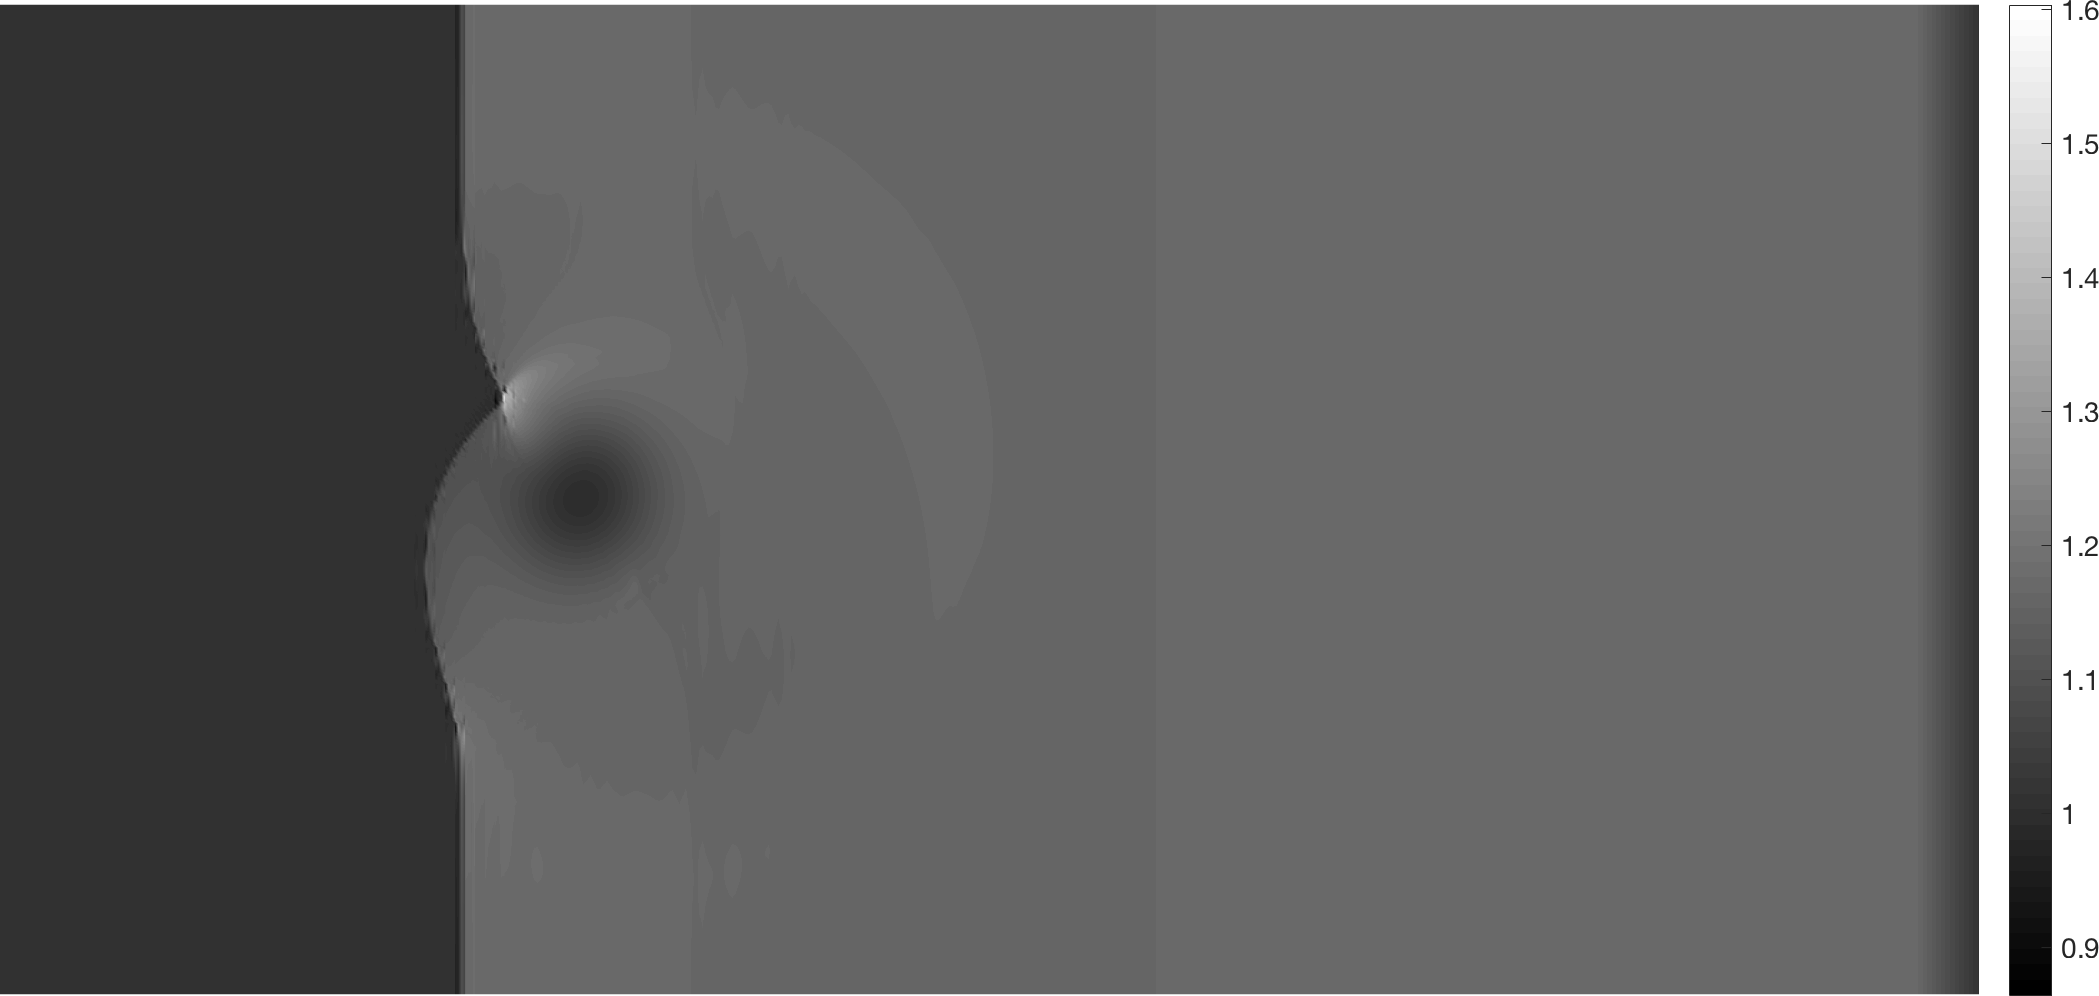
\includegraphics[width=.49\textwidth]{figs/shockVortexTp3.png}}
\hspace{.05em}
\subfloat[Matrix dissipation flux, $T = .7$]{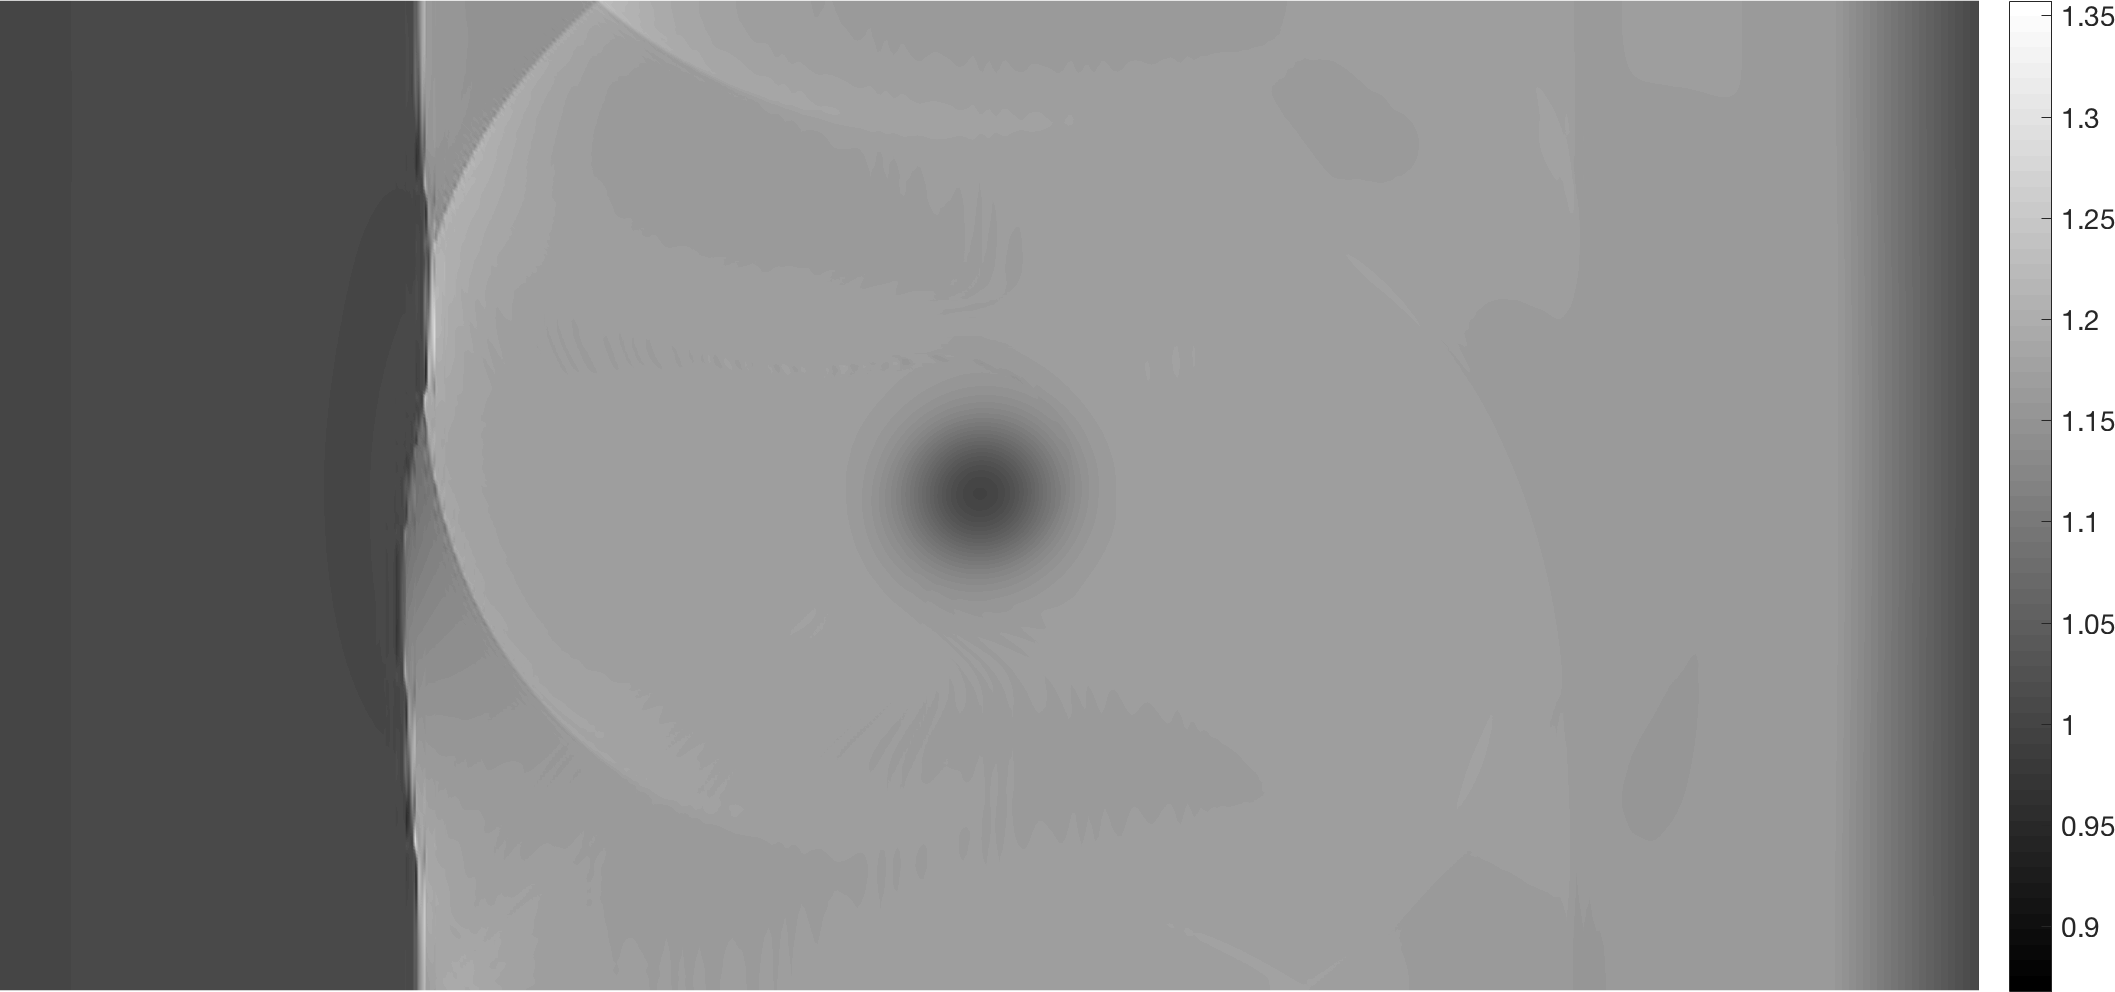
\includegraphics[width=.49\textwidth]{figs/shockVortexTp7.png}}
}
\only<4>{
\subfloat[Matrix dissipation flux, $T = .3$]{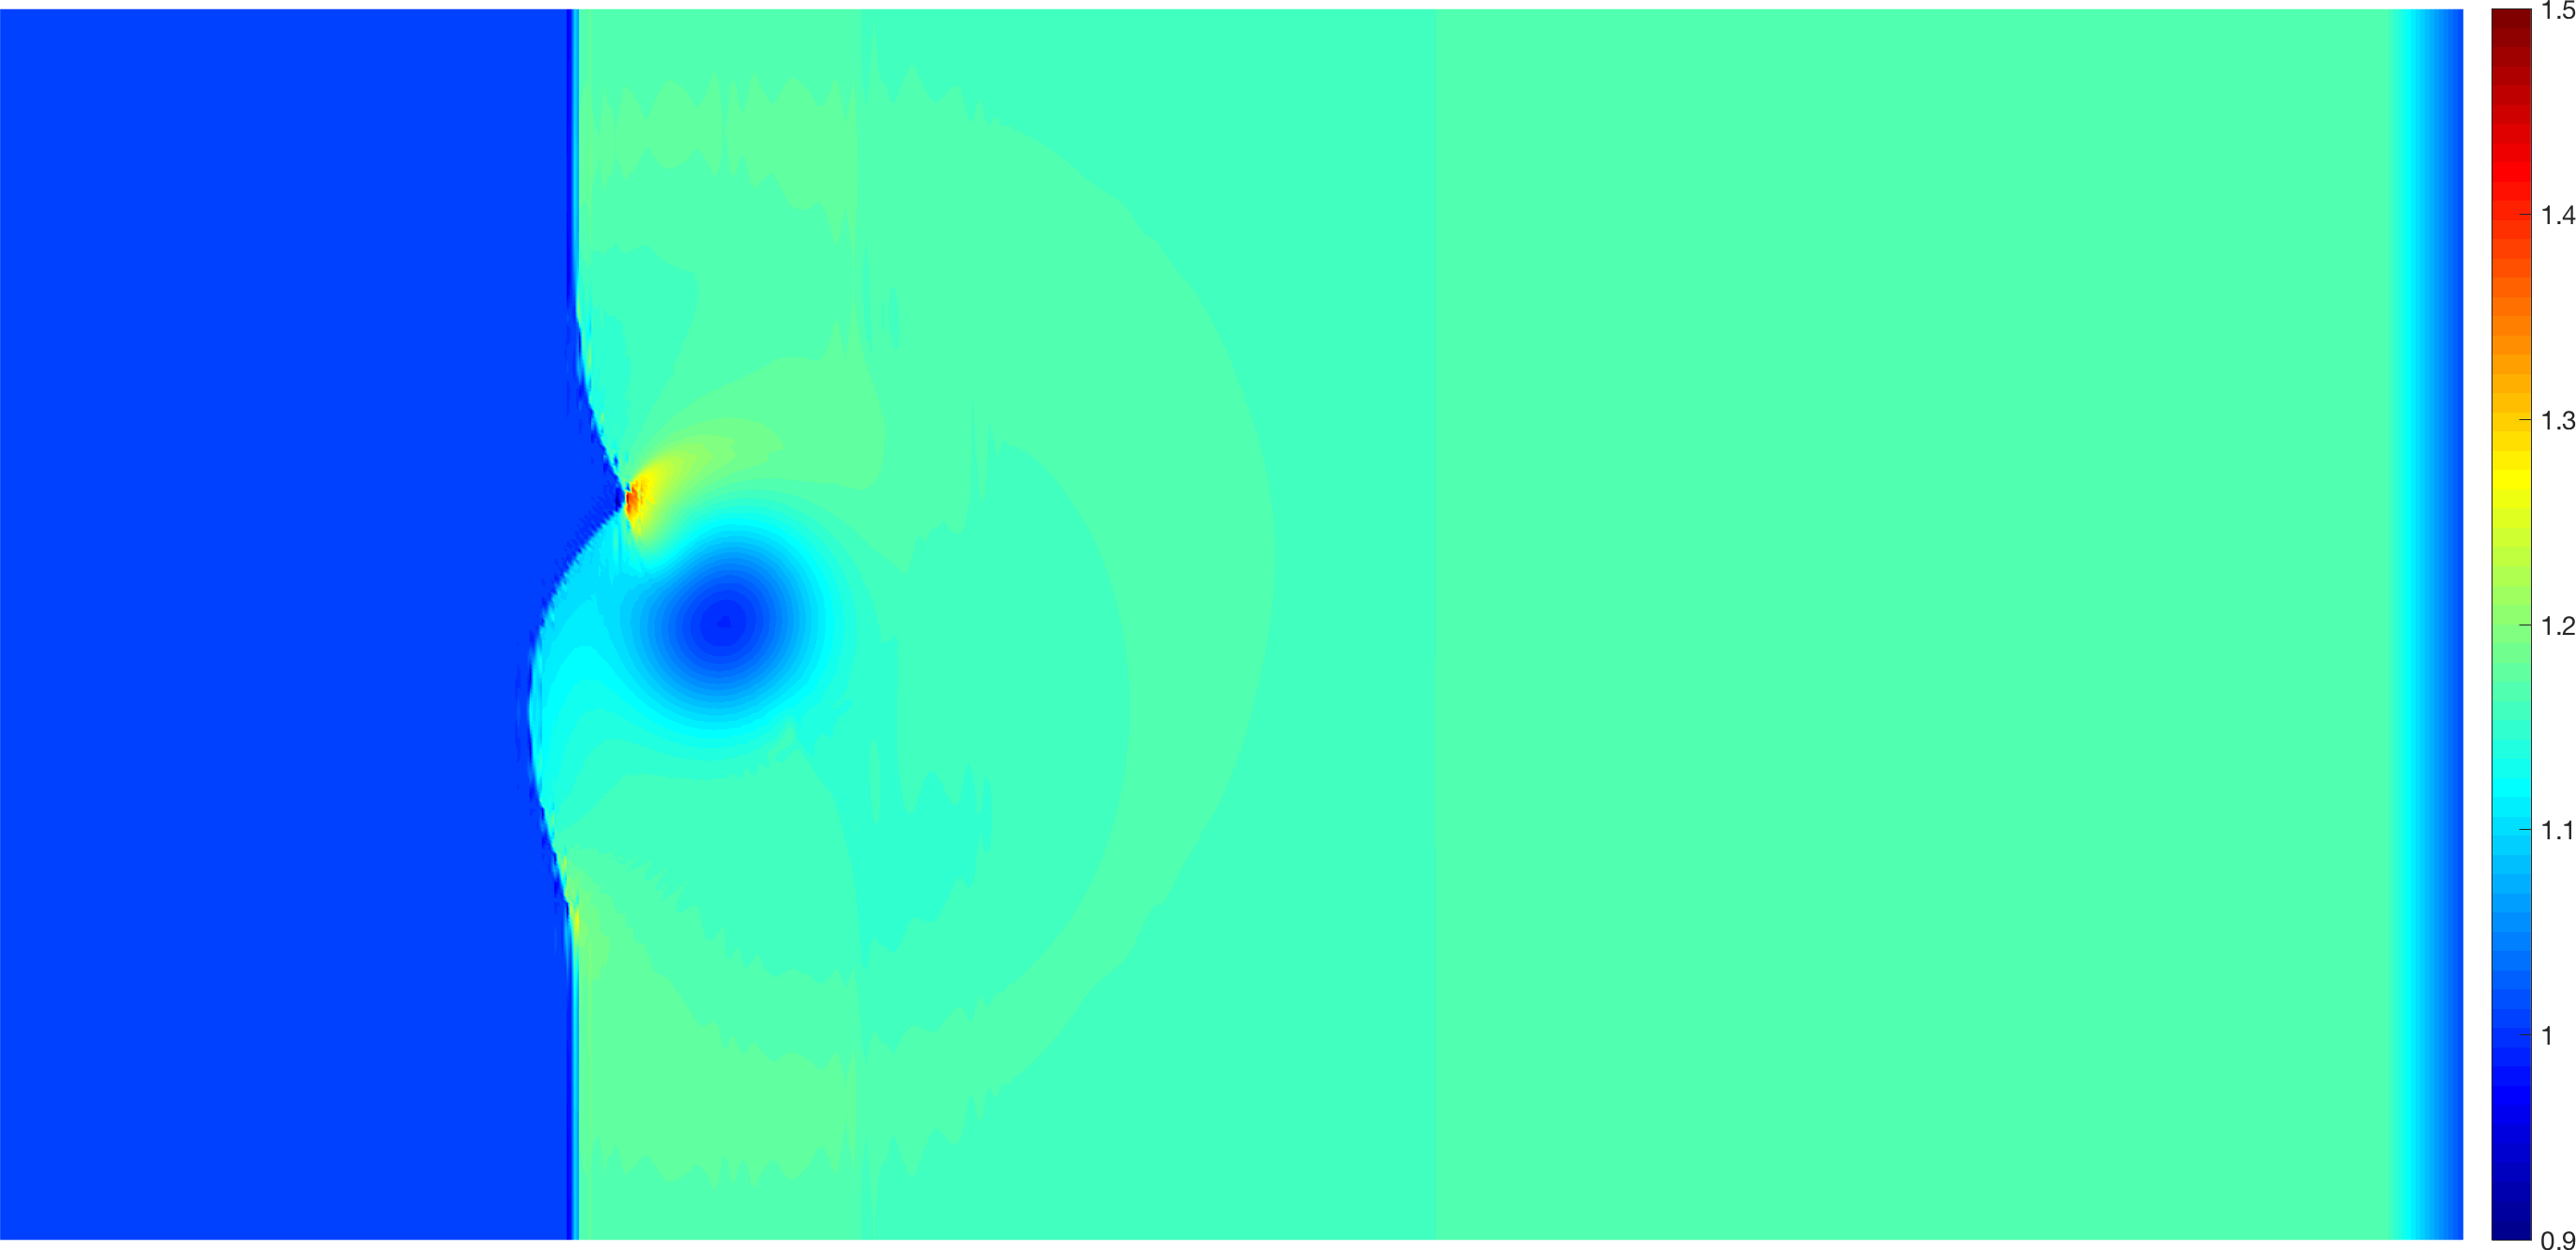
\includegraphics[width=.485\textwidth]{figs/shockVortexT3.png}}
\hspace{.05em}
\subfloat[Matrix dissipation flux, $T = .7$]{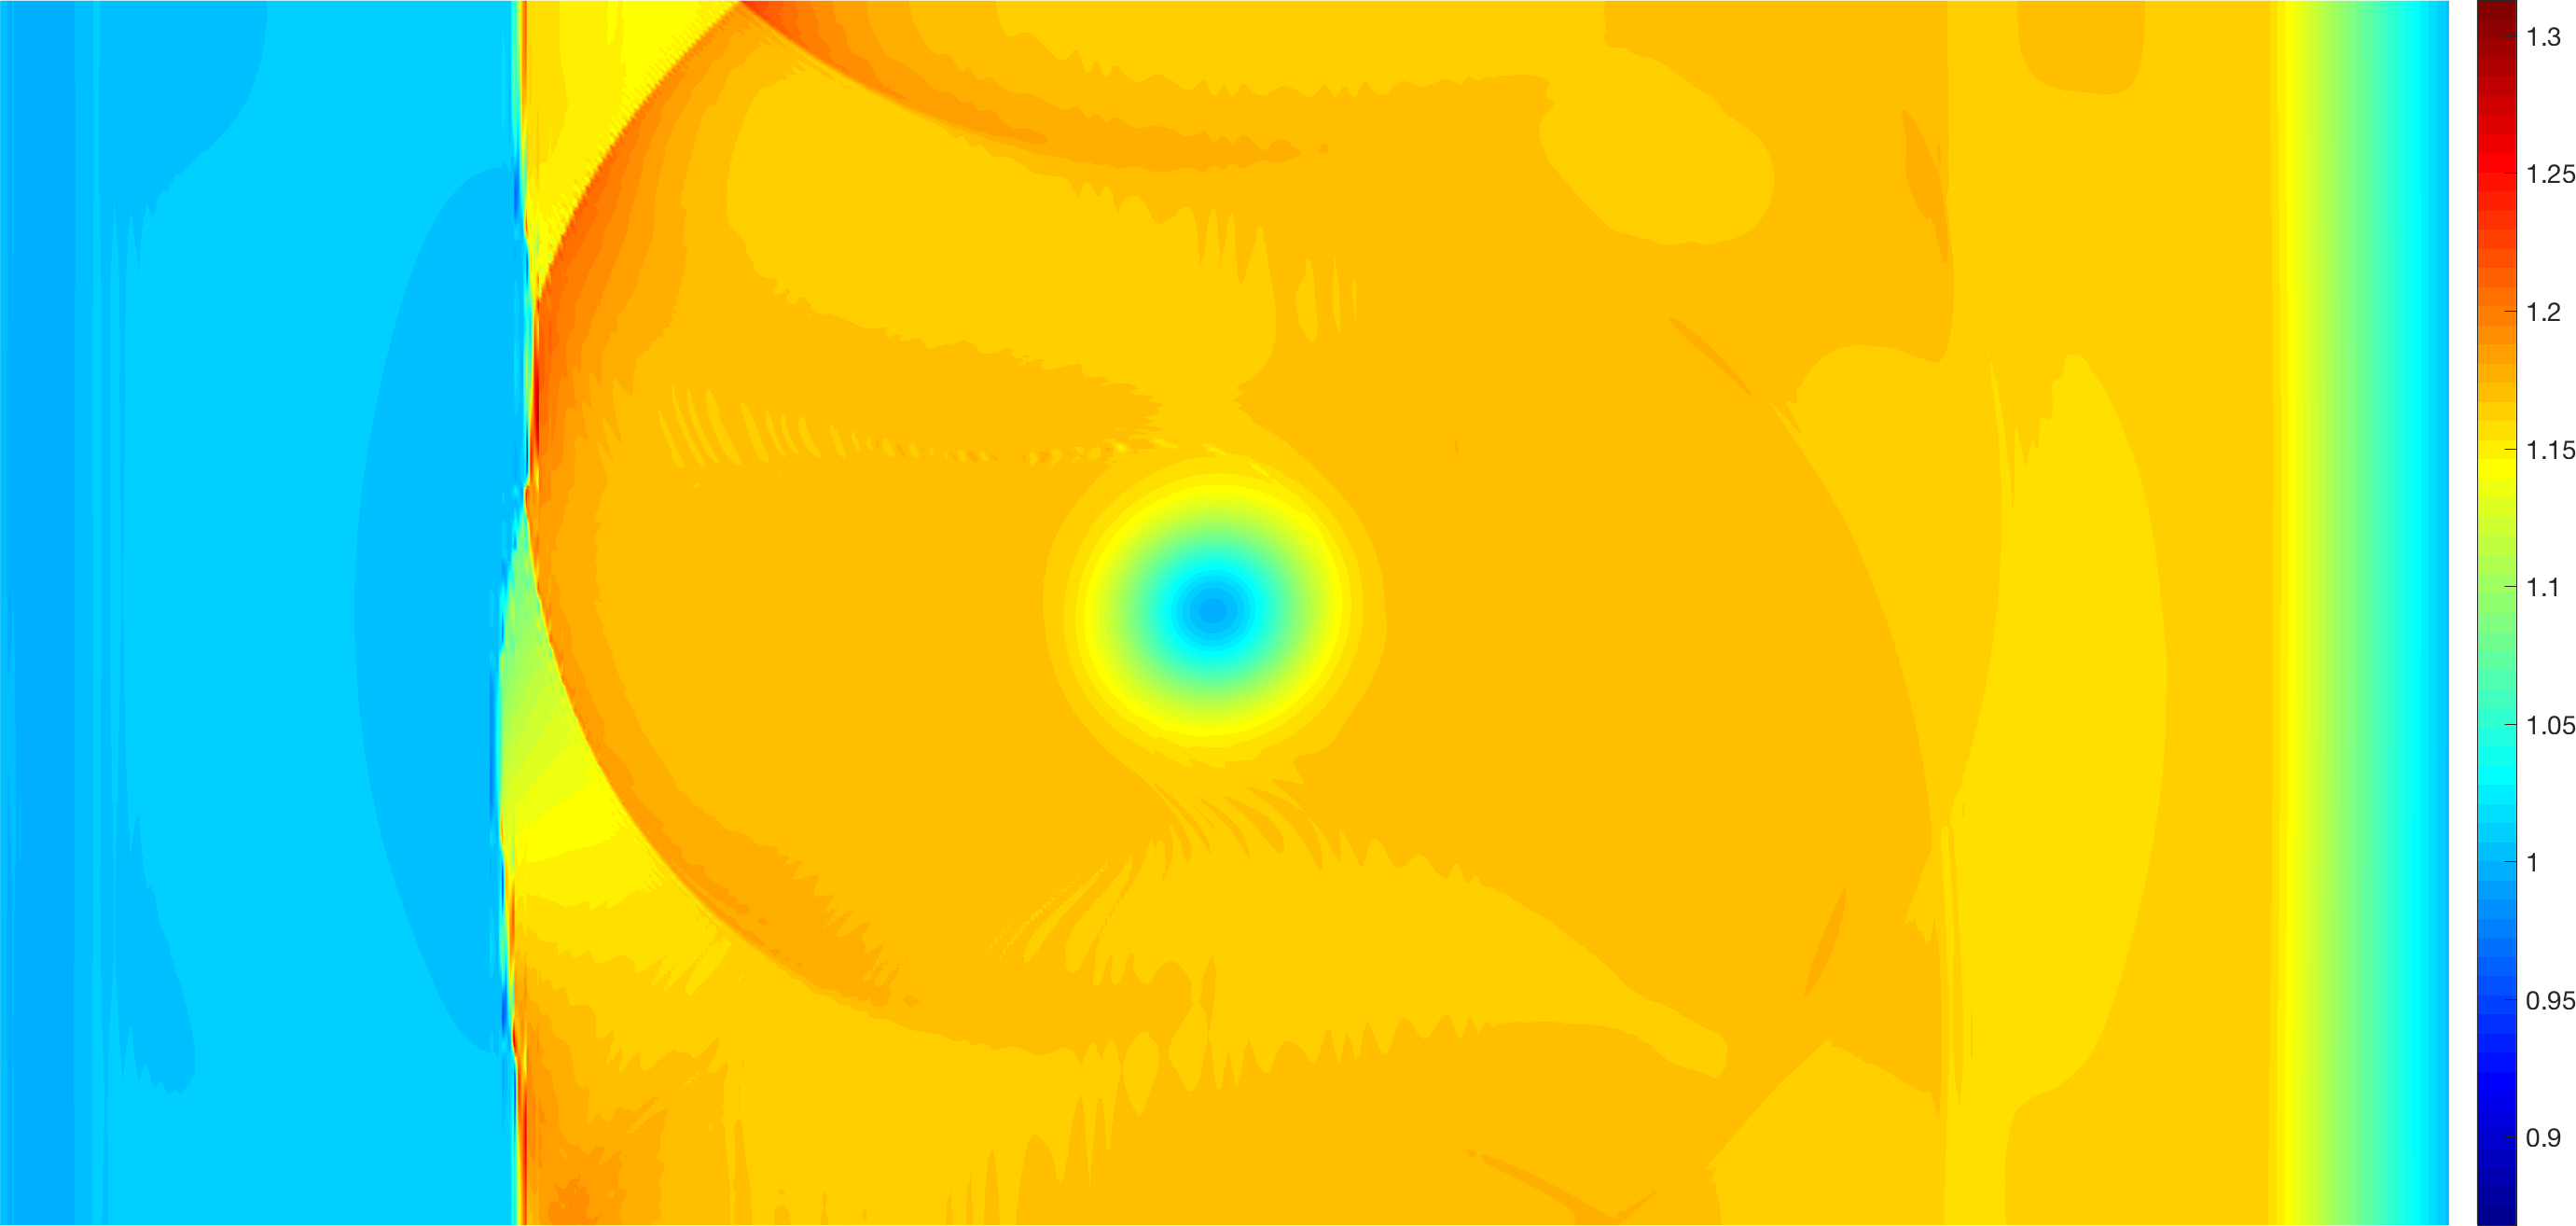
\includegraphics[width=.49\textwidth]{figs/shockVortexT7.png}}
}
\end{overlayarea}
\caption{Compressible Euler shock vortex interaction: $200\times 100$ \note{degree $N=4$} elements, $4$th order \note{explicit} RK time-stepping, no limiters or artificial viscosity.  }
\label{fig:shockvort}
\end{figure}

\let\thefootnote\relax\footnotetext{\tiny Jiang, Shu (1998).  \textit{Efficient Implementation of Weighted ENO Schemes}.}
\let\thefootnote\relax\footnotetext{\tiny Chandrashekar (2013). \textit{Kinetic energy preserving and entropy stable FV schemes for compressible Euler and NS equations.}}
\let\thefootnote\relax\footnotetext{\tiny Winters, Derigs, Gassner, and Walch (2017). \textit{A uniquely defined entropy stable matrix dissipation operator for high Mach number ideal MHD and compressible Euler simulations.}}
}

\section{Entropy stable modal DG formulations}
\frame[noframenumbering]{
\frametitle{Talk outline}
\tableofcontents[currentsection]
}


\frame{
\frametitle{Modal formulations: general bases and quadrature}
\vspace{-.5em}
\begin{figure}
\centering
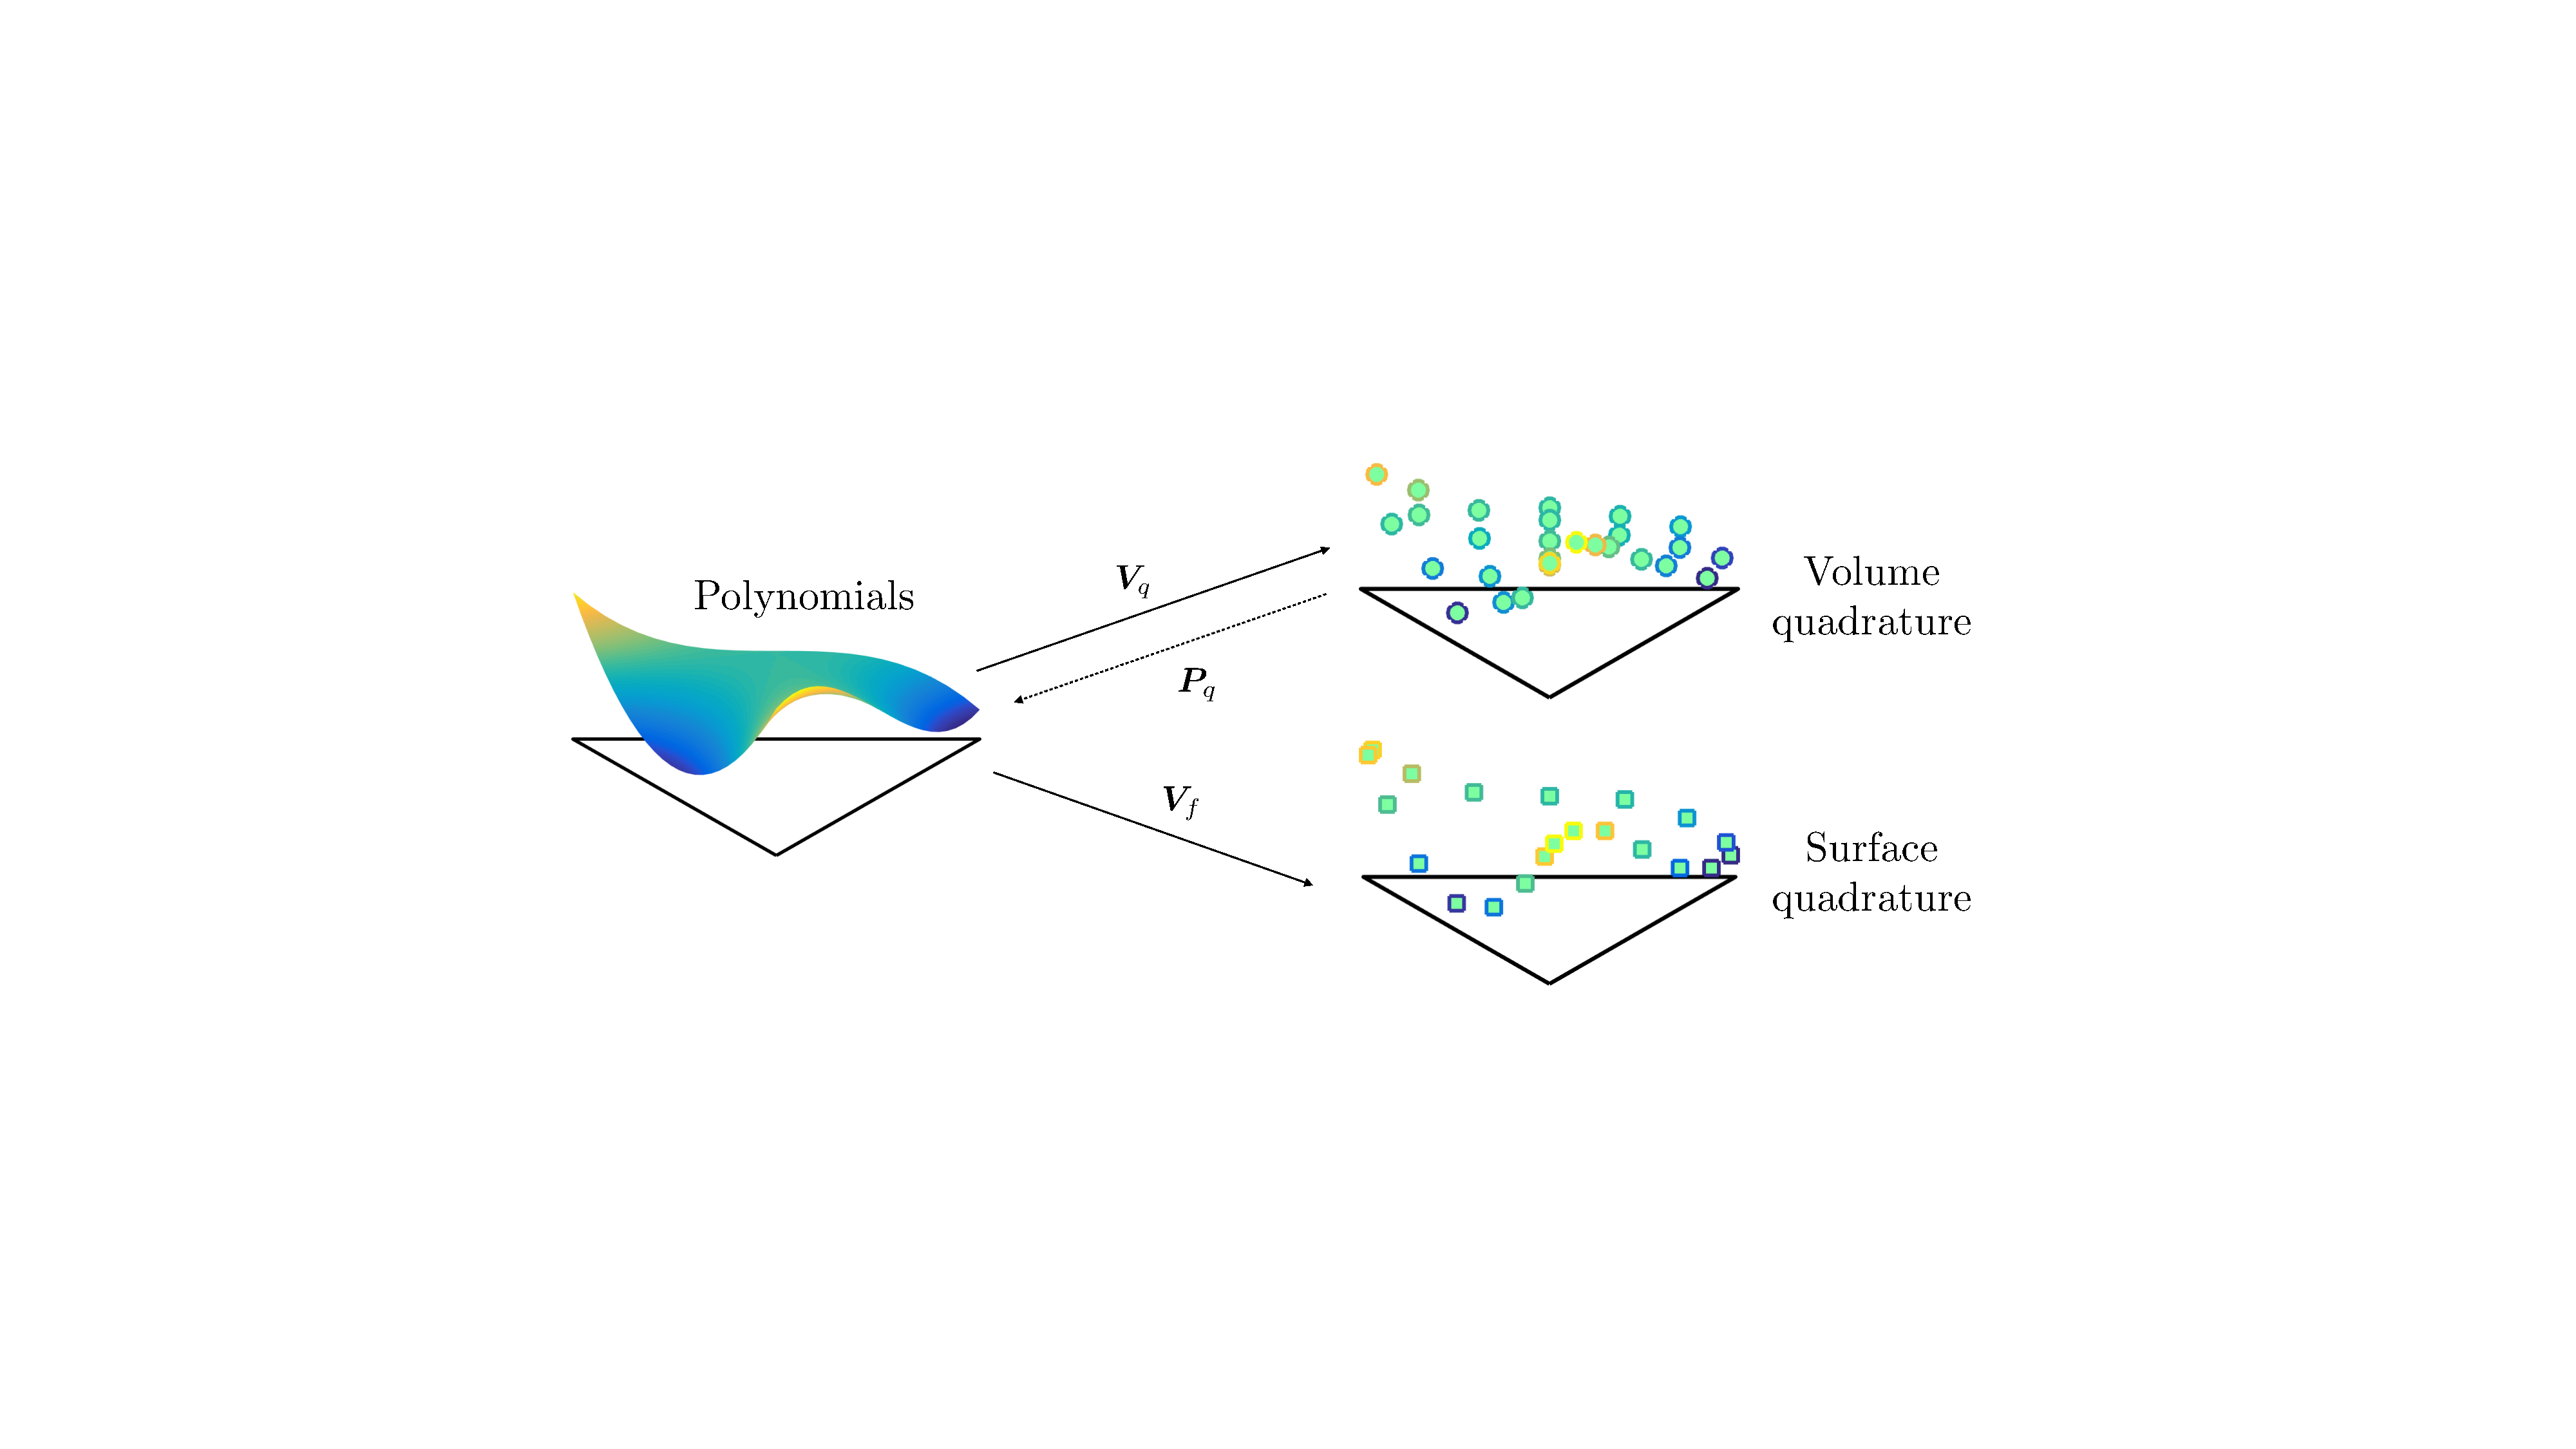
\includegraphics[width=.7\textwidth]{figs/polymap1.pdf}
\end{figure}
\vspace{-.7em}
\begin{itemize}
\item Assume degree $2N$ volume + surface quadratures $(\bm{x}^q_i,\bm{w}^q_i)$, $(\bm{x}^f_i, \bm{w}^f_i)$, and basis functions $\phi_i(\bm{x})$.  Define interpolation and weight matrices %$\bm{V}_q, \bm{V}_f, \bm{W}, \bm{W}_f$
\begin{align*}
\LRp{\bm{V}_q}_{ij} = \phi_j(\bm{x}^q_i), \qquad \LRp{\bm{V}_f}_{ij} = \phi_j(\bm{x}^f_i),\\
\bm{W} = {\rm diag}\LRp{\bm{w}^q}, \qquad \bm{W}_f = {\rm diag}\LRp{\bm{w}^f}.
\end{align*}
\item Discretize $P_N: L^2 \rightarrow P^N$, yields a quadrature-based \note{projection} matrix %$\bm{P}_q = \bm{M}^{-1}\bm{V}_q^T\bm{W}$%and \note{lifting} matrices
\[
\LRp{P_N u, v} = \LRp{u,v} \quad \forall v\in P^N \quad \Longrightarrow \quad \bm{P}_q = \bm{M}^{-1}\bm{V}_q^T\bm{W}.
\]
%\begin{gather*}
%\bm{P}_q = \bm{M}^{-1}\bm{V}_q^T\bm{W}.%, \qquad \bm{W} = {\rm diag}\LRp{\bm{w}^q}, \qquad \bm{W}_f = {\rm diag}\LRp{\bm{w}^f}.
%%\bm{P}_q = \bm{M}^{-1}\bm{V}_q^T\bm{W}, 
%%\qquad \bm{L}_f = \bm{M}^{-1}\bm{V}_f^T\bm{W}_f,\\
%%\bm{W} = {\rm diag}\LRp{\bm{w}^q}, \qquad \bm{W}_f = {\rm diag}\LRp{\bm{w}^f}.
%\end{gather*}
\end{itemize}
}


\frame{
\frametitle{Quadrature-based ``finite difference'' matrices}

\begin{figure}
\centering
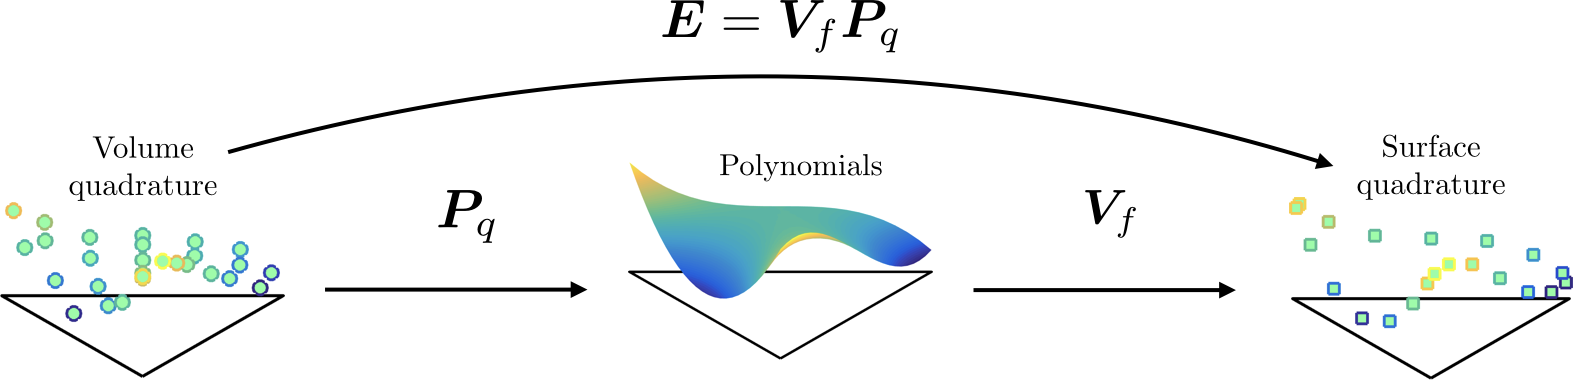
\includegraphics[width=.85\textwidth]{figs/Emap.png}
\end{figure}

\begin{itemize}
\item Matrix $\bm{D}^i_q$: evaluates $i$th derivative of $L^2$ projection $P_N$ at $\bm{x}^q$.
\[
\bm{D}^i_q = \bm{V}_q\bm{D}^i\bm{P}_q, \qquad \bm{D}^i \quad \text{exactly differentiates polynomials.}
\]
\item Generalized summation-by-parts: let $\bm{Q}_i = \bm{W}\bm{D}^i_q$ and $\bm{E} = \bm{V}_f\bm{P}_q$
\begin{gather*}
\bm{Q}_i + {\bm{Q}_i}^T = \bm{E}^T{\bm{B}_i} \bm{E}, %\LRp{\bm{V}_f\bm{P}_q}^T{\bm{B}_i}\bm{V}_f\bm{P}_q, 
 \qquad \bm{B}_i = \bm{W}_f{\rm diag}\LRp{\bm{n}_i}\\[.5em]
\Longrightarrow \boxed{\int_{\hat{D}} \pd{P_N u}{x_i}v + \int_{\hat{D}} u\pd{P_N v}{x_i} = \int_{\partial \hat{D}} \note{\LRp{P_N u}\LRp{P_N v}} \hat{n}_i.}
\end{gather*}
\end{itemize}
%\vspace{-.75em}
%\vspace{-.5em}
}

\frame{
\frametitle{Problems with generalized SBP on multiple elements}
\vspace{-1em}
\begin{figure}
\centering
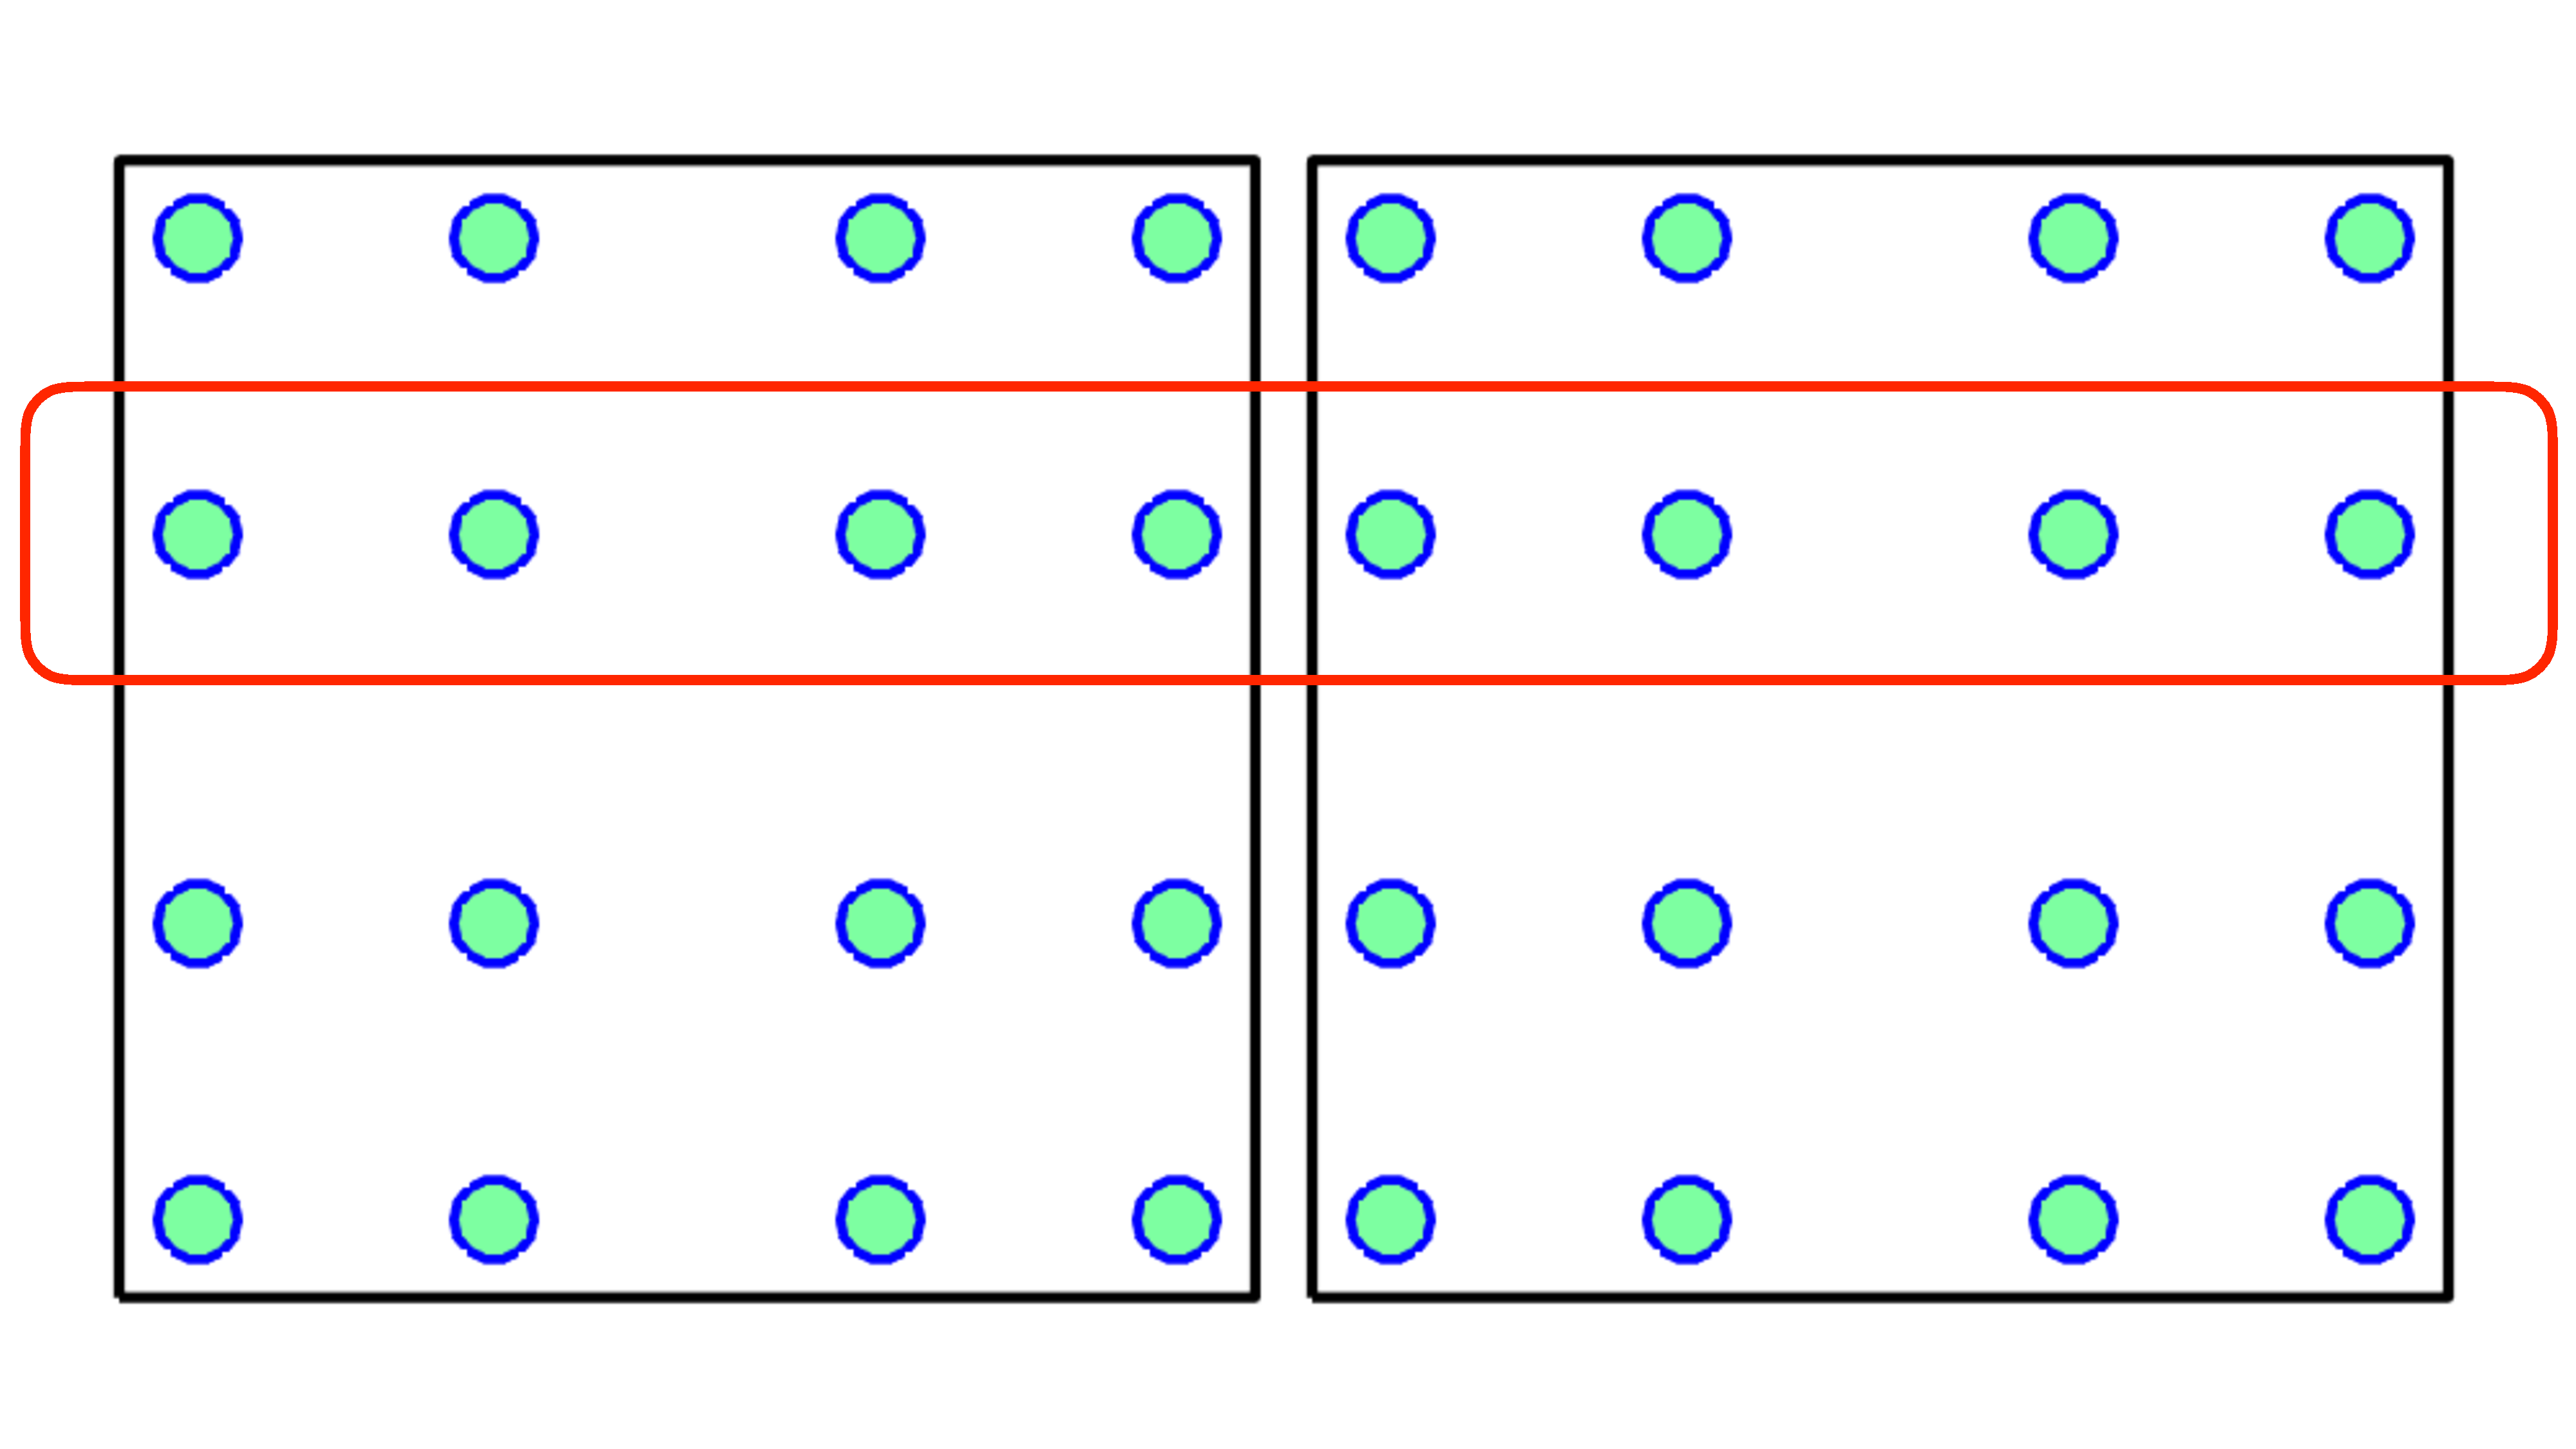
\includegraphics[width=.5\textwidth]{figs/gsbp_coupling.pdf}
\caption*{\footnotesize Coupling between quadrature nodes on neighboring elements.}
\end{figure}
\vspace{-.5em}
\begin{itemize}
\item Re-deriving the local DG formulation with GSBP operators:
\[
\only<1>{\bm{M}\td{\bm{u}}{t} + 2\LRp{\bm{Q}\circ\bm{F}_S}\bm{1} = 0.}
\only<2->{\bm{M}\td{\bm{u}}{t} + \LRp{\LRp{\bm{Q}-\bm{Q}^T}\circ\bm{F}_S}\bm{1} + \note{\LRp{\LRp{\bm{E}^T\bm{B}\bm{E}}\circ\bm{F}_S}\bm{1}} = 0.}
\]
\item<3> The presence of the interpolation matrix $\bm{E}$ increases inter-element coupling, complicates imposition of BCs.
\end{itemize}
}


\frame{
\frametitle{A ``decoupled'' SBP operator}
\begin{itemize}
%\vspace{.5em}
\item Goal: SBP property without $\bm{E}$ in the boundary terms
\begin{align*}
\bm{Q}_N  &= \LRs{
\begin{array}{cc}
\bm{Q} - \frac{1}{2}\bm{E}^T\bm{B}\bm{E} &  \frac{1}{2}\bm{E}^T\bm{B}\\
-\frac{1}{2}\bm{B}\bm{E} & \frac{1}{2}\bm{B}
\end{array}}, 
\qquad 
\label{eq:DN}
\end{align*}
\item If $\bm{Q} + \bm{Q}^T = \bm{E}^T\bm{B}\bm{E}$, then the block matrix $\bm{Q}_N$ satisfies 
\begin{gather*}
\boxed{\bm{Q}_N + {\bm{Q}_N}^T = \begin{bmatrix}
\bm{0} &\\
& \bm{B}\end{bmatrix}} \sim \boxed{\int_{-1}^1 \pd{P_Nu}{x} v + u\pd{P_Nv}{x} = \LRu{uv}_{-1}^1.}
\end{gather*}
%\[
%\]
\item $\bm{Q}_N$ approximates $f\pd{g}{x}$ by $\bm{u}$ using data at $\bm{x} = [\bm{x}_{\rm vol}, \bm{x}_{\rm face}]$ 
\[
%f\pd{g}{x} \approx 
%\LRs{\begin{array}{cc}\bm{P}_q & \bm{L}_f\end{array}} {\rm diag}\LRp{\bm{f}}\bm{D}_N \bm{g}, \qquad \bm{f}_i, \bm{g}_i = f(\bm{x}_i), g(\bm{x}_i).
\bm{M}\bm{u} = \LRs{\begin{array}{c} \bm{V}_q \\ \bm{V}_f \end{array}}^T {\rm diag}\LRp{\bm{f}}\bm{Q}_N \bm{g}, \qquad \bm{f}_i, \bm{g}_i = f(\bm{x}_i), g(\bm{x}_i).
\]
\item Reduces to traditional SBP operator under appropriate quadrature. 
\end{itemize}
}


\frame{
\frametitle{Entropy stable schemes using decoupled SBP operators}

\begin{itemize}
\item Replace SBP operator with decoupled SBP operator
\begin{overlayarea}{\textwidth}{.18\textheight}
\[
\only<1>{\bm{M}\td{\bm{u}}{t} + \note{\LRp{\LRp{\bm{Q}-\bm{Q}^T}\circ\bm{F}_S}\bm{1}} + \bm{B}\bm{f}^* = 0.}%, \qquad \text{(standard SBP)}}
\only<2>{\bm{M}\td{\bm{u}}{t} + \note{\begin{bmatrix}\bm{V}_q \\ \bm{V}_f\end{bmatrix}^T \LRp{\LRp{\bm{Q}_N-\bm{Q}_N^T}\circ\bm{F}_S}\bm{1}} + \bm{B}\bm{f}^* = 0. \qquad}
\]
\end{overlayarea}
\item $\bm{F}_S$ is the matrix of flux evaluations between solution values at \textit{both} volume and face nodes using \note{entropy projection}:
\[
\LRp{\bm{F}_S}_{ij} = \bm{f}_S\LRp{\tilde{\bm{u}}_i,\tilde{\bm{u}}_j}, \qquad \tilde{\bm{u}} = \text{ evaluate } \bm{u}\LRp{P_N\bm{v}(\bm{u})}.
\]
\item Semi-discrete scheme is verifiably entropy conservative for inexact quadrature!  Add appropriate interface dissipation (e.g.\ Lax-Friedrichs, HLLC) for entropy stability.
\end{itemize}

\let\thefootnote\relax\footnotetext{\tiny Chan (2018). \textit{On discretely entropy conservative and entropy stable discontinuous Galerkin methods.}}
\let\thefootnote\relax\footnotetext{\tiny Parsani et al.\ (2016), \textit{Entropy Stable Staggered Grid Discontinuous Spectral Collocation Methods}}
}


%\frame{
%\frametitle{Entropy conservative finite volume fluxes}
%
%\begin{itemize}
%\item<1-> Tadmor's entropy conservative numerical flux: 
%\begin{align*}
%\bm{f}_S(\bm{u},\bm{u}) &= \bm{f}(\bm{u}), \qquad \text{(consistency)} \\
%\bm{f}_S(\bm{u},\bm{v}) &= \bm{f}_S(\bm{v},\bm{u}),\qquad \text{(symmetry)} \\
%\LRp{\bm{v}_L - \bm{v}_R}^T \bm{f}\LRp{\bm{u}_L,\bm{u}_R} &= \psi_L - \psi_R, \qquad \text{(conservation)}.
%\end{align*}
%\item<2-> Example: entropy conservative flux for Burgers' equation 
%\[
%f_S(u_L,u_R) = \frac{1}{6}\LRp{u_L^2 + u_Lu_R + u_R^2}.
%\]
%\item<3-> Flux differencing: use finite volume fluxes to evaluate derivatives.% in DG methods.
%%\item<3-> Flux differencing for Burgers' equation: let $u_L = u(x), u_R = u(y)$
%%\begin{align*}
%%&f_S(u(x),u(y)) = \frac{1}{6}\LRp{u(x)^2 + u(x)u(y) + u(y)^2},\\
%%&\pd{{f}({u})}{x} \Longrightarrow \note{\LRu{2\pd{f_S\LRp{u(x),u(y)}}{x}}_{y=x}} = \frac{1}{3}\pd{u^2}{x} + \frac{1}{3}u\pd{u}{x} + \frac{1}{3}u^2\cancel{\pd{1}{x}}.
%%\end{align*}
%\end{itemize}
%
%\let\thefootnote\relax\footnotetext{\tiny Tadmor, Eitan (1987). \textit{The numerical viscosity of entropy stable schemes for systems of conservation laws. I.}}
%}


%\frame{
%\frametitle{Flux differencing: beyond split formulations}
%\begin{itemize}
%\item Fluxes do not necessarily correspond to split formulations!  
%\vspace{.5em}
%\item Example: entropy conservative flux for 1D compressible Euler
%\begin{align*}
%f^1_S(\bm{u}_L,\bm{u}_R) &= \avg{\rho}^{\log} \avg{u}\\
%f^2_S(\bm{u}_L,\bm{u}_R) &= \frac{\avg{\rho}}{2\avg{\beta}} + \avg{u}f^1_S\\
%f^3_S(\bm{u}_L,\bm{u}_R) &= f^1_S\LRp{\frac{1}{2(\gamma-1)\avg{\beta}^{\log}} - \frac{1}{2}\avg{u^2}} + \avg{u}f^2_S,
%\end{align*}
%%\vspace{.5em}
%\item Rational functions: logarithmic mean and ``inverse temperature'' $\beta$
%\[
%\avg{u}^{\log} = \frac{u_L - u_R}{\log{u_L}- \log{u_R}}, \qquad \beta = \frac{\rho}{2p}.
%\]
%\end{itemize}
%
%\let\thefootnote\relax\footnotetext{\tiny Chandreshekar (2013),  \emph{Kinetic energy preserving and entropy stable FV schemes for comp.\ Euler and NS equations.}}
%}
%
%\frame{
%\frametitle{Flux differencing: implementational details}
%\begin{itemize}
%%\item Flux differencing necessary for general nonlinear conservation laws (compressible Euler), not for split forms (Burgers, shallow water).  
%\item Define ${\bm{F}_S}$ by evaluating $\bm{f}_S$ at all combinations of quadrature points
%\[
%\LRp{\bm{F}_S}_{ij} = \bm{f}_S\LRp{u(\bm{x}_i),u(\bm{x}_j)}, \qquad \bm{x} = \LRs{\bm{x}^q,\bm{x}^f}^T.
%\]
%\item Discretize variational formulation of flux differencing using quadrature and decoupled SBP operator $\bm{Q}_N$%: for $v(x) \in P^N$, % + polynomial $L^2$ projection and lifting matrices.
%\begin{align*}
%\int_{\hat{D}} &\LRu{2\pd{f_S\LRp{u(x),u(y)}}{x}}_{y=x} v(x), \qquad \forall v \in P^N \\
%&\qquad \Longrightarrow 
%%\LRs{\begin{array}{cc} \bm{P}_q & \bm{L}_f\end{array}} {\rm diag}{\LRp{2\bm{D}_N \bm{F}_S}}.
%\LRs{\begin{array}{c} \bm{V}_q \\ \bm{V}_f\end{array}}^T {\rm diag}{\LRp{2\bm{Q}_N \bm{F}_S}}.
%\end{align*}
%%\vspace{.001em}
%\item Simpler \note{Hadamard product} reformulation: evaluate $\bm{F}_S$ on-the-fly 
%\[
%%{\rm diag}{\LRp{2\bm{D}_N \bm{F}_S}} = \LRp{2\bm{D}_N \circ \bm{F}_S}\bm{1}.
%{\rm diag}{\LRp{2\bm{Q}_N \bm{F}_S}} = \LRp{2\bm{Q}_N \circ \bm{F}_S}\bm{1}.
%\]
%\end{itemize}
%
%%\let\thefootnote\relax\footnotetext{\tiny Chandrashekar (2013). \textit{Kinetic energy preserving and entropy stable FV schemes for compressible Euler and NS equations.}}
%}


%% =================================================

%% =================================================

\section{Numerical experiments}

%\subsection{1D experiments }

\subsection{Triangular and tetrahedral meshes}

\frame[noframenumbering]{
\frametitle{Talk outline}
\only<1>{
\tableofcontents[currentsection]
}
\only<2>{
\tableofcontents[currentsection,currentsubsection]
}
}

\frame{
\frametitle{Smooth isentropic vortex and curved meshes in 2D/3D}
\vspace{-.75em}
\begin{figure}
\centering
\only<1>{
%\subfloat[Affine mesh]{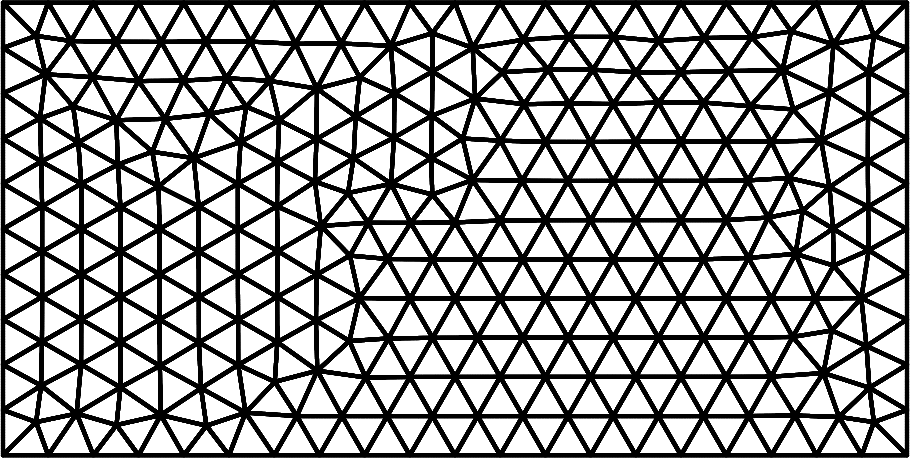
\includegraphics[width=.375\textwidth]{figs/mesh2d_affine_converge2.png}}
\subfloat[2D triangular mesh]{\raisebox{.5em}{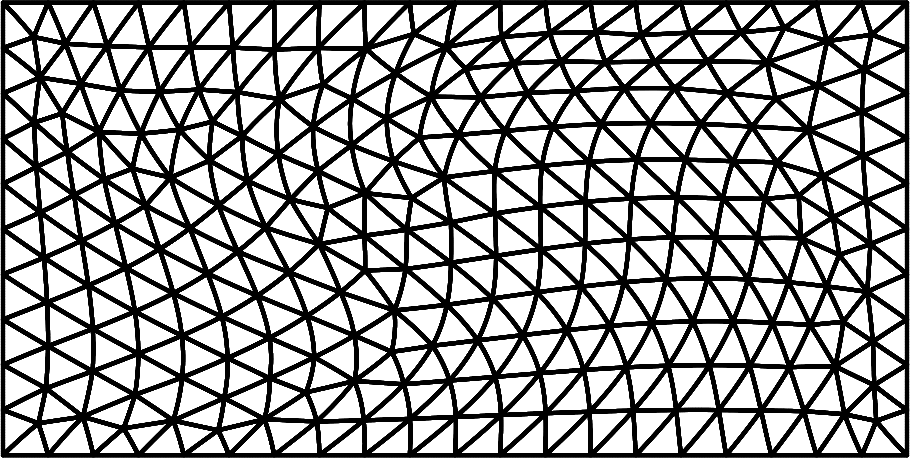
\includegraphics[width=.35\textwidth]{figs/mesh2d_curved_converge2.png}}}
\hspace{3em}
\subfloat[3D tetrahedral mesh]{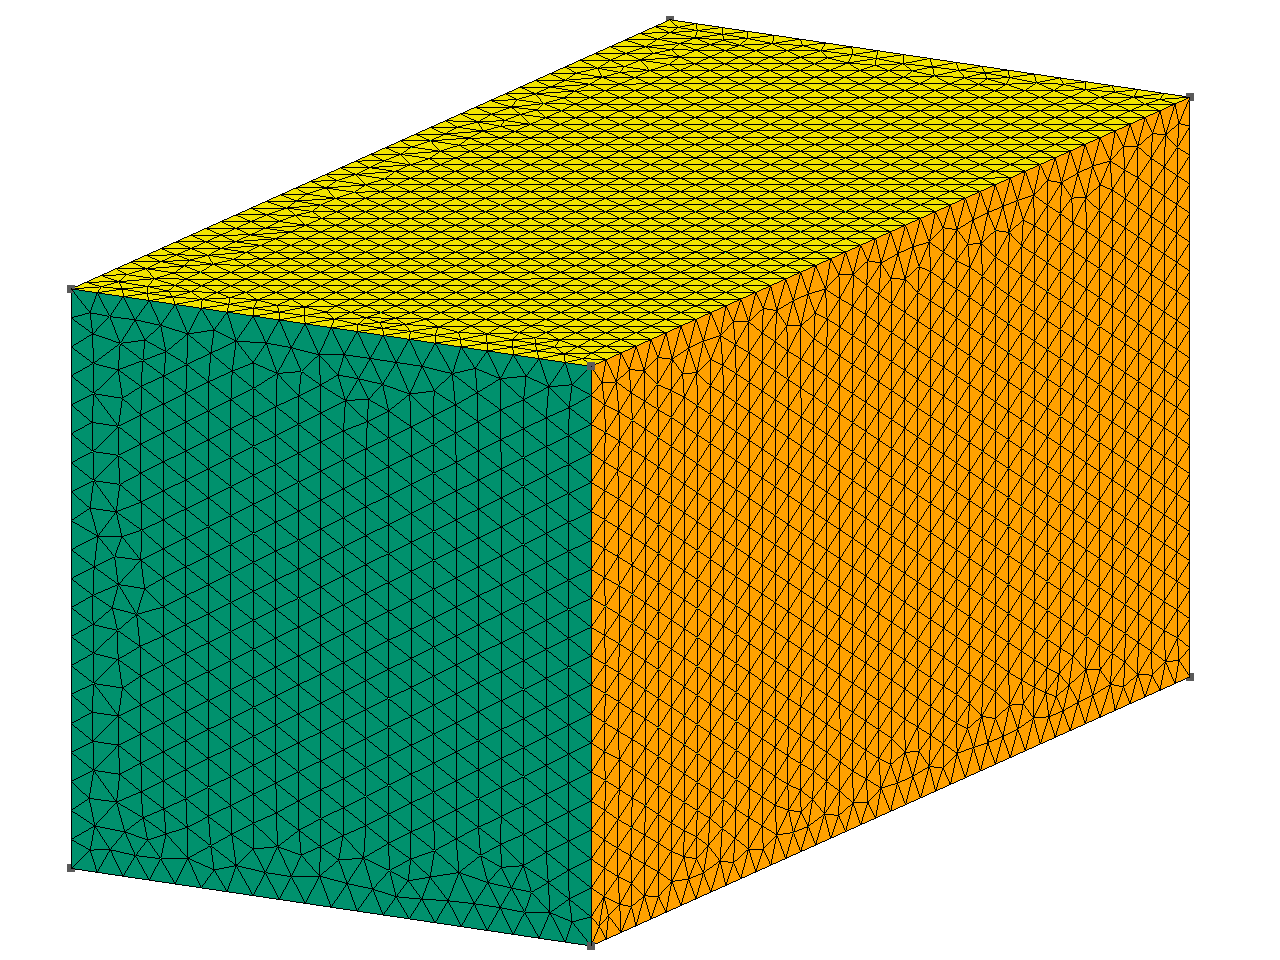
\includegraphics[width=.3\textwidth]{figs/periodicCube3.png}}
%\caption*{\footnotesize Example of 2D and 3D meshes used for convergence experiments.}% (corresponding to $h = 1$).}
}
\only<2>{
\subfloat[2D results]{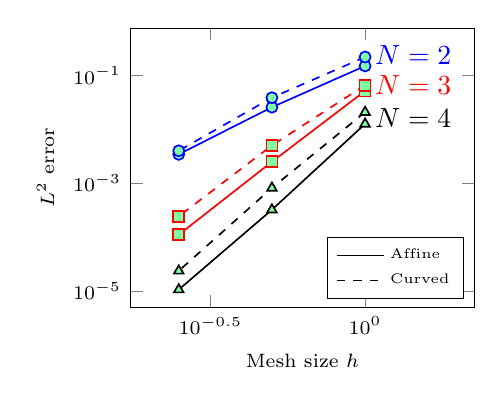
\begin{tikzpicture}
\begin{loglogaxis}[
    legend cell align=left,
    legend style={legend pos=south east, font=\tiny},
    width=.49\textwidth,    
    xlabel={Mesh size $h$},
    ylabel={$L^2$ error}, 
     ymin=5e-6, ymax=.75,    
     xmin=1.75e-1, xmax=2.25,         
    grid style=dashed,
    legend entries={Affine,Curved}
] 
\addlegendimage{no markers,black}
\addlegendimage{no markers,dashed,black}

\addplot[color=blue,mark=*,semithick, mark options={solid,fill=markercolor}]
coordinates{(1,0.149639)(0.5,0.025693)(0.25,0.00342827)} [yshift=4pt] node[right, pos=0, color=blue] {$N = 2$};
\addplot[color=blue,mark=*,dashed,semithick, mark options={solid,fill=markercolor}]
coordinates{(1,0.219501)(0.5,0.0385896)(0.25,0.0039906)};
\logLogSlopeTriangleFlip{0.285}{0.15}{0.6}{3}{blue}


\addplot[color=red,mark=square*,semithick, mark options={solid,fill=markercolor}]
coordinates{(1,0.0516053)(0.5,0.00249425)(0.25,0.000110618)}[yshift=2pt] node[right, pos=0, color=red] {$N = 3$};
\addplot[color=red,mark=square*,dashed,semithick, mark options={solid,fill=markercolor}]
coordinates{(1,0.0657418)(0.5,0.00501536)(0.25,0.000243005)};
\logLogSlopeTriangleFlip{0.285}{0.15}{0.36}{4}{red}

\addplot[color=black,mark=triangle*,semithick, mark options={solid,fill=markercolor}]
coordinates{(1,0.0125714)(0.5,0.000321559)(0.25,1.06097e-05)} [yshift=2pt] node[right, pos=0, color=black] {$N = 4$};
\addplot[color=black,mark=triangle*,dashed,semithick, mark options={solid,fill=markercolor}]
coordinates{(1,0.0207604)(0.5,0.000816006)(0.25,2.36102e-05)};
\logLogSlopeTriangle{0.31}{0.15}{0.05}{5}{black}

%\legend{$L^2$ projection,Weight-adjusted,Difference}
%\legend{Uniform, Optimal, Smoothed}
\end{loglogaxis}
\end{tikzpicture}}
\hspace{.5em}
\subfloat[3D results]{
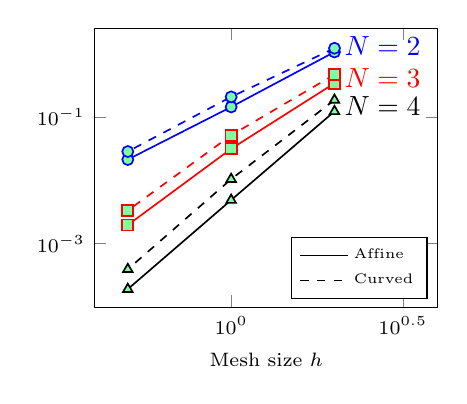
\begin{tikzpicture}
\begin{loglogaxis}[
    legend cell align=left,
    legend style={legend pos=south east, font=\tiny},
    width=.49\textwidth,    
    xlabel={Mesh size $h$},
%    ylabel={$L^2$ error}, 
     ymin=1e-4, ymax=2.5,    
     xmin=4e-1, xmax=4,         
    grid style=dashed,
    legend entries={Affine,Curved}
] 
\addlegendimage{no markers,black}
\addlegendimage{no markers,dashed,black}

\addplot[color=blue,mark=*,semithick, mark options={solid,fill=markercolor}]
coordinates{(2,1.05519)(1,0.143515)(0.5,0.0212682)}[yshift=2pt] node[right, pos=.0, color=blue] {$N = 2$};
\addplot[color=blue,mark=*,dashed,semithick, mark options={solid,fill=markercolor}]
coordinates{(2,1.20915)(1,0.2069)(0.5,0.0284505)};
\logLogSlopeTriangleFlip{0.25}{0.125}{0.6}{3}{blue}

\addplot[color=red,mark=square*,semithick, mark options={solid,fill=markercolor}]
coordinates{(2,0.339318)(1,0.0314342)(0.5,0.00197699)}[yshift=2pt] node[right, pos=0, color=red] {$N = 3$};
\addplot[color=red,mark=square*,dashed,semithick, mark options={solid,fill=markercolor}]
coordinates{(2,0.464613)(1,0.0513369)(0.5,0.00334595)};
\logLogSlopeTriangleFlip{0.25}{0.125}{0.39}{4}{red}

\addplot[color=black,mark=triangle*,semithick, mark options={solid,fill=markercolor}]
coordinates{(2,0.122229)(1,0.00488434)(0.5,0.000192453)}[yshift=2pt] node[right, pos=0, color=black] {$N = 4$};
\addplot[color=black,mark=triangle*,dashed,semithick, mark options={solid,fill=markercolor}]
coordinates{(2,0.184547)(1,0.0104361)(.5,0.0003960681)};
\logLogSlopeTriangle{0.25}{0.125}{0.05}{5}{black}

%\legend{$L^2$ projection,Weight-adjusted,Difference}
%\legend{Uniform, Optimal, Smoothed}
\end{loglogaxis}
\end{tikzpicture}}


\caption*{\footnotesize $L^2$ errors for 2D/3D isentropic vortex at $T=5$ on affine, curved meshes.}
}
\end{figure}
\only<1>{
\vspace{-.25em}
\begin{itemize}
\item ``Split'' form of derivatives on curved elements for entropy stability.
\[
J \pd{u}{x_i} = \sum_{j=1}^d J\pd{\hat{x}_j}{x_i} \pd{u}{\hat{x}_j} = \frac{1}{2} \sum_{j=1}^d \LRp{J\pd{\hat{x}_j}{x_i} \pd{u}{\hat{x}_j} +  \pd{}{\hat{x}_j}\LRp{J\pd{\hat{x}_j}{x_i}u}}.
\]
\item Discrete geometric conservation law (GCL) now a \note{necessary} condition.
%\item Generalized ``weight-adjusted'' mass lumping for curved meshes.
%\item Modify $\tilde{\bm{u}} = \bm{u}\LRp{\tilde{\bm{v}}}$, $\tilde{\bm{v}} = \tilde{P}_N^k\bm{v}(\bm{u}_h)$ using weight-adjusted projection $\tilde{P}^k_N$.
\end{itemize}
}

\let\thefootnote\relax\footnotetext{\tiny Visbal and Gaitonde (2002).  On the Use of Higher-Order Finite-Difference Schemes on Curvilinear and Deforming Meshes.}
%\let\thefootnote\relax\footnotetext{\tiny Kopriva (2006).  Metric identities and the discontinuous spectral element method on curvilinear meshes.}
\let\thefootnote\relax\footnotetext{\tiny Chan, Hewett, and Warburton (2016). \textit{Weight-adjusted discontinuous Galerkin methods: curvilinear meshes}.}
%\let\thefootnote\relax\footnotetext{\tiny Chan, Wilcox (2018). \textit{On discretely entropy stable weight-adjusted DG methods: curvilinear meshes}.}
}

%\frame{
%\frametitle{2D curved meshes: conservation of entropy}
%
%\begin{figure}
%\centering
%\subfloat[With weight-adjusted projection]{
%\begin{tikzpicture}
%\begin{semilogyaxis}[
%    legend cell align=left,
%    legend style={legend pos=south east, font=\tiny},
%    width=.48\textwidth,    
%    xlabel={Time $t$},
%    ylabel={Change in entropy $\Delta U(\bm{u})$}, 
%     ymin=1e-9, ymax=5e-4,    
%    grid style=dashed,
%] 
%
%\addplot[color=blue,mark=*,semithick, mark options={solid,fill=markercolor}]
%coordinates{(0.025641,0)(0.128205,1.81455e-05)(0.230769,1.84993e-05)(0.333333,1.81016e-05)(0.435897,2.38212e-05)(0.538462,3.43804e-05)(0.641026,3.75077e-05)(0.74359,3.80509e-05)(0.846154,4.02406e-05)(0.948718,4.57864e-05)(1.05128,5.21023e-05)(1.15385,5.52339e-05)(1.25641,5.93653e-05)(1.35897,6.53204e-05)(1.46154,7.10508e-05)(1.5641,7.58692e-05)(1.66667,8.21148e-05)(1.76923,8.86933e-05)(1.87179,9.52306e-05)(1.97436,0.000102832)};
%%\addplot[color=blue,dashed,semithick, mark options={solid,fill=markercolor}]
%%coordinates{(0.025641,9.95731e-16)(0.128205,4.11303e-15)(0.230769,1.09496e-14)(0.333333,1.86934e-14)(0.435897,1.8624e-14)(0.538462,4.82253e-14)(0.641026,2.80886e-14)(0.74359,3.34073e-14)(0.846154,3.41116e-14)(0.948718,1.12826e-14)(1.05128,1.02106e-14)(1.15385,7.27543e-15)(1.25641,3.21965e-15)(1.35897,2.70617e-15)(1.46154,2.28116e-15)(1.5641,1.01134e-14)(1.66667,9.05179e-15)(1.76923,8.96852e-15)(1.87179,2.69368e-14)(1.97436,1.20043e-15)};
%\addplot[color=red,mark=square*,semithick, mark options={solid,fill=markercolor}]
%coordinates{(0.0129032,0)(0.116129,9.54018e-07)(0.219355,8.64409e-07)(0.322581,7.28292e-07)(0.425806,1.00547e-06)(0.529032,1.54507e-06)(0.632258,1.58376e-06)(0.735484,1.48926e-06)(0.83871,1.52599e-06)(0.941935,1.77263e-06)(1.04516,2.04306e-06)(1.14839,2.10785e-06)(1.25161,2.25231e-06)(1.35484,2.49471e-06)(1.45806,2.7075e-06)(1.56129,2.86391e-06)(1.66452,3.11015e-06)(1.76774,3.35711e-06)(1.87097,3.6045e-06)(1.97419,3.88568e-06)};
%%\addplot[color=red,dotted,semithick, mark options={solid,fill=markercolor}]
%%coordinates{(0.0129032,1.00787e-15)(0.116129,2.48065e-16)(0.219355,8.43769e-15)(0.322581,1.07483e-14)(0.425806,6.18255e-15)(0.529032,4.95159e-14)(0.632258,1.19835e-14)(0.735484,3.68837e-14)(0.83871,2.35957e-14)(0.941935,1.19904e-14)(1.04516,1.73785e-14)(1.14839,7.88952e-15)(1.25161,2.44249e-14)(1.35484,6.38031e-15)(1.45806,1.78781e-14)(1.56129,5.72459e-16)(1.66452,4.02456e-15)(1.76774,1.7316e-14)(1.87097,2.50425e-14)(1.97419,3.55375e-14)};
%\addplot[color=black,mark=pentagon*,semithick, mark options={solid,fill=markercolor}]
%coordinates{(0.00647249,0)(0.110032,5.38994e-08)(0.213592,4.43651e-08)(0.317152,3.18878e-08)(0.420712,4.65967e-08)(0.524272,7.64772e-08)(0.627832,7.36288e-08)(0.731392,6.33475e-08)(0.834951,6.22881e-08)(0.938511,7.43794e-08)(1.04207,8.71374e-08)(1.14563,8.67872e-08)(1.24919,9.19998e-08)(1.35275,1.02781e-07)(1.45631,1.11204e-07)(1.55987,1.16121e-07)(1.66343,1.26634e-07)(1.76699,1.36562e-07)(1.87055,1.46567e-07)(1.97411,1.57581e-07)};
%%\addplot[color=black,dashdotted,semithick, mark options={solid,fill=markercolor}]
%%coordinates{(0.00647249,2.19226e-16)(0.110032,5.88071e-15)(0.213592,1.34059e-14)(0.317152,2.30337e-14)(0.420712,8.23647e-15)(0.524272,2.68709e-14)(0.627832,2.53304e-14)(0.731392,2.95527e-14)(0.834951,2.5948e-14)(0.938511,4.56579e-15)(1.04207,2.28428e-14)(1.14563,8.22259e-15)(1.24919,1.51094e-14)(1.35275,7.86871e-15)(1.45631,1.11508e-14)(1.55987,1.57721e-14)(1.66343,6.95624e-15)(1.76699,2.07681e-14)(1.87055,2.72421e-14)(1.97411,1.7028e-14)};
%
%% % N = 4, K= 8, dt = .25
% % N = 4, K= 8, dt = .125
% % N = 4, K= 8, dt = .0625
%
%%\legend{${\rm CFL} = .25$,${\rm CFL} = .125$,${\rm CFL} = .0625$ }
%%\legend{Uniform, Optimal, Smoothed}
%\end{semilogyaxis}
%\end{tikzpicture}
%}
%\subfloat[Without weight-adjusted projection]{
%\begin{tikzpicture}
%\begin{semilogyaxis}[
%    legend cell align=left,
%    legend style={legend pos=south east, font=\tiny},
%    width=.48\textwidth,
%    xlabel={Time $t$},
%%         ymin=1e-10, ymax=1e-1,    
%%     ymin=1e-7, ymax=1e1,
%     ymin=1e-9, ymax=5e-4,    
%%    ylabel={$L^2$ error}, 
%    grid style=dashed,
%] 
%
%\addplot[color=blue,mark=*,semithick, mark options={solid,fill=markercolor}]
%coordinates{(0.025641,0)(0.128205,4.45681e-05)(0.230769,6.82313e-05)(0.333333,0.000131517)(0.435897,0.000108761)(0.538462,8.51562e-05)(0.641026,2.94791e-05)(0.74359,3.62904e-05)(0.846154,2.97564e-05)(0.948718,9.87886e-05)(1.05128,0.000136806)(1.15385,7.64601e-05)(1.25641,0.000111044)(1.35897,5.72761e-05)(1.46154,4.27e-05)(1.5641,5.03819e-05)(1.66667,4.99789e-05)(1.76923,5.07438e-05)(1.87179,4.26361e-05)(1.97436,2.48694e-05)};
%%\addplot[color=blue,dashed,semithick, mark options={solid,fill=markercolor}]
%%coordinates{(0.025641,5.11743e-16)(0.128205,1.16547e-14)(0.230769,7.91034e-15)(0.333333,1.28231e-14)(0.435897,4.79131e-15)(0.538462,3.44134e-14)(0.641026,6.92502e-15)(0.74359,2.28047e-14)(0.846154,2.15314e-14)(0.948718,4.36456e-15)(1.05128,2.09416e-14)(1.15385,4.86763e-15)(1.25641,3.59088e-15)(1.35897,3.43475e-16)(1.46154,1.03632e-14)(1.5641,1.03598e-14)(1.66667,1.83881e-16)(1.76923,5.94663e-15)(1.87179,3.18252e-14)(1.97436,1.88495e-14)};
%\addplot[color=red,mark=square*,semithick, mark options={solid,fill=markercolor}]
%coordinates{(0.0129032,0)(0.116129,6.48664e-05)(0.219355,8.24474e-05)(0.322581,0.000152373)(0.425806,0.000138342)(0.529032,0.000126709)(0.632258,1.85501e-05)(0.735484,6.98555e-05)(0.83871,7.53129e-05)(0.941935,0.00013915)(1.04516,0.000196476)(1.14839,0.000133645)(1.25161,0.000173751)(1.35484,0.000126668)(1.45806,0.000116008)(1.56129,0.000127919)(1.66452,0.0001343)(1.76774,0.000140992)(1.87097,0.00013971)(1.97419,0.0001291)};
%%\addplot[color=red,dotted,semithick, mark options={solid,fill=markercolor}]
%%coordinates{(0.0129032,3.00107e-16)(0.116129,6.93196e-15)(0.219355,1.00198e-14)(0.322581,7.79932e-15)(0.425806,2.48759e-15)(0.529032,3.46181e-14)(0.632258,1.7205e-14)(0.735484,2.30718e-14)(0.83871,3.0146e-14)(0.941935,9.4369e-15)(1.04516,1.07969e-14)(1.14839,5.59275e-15)(1.25161,5.34295e-15)(1.35484,5.7801e-15)(1.45806,8.74648e-15)(1.56129,1.24137e-14)(1.66452,2.95597e-15)(1.76774,2.64441e-14)(1.87097,2.58023e-14)(1.97419,6.984e-15)};
%\addplot[color=black,mark=pentagon*,semithick, mark options={solid,fill=markercolor}]
%coordinates{(0.00647249,0)(0.110032,6.52844e-05)(0.213592,8.08628e-05)(0.317152,0.000153077)(0.420712,0.000141625)(0.524272,0.000130883)(0.627832,2.58046e-05)(0.731392,6.81127e-05)(0.834951,7.92926e-05)(0.938511,0.000137768)(1.04207,0.000201777)(1.14563,0.000136705)(1.24919,0.000177364)(1.35275,0.000131153)(1.45631,0.000119851)(1.55987,0.000131686)(1.66343,0.000138676)(1.76699,0.00014539)(1.87055,0.000144608)(1.97411,0.000134142)};
%%\addplot[color=black,dashdotted,semithick, mark options={solid,fill=markercolor}]
%%coordinates{(0.00647249,7.31403e-16)(0.110032,1.05055e-14)(0.213592,2.58127e-15)(0.317152,1.04916e-14)(0.420712,5.12437e-15)(0.524272,4.40203e-14)(0.627832,1.147e-14)(0.731392,2.81025e-14)(0.834951,3.01946e-14)(0.938511,4.51028e-15)(1.04207,1.096e-14)(1.14563,6.11317e-15)(1.24919,3.69843e-15)(1.35275,6.47399e-15)(1.45631,9.41608e-15)(1.55987,1.58901e-15)(1.66343,6.39766e-15)(1.76699,1.56819e-14)(1.87055,2.11949e-14)(1.97411,1.12063e-14)};
%
%%\legend{Geo-$(N+1)$, $h^{N+2}$, Geo-$N$, $h^{N+1}$}
%\legend{${\rm CFL} = .25$,${\rm CFL} = .125$,${\rm CFL} = .0625$ }
%\end{semilogyaxis}
%\end{tikzpicture}
%}
%%\subfloat[Convergence of $\Delta S(\bm{u})$]{
%%\begin{tikzpicture}
%%\begin{loglogaxis}[
%%    legend cell align=left,
%%    legend style={legend pos=south east, font=\tiny},
%%    width=.475\textwidth,    
%%    xlabel={Mesh size $h$},
%%    ylabel={$L^2$ error}, 
%%     ymin=5e-6, ymax=2,    
%%     xmin=1e-1, xmax=2.5,         
%%    grid style=dashed,
%%    legend entries={Affine,Curved}
%%] 
%%\addlegendimage{no markers,black}
%%\addlegendimage{no markers,dashed,black}
%%
%%\addplot[color=blue,mark=*,semithick, mark options={solid,fill=markercolor}]
%%coordinates{(2,1.06717)(1,0.149639)(0.5,0.025693)(0.25,0.00342827)} [yshift=4pt] node[left, pos=1.05, color=blue] {$N = 2$};
%%\logLogSlopeTriangleFlip{0.45}{0.15}{0.575}{3}{blue}
%%
%%
%%%\legend{$L^2$ projection,Weight-adjusted,Difference}
%%%\legend{Uniform, Optimal, Smoothed}
%%\end{loglogaxis}
%%\end{tikzpicture}
%%}
%\caption{Change in entropy under an entropy conservative flux with $N=4$.  In both cases, the spatial formulation tested with $\tilde{\bm{v}} = P_N\bm{v}(\bm{u})$ is $O\LRp{10^{-14}}$. }
%%\label{fig:dSconverge}
%\end{figure}
%}

%\frame{
%\frametitle{3D isentropic vortex} 
%\begin{figure}
%\centering
%\subfloat[Affine mesh for $h = 1/2$]{\raisebox{2em}{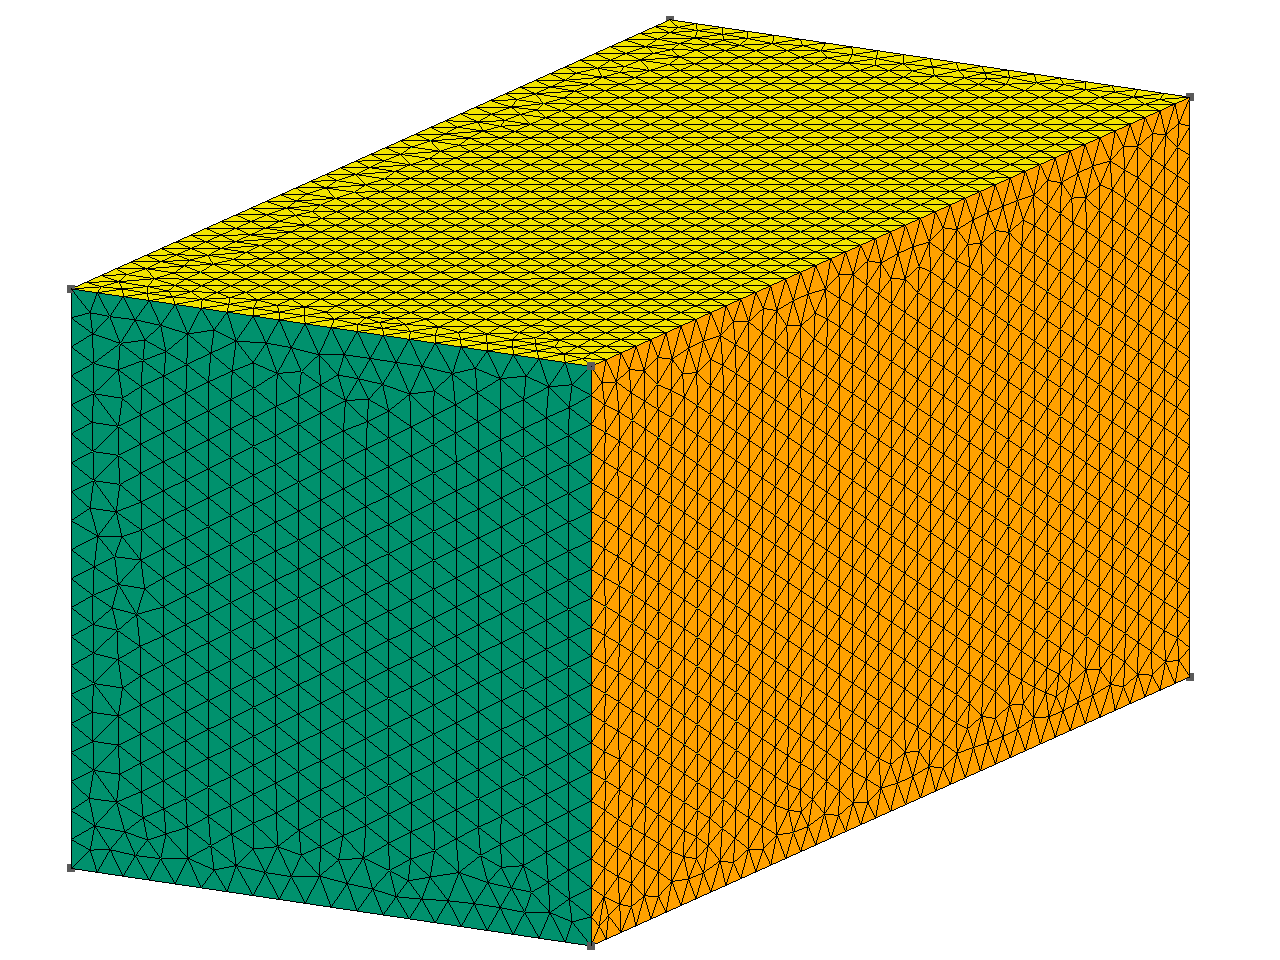
\includegraphics[width=.425\textwidth]{figs/periodicCube3.png}}\label{subfig:mesh3d}}
%\subfloat[$L^2$ errors]{\begin{tikzpicture}
%\begin{loglogaxis}[
%    legend cell align=left,
%    legend style={legend pos=south east, font=\tiny},
%    width=.55\textwidth,    
%    xlabel={Mesh size $h$},
%    ylabel={$L^2$ error}, 
%     ymin=1e-4, ymax=2,    
%     xmin=4e-1, xmax=4,         
%    grid style=dashed,
%    legend entries={Affine,Curved}
%] 
%\addlegendimage{no markers,black}
%\addlegendimage{no markers,dashed,black}
%
%\addplot[color=blue,mark=*,semithick, mark options={solid,fill=markercolor}]
%coordinates{(2,1.05519)(1,0.143515)(0.5,0.0212682)}[yshift=2pt] node[right, pos=.0, color=blue] {$N = 2$};
%\addplot[color=blue,mark=*,dashed,semithick, mark options={solid,fill=markercolor}]
%coordinates{(2,1.20915)(1,0.2069)(0.5,0.0284505)};
%\logLogSlopeTriangle{0.25}{0.125}{0.525}{3}{blue}
%
%\addplot[color=red,mark=square*,semithick, mark options={solid,fill=markercolor}]
%coordinates{(2,0.339318)(1,0.0314342)(0.5,0.00197699)}[yshift=2pt] node[right, pos=0, color=red] {$N = 3$};
%\addplot[color=red,mark=square*,dashed,semithick, mark options={solid,fill=markercolor}]
%coordinates{(2,0.464613)(1,0.0513369)(0.5,0.00334595)};
%\logLogSlopeTriangle{0.25}{0.125}{0.3}{4}{red}
%
%\addplot[color=black,mark=triangle*,semithick, mark options={solid,fill=markercolor}]
%coordinates{(2,0.122229)(1,0.00488434)(0.5,0.000192453)}[yshift=2pt] node[right, pos=0, color=black] {$N = 4$};
%\addplot[color=black,mark=triangle*,dashed,semithick, mark options={solid,fill=markercolor}]
%coordinates{(2,0.184547)(1,0.0104361)(.5,0.0003960681)};
%\logLogSlopeTriangle{0.25}{0.125}{0.05}{5}{black}
%
%%\legend{$L^2$ projection,Weight-adjusted,Difference}
%%\legend{Uniform, Optimal, Smoothed}
%\end{loglogaxis}
%\end{tikzpicture}}
%\caption{$L^2$ errors at $T=5$ for the 3D isentropic vortex on affine, curved meshes.}
%\label{fig:converge3d}
%\end{figure}
%}

\frame{
\frametitle{Inviscid Taylor-Green vortex} 
%\vspace{-1em}
\begin{figure}
\centering
\includegraphics[width=.65\textwidth]{figs/taylorgreen.png}
\caption{Isocontours of $z$-vorticity for Taylor-Green at $t = 0, 10$ seconds.}
\end{figure}
%\vspace{-.5em}
\begin{itemize}
\item Simple turbulence-like behavior (generation of small scales).
%\vspace{.25em}
\item Inviscid Taylor-Green: tests robustness w.r.t.\ under-resolved solutions.
\end{itemize}
\let\thefootnote\relax\footnotetext{\tiny \url{https://how4.cenaero.be/content/bs1-dns-taylor-green-vortex-re1600}.}
}

\frame{
\frametitle{Inviscid Taylor-Green vortex: robust w.r.t.\ under-resolution} 
%\vspace{-.5em}
\begin{figure}
%\centering
%\only<1>{
%\subfloat[Kinetic energy ]{
%\begin{tikzpicture}
%\begin{axis}[
%        scaled ticks=false, 
%        tick label style={/pgf/number format/fixed},
%	legend cell align=left,
%	legend style={font=\tiny},
%	width=.475\textwidth,
%    xlabel={Time $t$},
%    ylabel={$\kappa(t)$},
%%    xmin=.005, xmax=1,
%%    ymin=1e-10, ymax=1e-1,
%    legend pos=north east,
%    xmajorgrids=true,
%    ymajorgrids=true,
%    grid style=dashed,
%%    ytick={0,.001, .005, .01, .015},
%%    yticklabels={$0$,$\frac{\pi}{2}$,$\pi$,$\frac{3\pi}{2}$},
%] 
%\addplot[color=blue,,semithick, mark options={fill=markercolor}]
%coordinates{(0,0.125)(0.178731,0.125)(0.357462,0.125002)(0.536193,0.125005)(0.714924,0.125009)(0.893655,0.125014)(1.07239,0.125018)(1.25112,0.125023)(1.42985,0.125027)(1.60858,0.125031)(1.78731,0.125034)(1.96604,0.125037)(2.14477,0.125039)(2.3235,0.12504)(2.50223,0.125039)(2.68097,0.125037)(2.8597,0.125032)(3.03843,0.125023)(3.21716,0.125008)(3.39589,0.124984)(3.57462,0.124942)(3.75335,0.124872)(3.93208,0.124756)(4.11081,0.124577)(4.28954,0.124315)(4.46828,0.123948)(4.64701,0.123461)(4.82574,0.122861)(5.00447,0.122182)(5.1832,0.12146)(5.36193,0.120701)(5.54066,0.119905)(5.71939,0.119069)(5.89812,0.118168)(6.07685,0.117182)(6.25558,0.1161)(6.43432,0.1149)(6.61305,0.113564)(6.79178,0.112093)(6.97051,0.110495)(7.14924,0.108768)(7.32797,0.106898)(7.5067,0.104859)(7.68543,0.10263)(7.86416,0.100247)(8.04289,0.0977593)(8.22163,0.0952161)(8.40036,0.092669)(8.57909,0.0901535)(8.75782,0.0876812)(8.93655,0.0852575)(9.11528,0.0828687)(9.29401,0.0804991)(9.47274,0.0781493)(9.65147,0.0758373)(9.83021,0.0735985)(10.0089,0.0714455)(10.1877,0.0693647)(10.3664,0.0673466)(10.5451,0.0653915)(10.7239,0.063496)(10.9026,0.0616565)(11.0813,0.0598745)(11.2601,0.0581523)(11.4388,0.0564894)(11.6175,0.0548814)(11.7962,0.0533217)(11.975,0.0518057)(12.1537,0.0503292)(12.3324,0.0488935)(12.5112,0.0475009)(12.6899,0.0461529)(12.8686,0.0448499)(13.0474,0.0435915)(13.2261,0.0423768)(13.4048,0.0412054)(13.5836,0.0400793)(13.7623,0.0390016)(13.941,0.0379701)(14.1197,0.0369793)(14.2985,0.0360246)(14.4772,0.0351027)(14.6559,0.0342115)(14.8347,0.0333479)(15.0134,0.032511)(15.1921,0.0317027)(15.3709,0.0309235)(15.5496,0.0301727)(15.7283,0.0294487)(15.9071,0.0287493)(16.0858,0.0280732)(16.2645,0.027421)(16.4433,0.0267929)(16.622,0.0261868)(16.8007,0.0256001)(16.9794,0.025031)(17.1582,0.0244798)(17.3369,0.023947)(17.5156,0.0234321)(17.6944,0.0229344)(17.8731,0.0224536)(18.0518,0.0219896)(18.2306,0.0215416)(18.4093,0.0211082)(18.588,0.0206882)(18.7668,0.02028)(18.9455,0.0198829)(19.1242,0.0194966)(19.3029,0.0191212)(19.4817,0.0187558)(19.6604,0.0184)(19.8391,0.0180542)};
%
%\addplot[color=red,dashed,semithick, mark options={fill=markercolor}]
%coordinates{(0,0.125)(0.18796,0.125)(0.37592,0.125002)(0.563879,0.125006)(0.751839,0.125009)(0.939799,0.125014)(1.12776,0.125019)(1.31572,0.125024)(1.50368,0.125028)(1.69164,0.125032)(1.8796,0.125035)(2.06756,0.125037)(2.25552,0.125038)(2.44348,0.125036)(2.63144,0.125032)(2.8194,0.125023)(3.00736,0.125009)(3.19532,0.124985)(3.38328,0.124947)(3.57124,0.124884)(3.7592,0.124781)(3.94716,0.124621)(4.13512,0.124379)(4.32308,0.124027)(4.51104,0.123541)(4.699,0.122909)(4.88696,0.122149)(5.07491,0.121302)(5.26288,0.120396)(5.45083,0.11944)(5.6388,0.118433)(5.82676,0.11736)(6.01471,0.116193)(6.20267,0.114912)(6.39063,0.113497)(6.57859,0.11193)(6.76655,0.110204)(6.95451,0.108334)(7.14247,0.106322)(7.33043,0.104189)(7.51839,0.101934)(7.70635,0.0995426)(7.89431,0.0970654)(8.08227,0.0945369)(8.27023,0.0919787)(8.45819,0.0894304)(8.64615,0.0868905)(8.83411,0.0843671)(9.02207,0.0818692)(9.21003,0.0794052)(9.39799,0.0769825)(9.58595,0.0746288)(9.77391,0.0723431)(9.96187,0.0701295)(10.1498,0.0679956)(10.3378,0.0659364)(10.5258,0.0639473)(10.7137,0.0620322)(10.9017,0.0601792)(11.0896,0.0583829)(11.2776,0.0566368)(11.4656,0.0549345)(11.6535,0.053277)(11.8415,0.0516697)(12.0294,0.0501198)(12.2174,0.0486301)(12.4053,0.047197)(12.5933,0.0458163)(12.7813,0.0444834)(12.9692,0.0431979)(13.1572,0.0419597)(13.3451,0.0407697)(13.5331,0.0396274)(13.7211,0.038527)(13.909,0.0374678)(14.097,0.0364487)(14.2849,0.0354663)(14.4729,0.034518)(14.6609,0.0336038)(14.8488,0.0327232)(15.0368,0.0318737)(15.2247,0.0310535)(15.4127,0.0302625)(15.6007,0.0295011)(15.7886,0.0287685)(15.9766,0.0280626)(16.1645,0.0273818)(16.3525,0.0267242)(16.5405,0.0260884)(16.7284,0.0254745)(16.9164,0.0248826)(17.1043,0.0243113)(17.2923,0.0237595)(17.4803,0.0232271)(17.6682,0.0227134)(17.8562,0.0222159)(18.0441,0.0217324)(18.2321,0.0212626)(18.4201,0.0208084)(18.608,0.0203709)(18.796,0.019949)(18.9839,0.0195411)(19.1719,0.0191457)(19.3599,0.0187618)(19.5478,0.0183882)(19.7358,0.0180246)(19.9237,0.0176713)};
%
%\legend{Affine, Curved}
%\end{axis}\end{tikzpicture}
%}
%\hspace{.25em}
%\subfloat[KE dissipation rate]{% ($N=3$, $h = {\pi}/ {8}$)]{
%\begin{tikzpicture}
%\begin{axis}[
%        scaled ticks=false, 
%        tick label style={/pgf/number format/fixed},
%	legend cell align=left,
%	legend style={font=\tiny},
%	width=.475\textwidth,
%    xlabel={Time $t$},
%    ylabel={$-\pd{\kappa}{t}$},
%%    xmin=.005, xmax=1,
%%    ymin=1e-10, ymax=1e-1,
%ymin=-.0025, ymax=.017,
%    legend pos=north east,
%    xmajorgrids=true,
%    ymajorgrids=true,
%    grid style=dashed,
%    ytick={0, .005, .01, .015},
%    yticklabels={0, .005, .01, .015}    
%] 
%\addplot[color=blue,semithick, mark options={fill=markercolor}]
%coordinates{(0.007149,-0)(0.207328,-1.12783e-05)(0.407507,-1.46618e-05)(0.607685,-2.53763e-05)(0.807864,-2.98876e-05)(1.00804,-2.65041e-05)(1.20822,-3.15793e-05)(1.4084,-2.48123e-05)(1.60858,-1.97371e-05)(1.80876,-2.42484e-05)(2.00894,-2.0301e-05)(2.20912,-1.40979e-05)(2.40929,-6.767e-06)(2.60947,1.12783e-05)(2.80965,2.98876e-05)(3.00983,6.31587e-05)(3.21001,0.000110528)(3.41019,0.000181581)(3.61037,0.000329891)(3.81054,0.00058027)(4.01072,0.000940613)(4.2109,0.00144081)(4.41108,0.00207803)(4.61126,0.00279816)(4.81144,0.00343031)(5.01162,0.00381377)(5.2118,0.00407881)(5.41197,0.00431791)(5.61215,0.00455532)(5.81233,0.00493822)(6.01251,0.00546492)(6.21269,0.00609087)(6.41287,0.00687415)(6.61305,0.00773299)(6.81323,0.00853827)(7.0134,0.00933057)(7.21358,0.010159)(7.41376,0.0111904)(7.61394,0.0123673)(7.81412,0.0132419)(8.0143,0.013865)(8.21448,0.0140928)(8.41466,0.0139739)(8.61483,0.0137714)(8.81501,0.0135272)(9.01519,0.0133541)(9.21537,0.0133011)(9.41555,0.0131477)(9.61573,0.0127451)(9.81591,0.012215)(10.0161,0.0117295)(10.2163,0.0113731)(10.4164,0.0110065)(10.6166,0.0106795)(10.8168,0.0103857)(11.017,0.0100281)(11.2172,0.00961873)(11.4173,0.00931591)(11.6175,0.00903677)(11.8177,0.0087441)(12.0179,0.00844409)(12.2181,0.00816101)(12.4182,0.0078689)(12.6184,0.00757115)(12.8186,0.00726438)(13.0188,0.00696776)(13.2189,0.00667621)(13.4191,0.00640158)(13.6193,0.00614162)(13.8195,0.0058918)(14.0197,0.00565214)(14.2198,0.00541755)(14.42,0.00519085)(14.6202,0.0049839)(14.8204,0.00477863)(15.0206,0.0045728)(15.2207,0.00437148)(15.4209,0.00419272)(15.6211,0.00402693)(15.8213,0.00386339)(16.0214,0.00371678)(16.2216,0.00359948)(16.4218,0.00349347)(16.622,0.00337222)(16.8222,0.00324083)(17.0223,0.00311451)(17.2225,0.00299835)(17.4227,0.00289571)(17.6229,0.00280323)(17.8231,0.00270906)(18.0232,0.00261432)(18.2234,0.00252071)(18.4236,0.00243612)(18.6238,0.00235717)(18.8239,0.00227371)(19.0241,0.00218913)(19.2243,0.00211187)(19.4245,0.00204025)(19.6247,0.00197089)(19.8248,0.00190548)};
%
%\addplot[color=red, dashed,semithick, mark options={fill=markercolor}]
%coordinates{(0.00662,-0)(0.20523,-1.01505e-05)(0.40384,-1.24062e-05)(0.60245,-2.31206e-05)(0.801059,-2.59402e-05)(0.999669,-2.31206e-05)(1.19828,-2.81958e-05)(1.39689,-2.19928e-05)(1.5955,-1.80453e-05)(1.79411,-2.14288e-05)(1.99272,-1.86093e-05)(2.19133,-1.63536e-05)(2.38994,-8.45875e-06)(2.58855,5.07525e-06)(2.78716,2.0301e-05)(2.98577,4.96247e-05)(3.18438,9.4738e-05)(3.38299,0.000160152)(3.5816,0.000283086)(3.78021,0.000504706)(3.97881,0.000825574)(4.17743,0.00126543)(4.37603,0.00183499)(4.57464,0.00247672)(4.77325,0.0030897)(4.97186,0.00349741)(5.17047,0.00375061)(5.36908,0.00398971)(5.56769,0.00419893)(5.7663,0.00449555)(5.96491,0.00496811)(6.16352,0.00551849)(6.36213,0.00618335)(6.56074,0.00695535)(6.75935,0.00776796)(6.95796,0.00847567)(7.15657,0.00922568)(7.35518,0.0102655)(7.55379,0.0113212)(7.7524,0.0122049)(7.95101,0.0127772)(8.14962,0.0130801)(8.34823,0.0132329)(8.54684,0.0131302)(8.74545,0.012815)(8.94406,0.0124564)(9.14267,0.0121327)(9.34128,0.0117836)(9.53989,0.0115276)(9.7385,0.0112761)(9.93711,0.0109236)(10.1357,0.0105819)(10.3343,0.0102689)(10.5329,0.0100225)(10.7315,0.00976309)(10.9302,0.00945689)(11.1288,0.00915857)(11.3274,0.00887436)(11.526,0.00861327)(11.7246,0.00831947)(11.9232,0.00802623)(12.1218,0.00775273)(12.3204,0.00746513)(12.519,0.00717584)(12.7176,0.00690742)(12.9163,0.00662038)(13.1149,0.00633448)(13.3135,0.00608184)(13.5121,0.00583767)(13.7107,0.00559631)(13.9093,0.00538653)(14.1079,0.00517958)(14.3065,0.00497093)(14.5051,0.00477976)(14.7037,0.00457393)(14.9024,0.00436246)(15.101,0.00417242)(15.2996,0.00400832)(15.4982,0.00385719)(15.6968,0.00370663)(15.8954,0.00355042)(16.094,0.00340831)(16.2926,0.00329102)(16.4912,0.00318557)(16.6898,0.00307729)(16.8884,0.00296056)(17.0871,0.00284214)(17.2857,0.00272597)(17.4843,0.00261714)(17.6829,0.00252353)(17.8815,0.00243725)(18.0801,0.00234984)(18.2787,0.00226413)(18.4773,0.00218349)(18.6759,0.0021051)(18.8745,0.00202954)(19.0732,0.00195848)(19.2718,0.00189589)(19.4704,0.00184288)(19.669,0.00179438)(19.8676,0.00174476)};
%
%\legend{Affine, Curved}
%\end{axis}\end{tikzpicture}
%}
%}
\only<1>{
%\subfloat[KE dissipation rate from Gassner, Winters, Kopriva (2016) ]{
%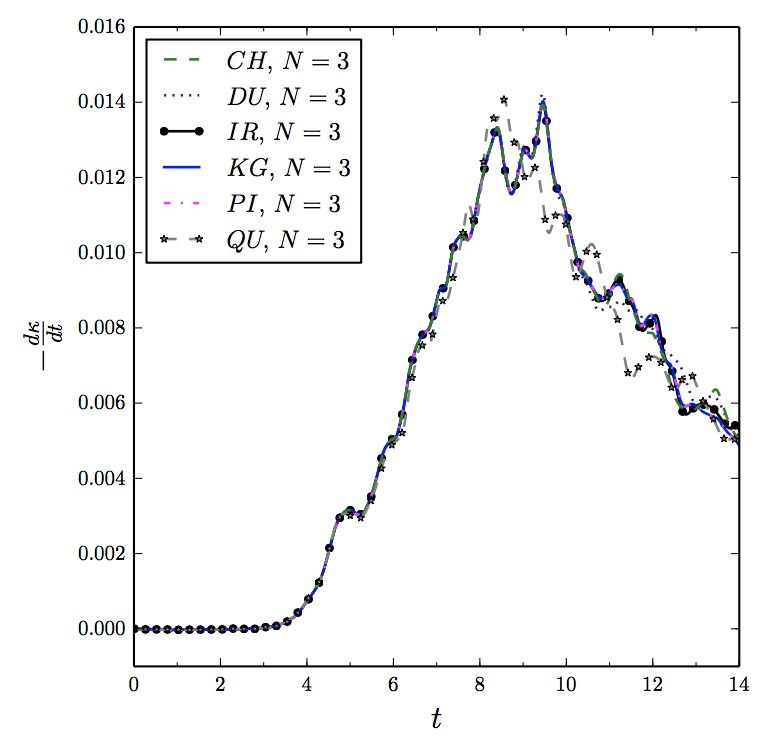
\includegraphics[width=.4\textwidth]{figs/gassner_dkedt.png}
%}
%\hspace{.25em}
%\subfloat[KE dissipation rate]{
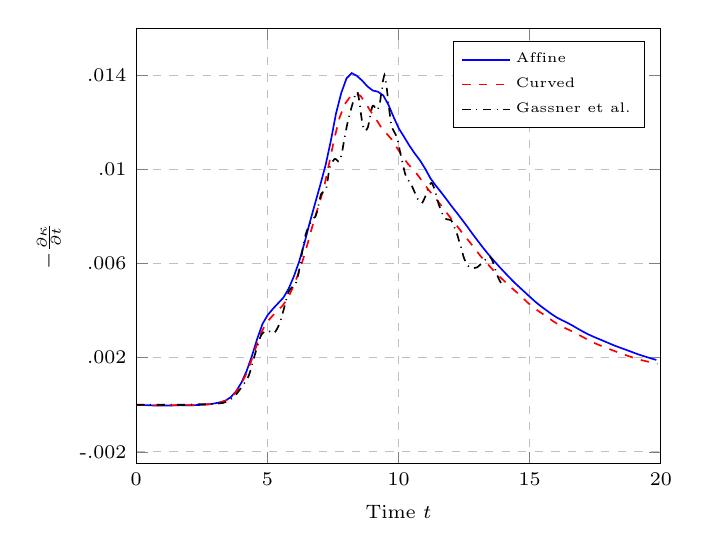
\begin{tikzpicture}
\begin{axis}[
        scaled ticks=false, 
        tick label style={/pgf/number format/fixed},
    legend pos=north east, 
    	legend cell align=left,
	legend style={font=\tiny},        
	width=.68\textwidth,
    xlabel={Time $t$},
    ylabel={$-\pd{\kappa}{t}$},
    xmin=0, xmax=20,
ymin=-.0025, ymax=.016,
    xmajorgrids=true,
    ymajorgrids=true,
    grid style=dashed,
    ytick={-.002,  .002, .006,.01, .014},
    yticklabels={-.002,  .002, .006,.01,   .014}    
] 
\addplot[color=blue,semithick, mark options={fill=markercolor}]
coordinates{(0.007149,-0)(0.207328,-1.12783e-05)(0.407507,-1.46618e-05)(0.607685,-2.53763e-05)(0.807864,-2.98876e-05)(1.00804,-2.65041e-05)(1.20822,-3.15793e-05)(1.4084,-2.48123e-05)(1.60858,-1.97371e-05)(1.80876,-2.42484e-05)(2.00894,-2.0301e-05)(2.20912,-1.40979e-05)(2.40929,-6.767e-06)(2.60947,1.12783e-05)(2.80965,2.98876e-05)(3.00983,6.31587e-05)(3.21001,0.000110528)(3.41019,0.000181581)(3.61037,0.000329891)(3.81054,0.00058027)(4.01072,0.000940613)(4.2109,0.00144081)(4.41108,0.00207803)(4.61126,0.00279816)(4.81144,0.00343031)(5.01162,0.00381377)(5.2118,0.00407881)(5.41197,0.00431791)(5.61215,0.00455532)(5.81233,0.00493822)(6.01251,0.00546492)(6.21269,0.00609087)(6.41287,0.00687415)(6.61305,0.00773299)(6.81323,0.00853827)(7.0134,0.00933057)(7.21358,0.010159)(7.41376,0.0111904)(7.61394,0.0123673)(7.81412,0.0132419)(8.0143,0.013865)(8.21448,0.0140928)(8.41466,0.0139739)(8.61483,0.0137714)(8.81501,0.0135272)(9.01519,0.0133541)(9.21537,0.0133011)(9.41555,0.0131477)(9.61573,0.0127451)(9.81591,0.012215)(10.0161,0.0117295)(10.2163,0.0113731)(10.4164,0.0110065)(10.6166,0.0106795)(10.8168,0.0103857)(11.017,0.0100281)(11.2172,0.00961873)(11.4173,0.00931591)(11.6175,0.00903677)(11.8177,0.0087441)(12.0179,0.00844409)(12.2181,0.00816101)(12.4182,0.0078689)(12.6184,0.00757115)(12.8186,0.00726438)(13.0188,0.00696776)(13.2189,0.00667621)(13.4191,0.00640158)(13.6193,0.00614162)(13.8195,0.0058918)(14.0197,0.00565214)(14.2198,0.00541755)(14.42,0.00519085)(14.6202,0.0049839)(14.8204,0.00477863)(15.0206,0.0045728)(15.2207,0.00437148)(15.4209,0.00419272)(15.6211,0.00402693)(15.8213,0.00386339)(16.0214,0.00371678)(16.2216,0.00359948)(16.4218,0.00349347)(16.622,0.00337222)(16.8222,0.00324083)(17.0223,0.00311451)(17.2225,0.00299835)(17.4227,0.00289571)(17.6229,0.00280323)(17.8231,0.00270906)(18.0232,0.00261432)(18.2234,0.00252071)(18.4236,0.00243612)(18.6238,0.00235717)(18.8239,0.00227371)(19.0241,0.00218913)(19.2243,0.00211187)(19.4245,0.00204025)(19.6247,0.00197089)(19.8248,0.00190548)};

\addplot[color=red, dashed,semithick, mark options={fill=markercolor}]
coordinates{(0.00662,-0)(0.20523,-1.01505e-05)(0.40384,-1.24062e-05)(0.60245,-2.31206e-05)(0.801059,-2.59402e-05)(0.999669,-2.31206e-05)(1.19828,-2.81958e-05)(1.39689,-2.19928e-05)(1.5955,-1.80453e-05)(1.79411,-2.14288e-05)(1.99272,-1.86093e-05)(2.19133,-1.63536e-05)(2.38994,-8.45875e-06)(2.58855,5.07525e-06)(2.78716,2.0301e-05)(2.98577,4.96247e-05)(3.18438,9.4738e-05)(3.38299,0.000160152)(3.5816,0.000283086)(3.78021,0.000504706)(3.97881,0.000825574)(4.17743,0.00126543)(4.37603,0.00183499)(4.57464,0.00247672)(4.77325,0.0030897)(4.97186,0.00349741)(5.17047,0.00375061)(5.36908,0.00398971)(5.56769,0.00419893)(5.7663,0.00449555)(5.96491,0.00496811)(6.16352,0.00551849)(6.36213,0.00618335)(6.56074,0.00695535)(6.75935,0.00776796)(6.95796,0.00847567)(7.15657,0.00922568)(7.35518,0.0102655)(7.55379,0.0113212)(7.7524,0.0122049)(7.95101,0.0127772)(8.14962,0.0130801)(8.34823,0.0132329)(8.54684,0.0131302)(8.74545,0.012815)(8.94406,0.0124564)(9.14267,0.0121327)(9.34128,0.0117836)(9.53989,0.0115276)(9.7385,0.0112761)(9.93711,0.0109236)(10.1357,0.0105819)(10.3343,0.0102689)(10.5329,0.0100225)(10.7315,0.00976309)(10.9302,0.00945689)(11.1288,0.00915857)(11.3274,0.00887436)(11.526,0.00861327)(11.7246,0.00831947)(11.9232,0.00802623)(12.1218,0.00775273)(12.3204,0.00746513)(12.519,0.00717584)(12.7176,0.00690742)(12.9163,0.00662038)(13.1149,0.00633448)(13.3135,0.00608184)(13.5121,0.00583767)(13.7107,0.00559631)(13.9093,0.00538653)(14.1079,0.00517958)(14.3065,0.00497093)(14.5051,0.00477976)(14.7037,0.00457393)(14.9024,0.00436246)(15.101,0.00417242)(15.2996,0.00400832)(15.4982,0.00385719)(15.6968,0.00370663)(15.8954,0.00355042)(16.094,0.00340831)(16.2926,0.00329102)(16.4912,0.00318557)(16.6898,0.00307729)(16.8884,0.00296056)(17.0871,0.00284214)(17.2857,0.00272597)(17.4843,0.00261714)(17.6829,0.00252353)(17.8815,0.00243725)(18.0801,0.00234984)(18.2787,0.00226413)(18.4773,0.00218349)(18.6759,0.0021051)(18.8745,0.00202954)(19.0732,0.00195848)(19.2718,0.00189589)(19.4704,0.00184288)(19.669,0.00179438)(19.8676,0.00174476)};

\addplot[smooth,color=black,dashdotted,semithick, mark options={solid,fill=markercolor}]
  coordinates{(0.0,0) (0.28719,0) (0.53378,0) (0.78906,0) (1.04434,0) (1.29963,0) (1.54041,0) (1.80439,0) (2.05097,6.28e-06) (2.29755,2.197e-05) (2.54994,2.51e-05) (2.79942,2.51e-05) (3.0518,5.334e-05) (3.30709,7.845e-05) (3.54206,0.00019141) (3.80025,0.00042989) (4.04112,0.00079443) (4.28761,0.00123005) (4.53129,0.00216199) (4.76046,0.00295274) (5.00705,0.0031567) (5.25073,0.00304373) (5.4857,0.00352069) (5.73518,0.0045405) (5.75839,0.00465815) (5.82703,0.0048383) (5.90054,0.00495156) (5.97306,0.00503628) (6.03978,0.00505511) (6.08399,0.0051618) (6.20804,0.00570151) (6.43722,0.00715434) (6.7041,0.0078635) (6.82884,0.00798902) (6.91587,0.00831222) (7.04932,0.00895862) (7.18856,0.00906844) (7.25238,0.00924417) (7.2988,0.00955481) (7.33941,0.00986546) (7.40033,0.01016356) (7.57149,0.01044911) (7.73394,0.01032987) (7.83838,0.01067503) (7.88479,0.01098255) (7.93701,0.01129633) (7.98632,0.01160384) (8.10816,0.01222828) (8.33444,0.01312257) (8.42884,0.01330112) (8.46259,0.0131414) (8.49792,0.0129375) (8.61293,0.01200549) (8.68835,0.01169798) (8.70286,0.01164464) (8.8305,0.01179212) (9.01027,0.01269896) (9.1776,0.01250441) (9.28595,0.01280565) (9.32366,0.01310688) (9.37298,0.01343008) (9.40199,0.0137376) (9.46291,0.01401373) (9.49482,0.01383173) (9.54414,0.01352108) (9.59055,0.0130504) (9.65727,0.0124291) (9.7385,0.01182663) (9.92706,0.01139674) (9.99668,0.01108296) (10.08661,0.01059345) (10.20845,0.01000981) (10.23746,0.00986233) (10.3448,0.00955795) (10.43763,0.00946695) (10.50435,0.0093132) (10.67261,0.00888017) (10.73063,0.00874211) (10.88438,0.00856952) (11.02362,0.00886135) (11.11935,0.00918141) (11.2528,0.0094293) (11.37754,0.00914689) (11.45006,0.00885507) (11.52549,0.00853501) (11.62122,0.00824946) (11.73436,0.00795136) (11.84169,0.00787919) (12.00995,0.0078384) (12.11148,0.00757796) (12.21881,0.00729555) (12.30004,0.00698804) (12.38417,0.00668994) (12.45379,0.00638243) (12.54372,0.00609688) (12.72068,0.00583644) (12.97596,0.00583016) (13.20514,0.00605609) (13.2963,0.0061533) (13.42754,0.00631269) (13.54745,0.00619729) (13.64608,0.00590233) (13.73021,0.00559796) (13.84045,0.00530928) (13.97389,0.00503314) (13.9913,0.00499504)};

 
\legend{Affine, Curved, Gassner et al.}% , Beck et al.\ (viscous), Spectral (viscous)}
\end{axis}\end{tikzpicture}
%}
}
%\caption{Evolution of kinetic energy $\kappa(t)$ and kinetic energy dissipation rate $-\pd{\kappa}{t}$ for $N=3, h = \pi/8, \text{CFL} = .25$ on affine and curved meshes.}
\caption*{Kinetic energy dissipation rate $-\pd{\kappa}{t}$ for $N=3, h = \pi/8, \text{CFL} = .25$ (tet meshes).}% on affine and curved meshes.}
\end{figure}

}

\subsection{Quadrilateral and hexahedral meshes}

\frame[noframenumbering]{
\frametitle{Talk outline}
\tableofcontents[currentsection,currentsubsection]
}


\frame{
\frametitle{Entropy stable Gauss collocation: main steps}
\begin{columns}
\hspace{-.5em}
\begin{column}{.49\textwidth}
\vspace{-.5em}
\begin{figure}
\centering
\begin{overlayarea}{.75\textwidth}{.425\textheight}
\only<1>{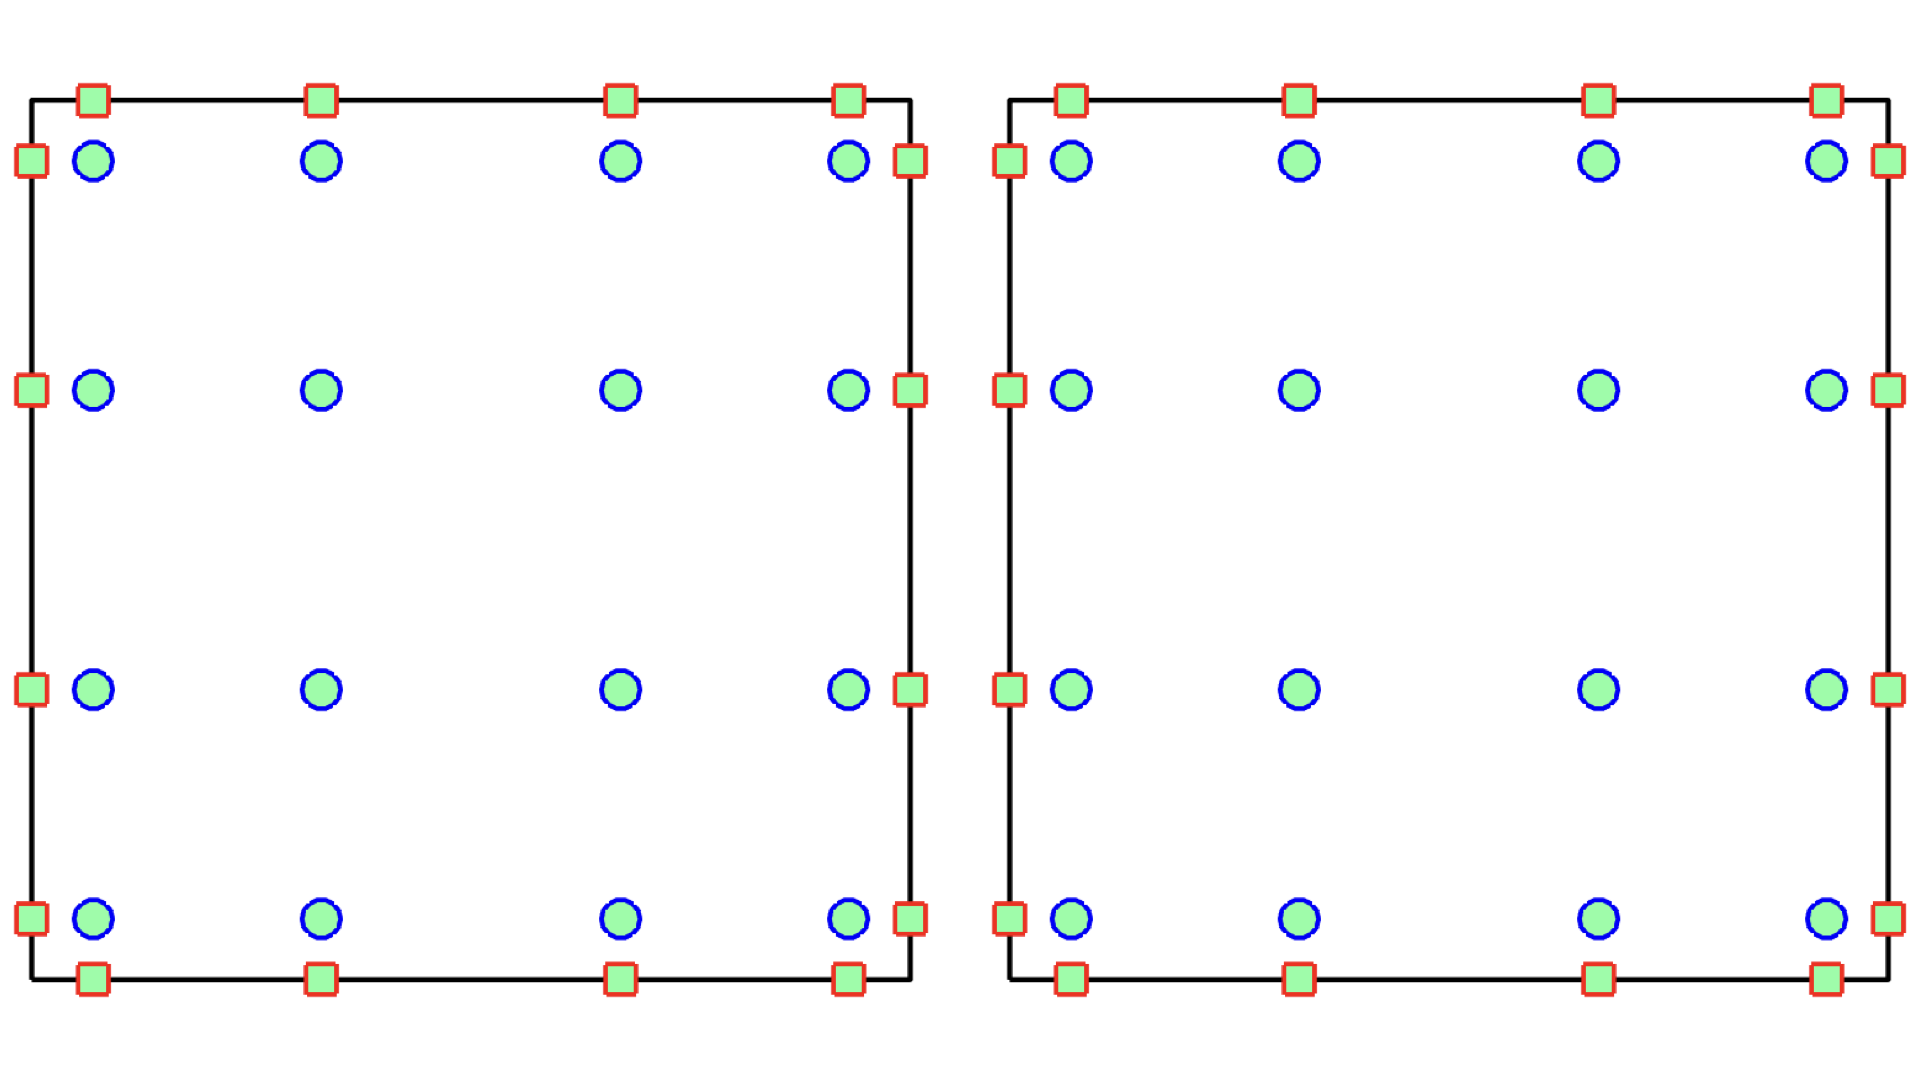
\includegraphics[height=.425\textheight]{figs/gsbp1.png}}
\only<2>{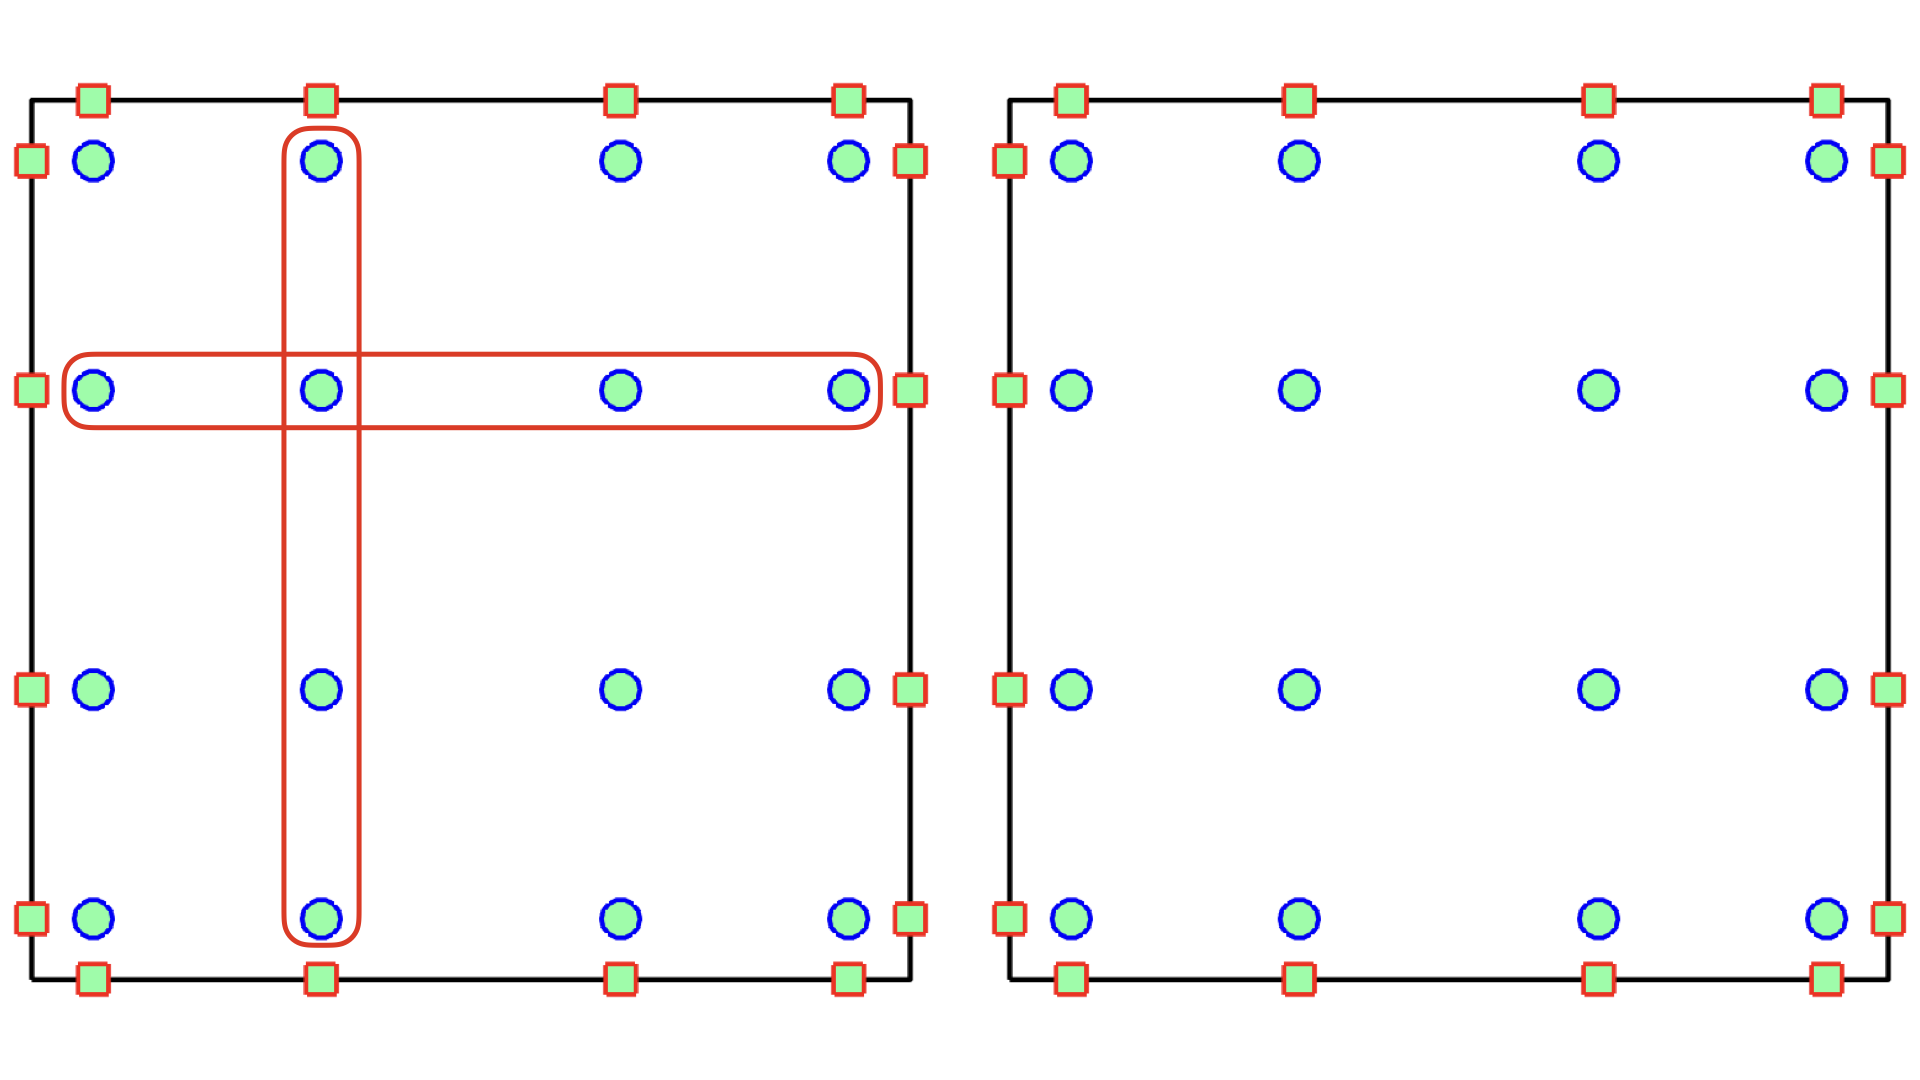
\includegraphics[height=.425\textheight]{figs/gsbp2.png}}
\only<3>{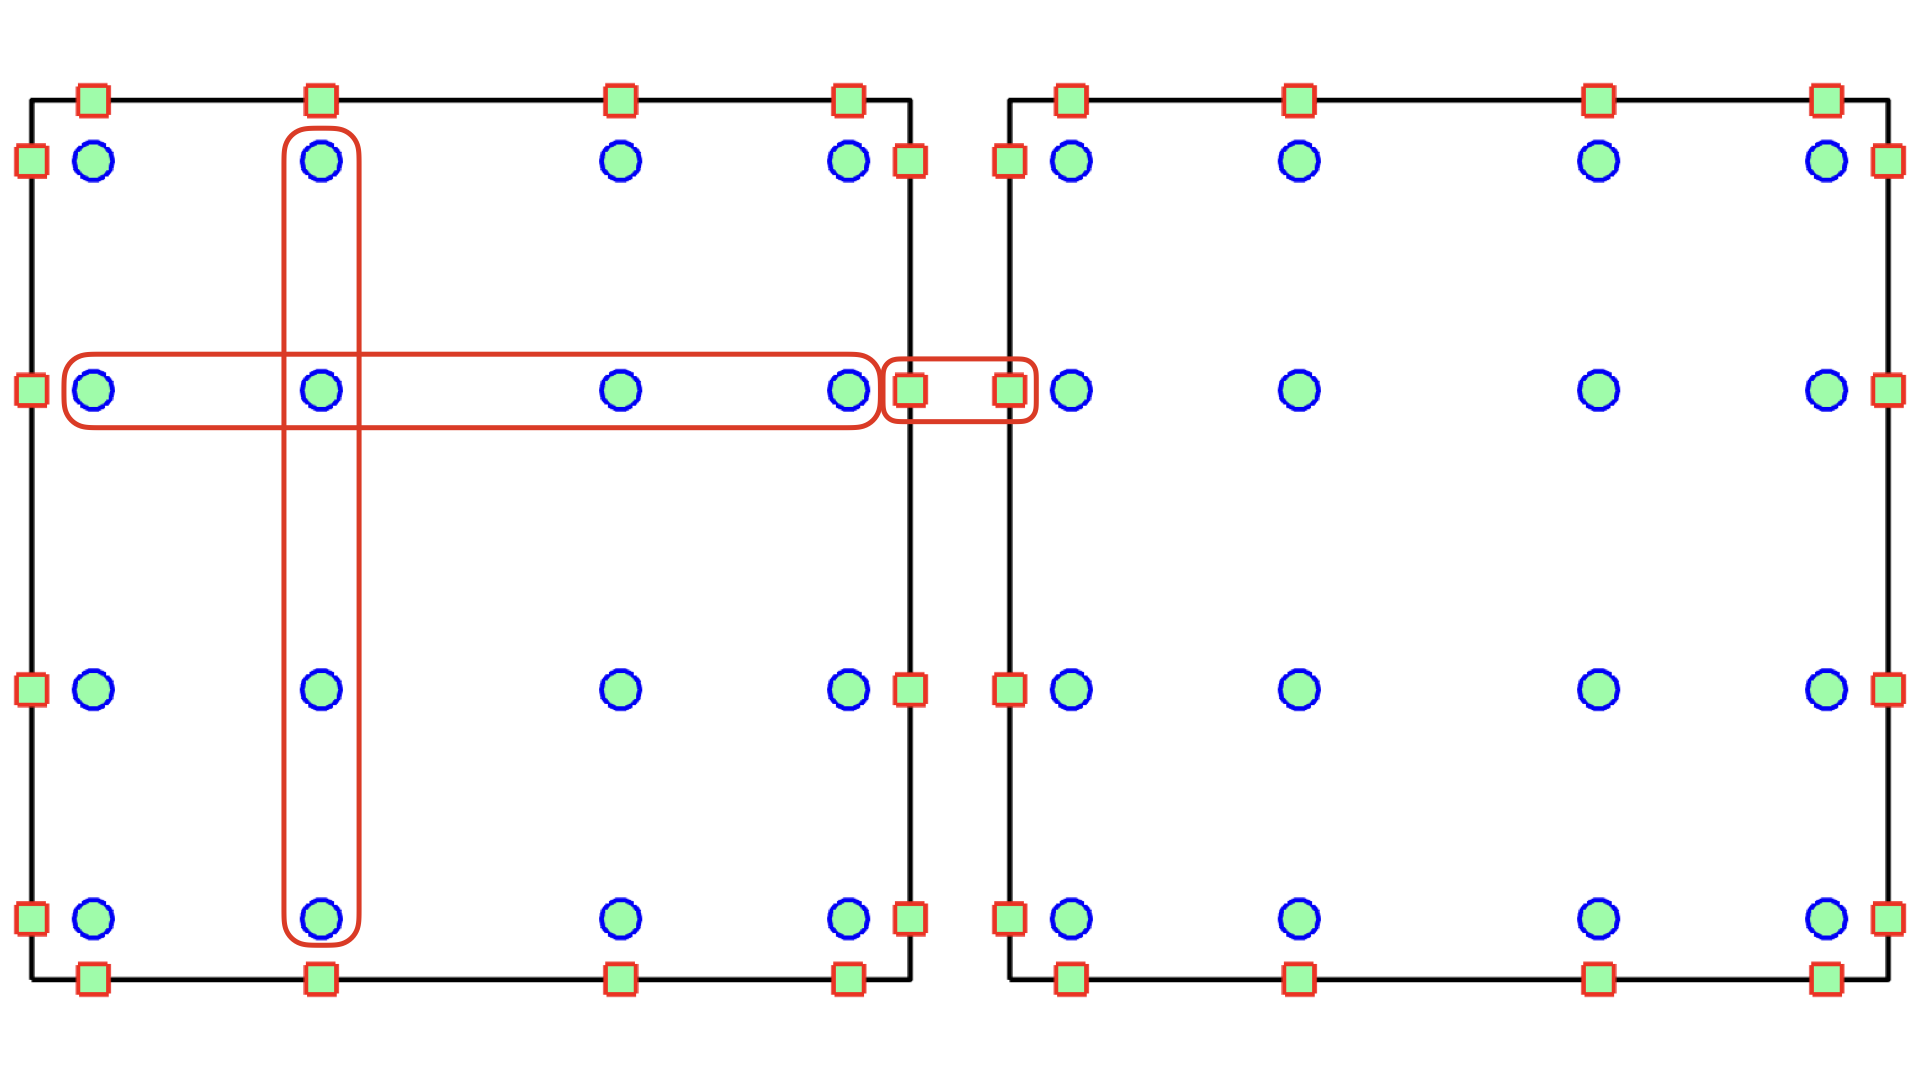
\includegraphics[height=.425\textheight]{figs/gsbp3.png}}
\only<4>{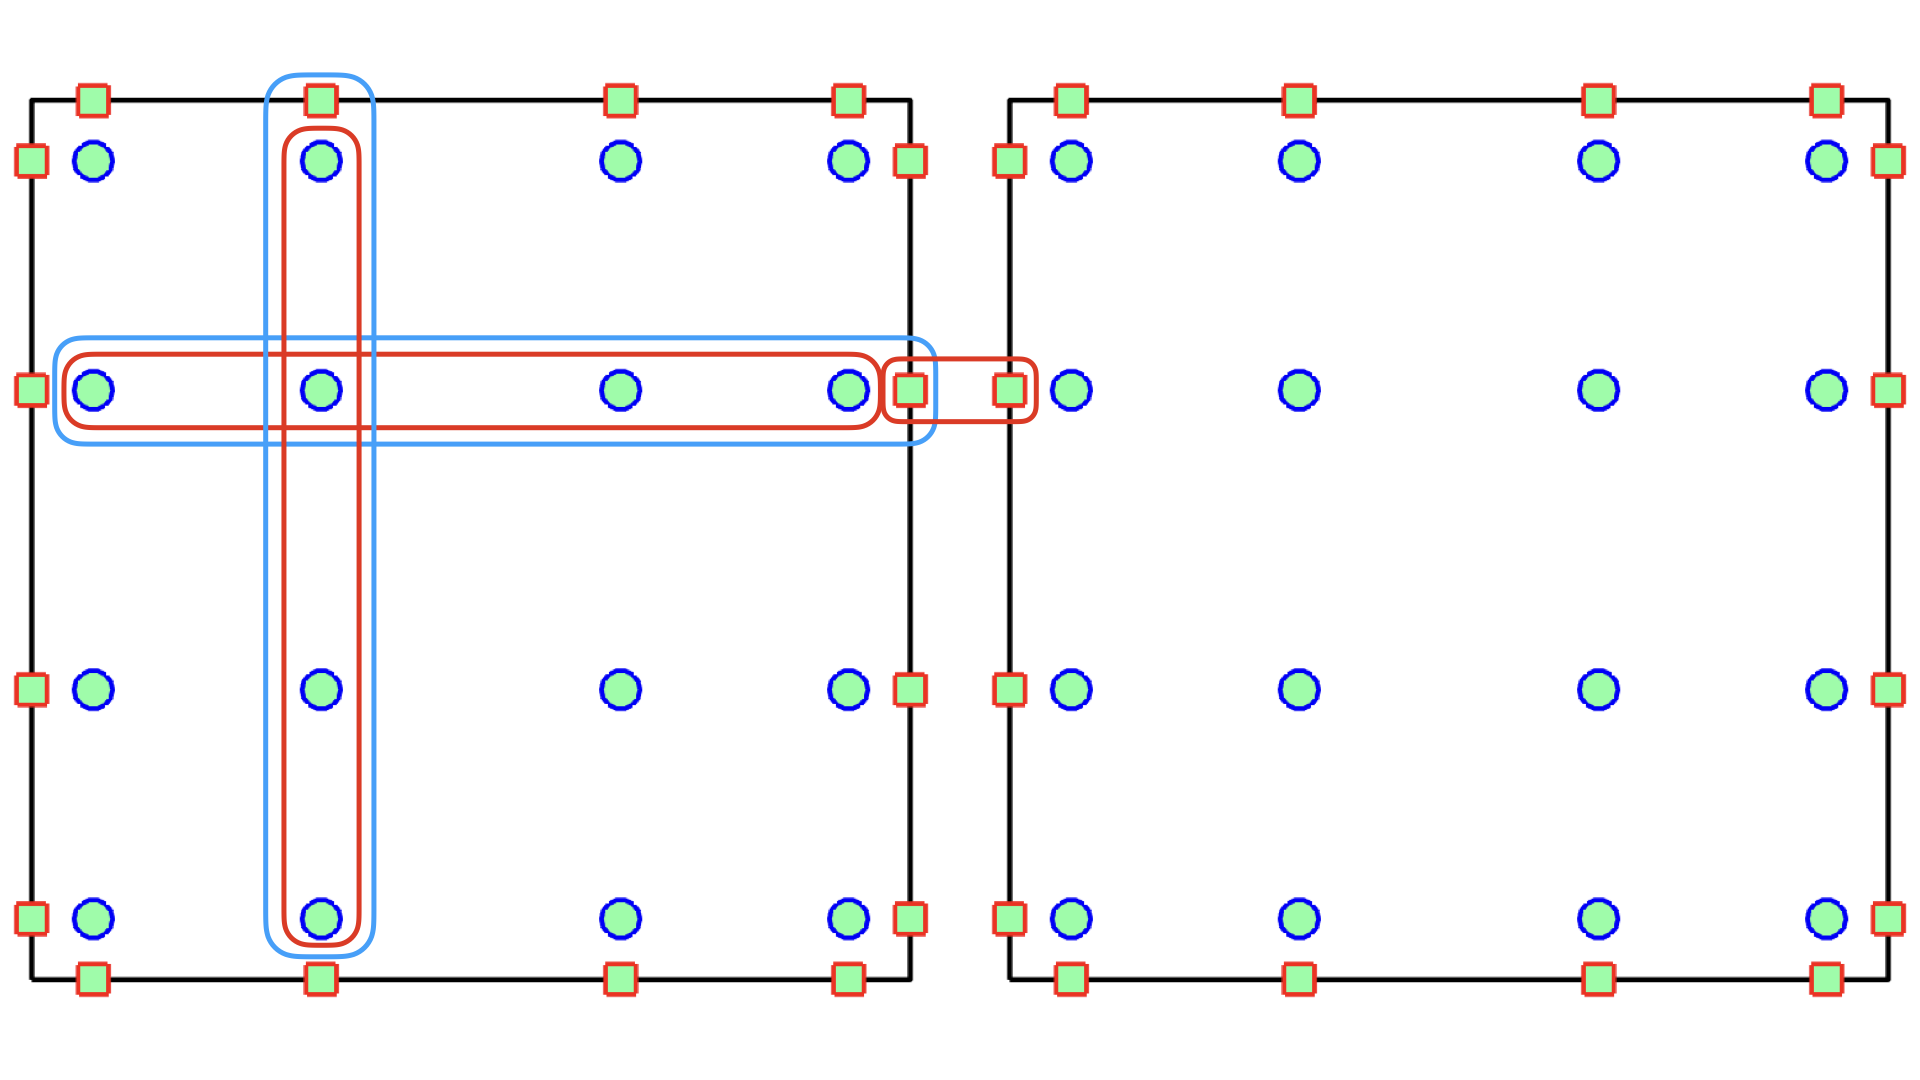
\includegraphics[height=.425\textheight]{figs/gsbp4.png}}
%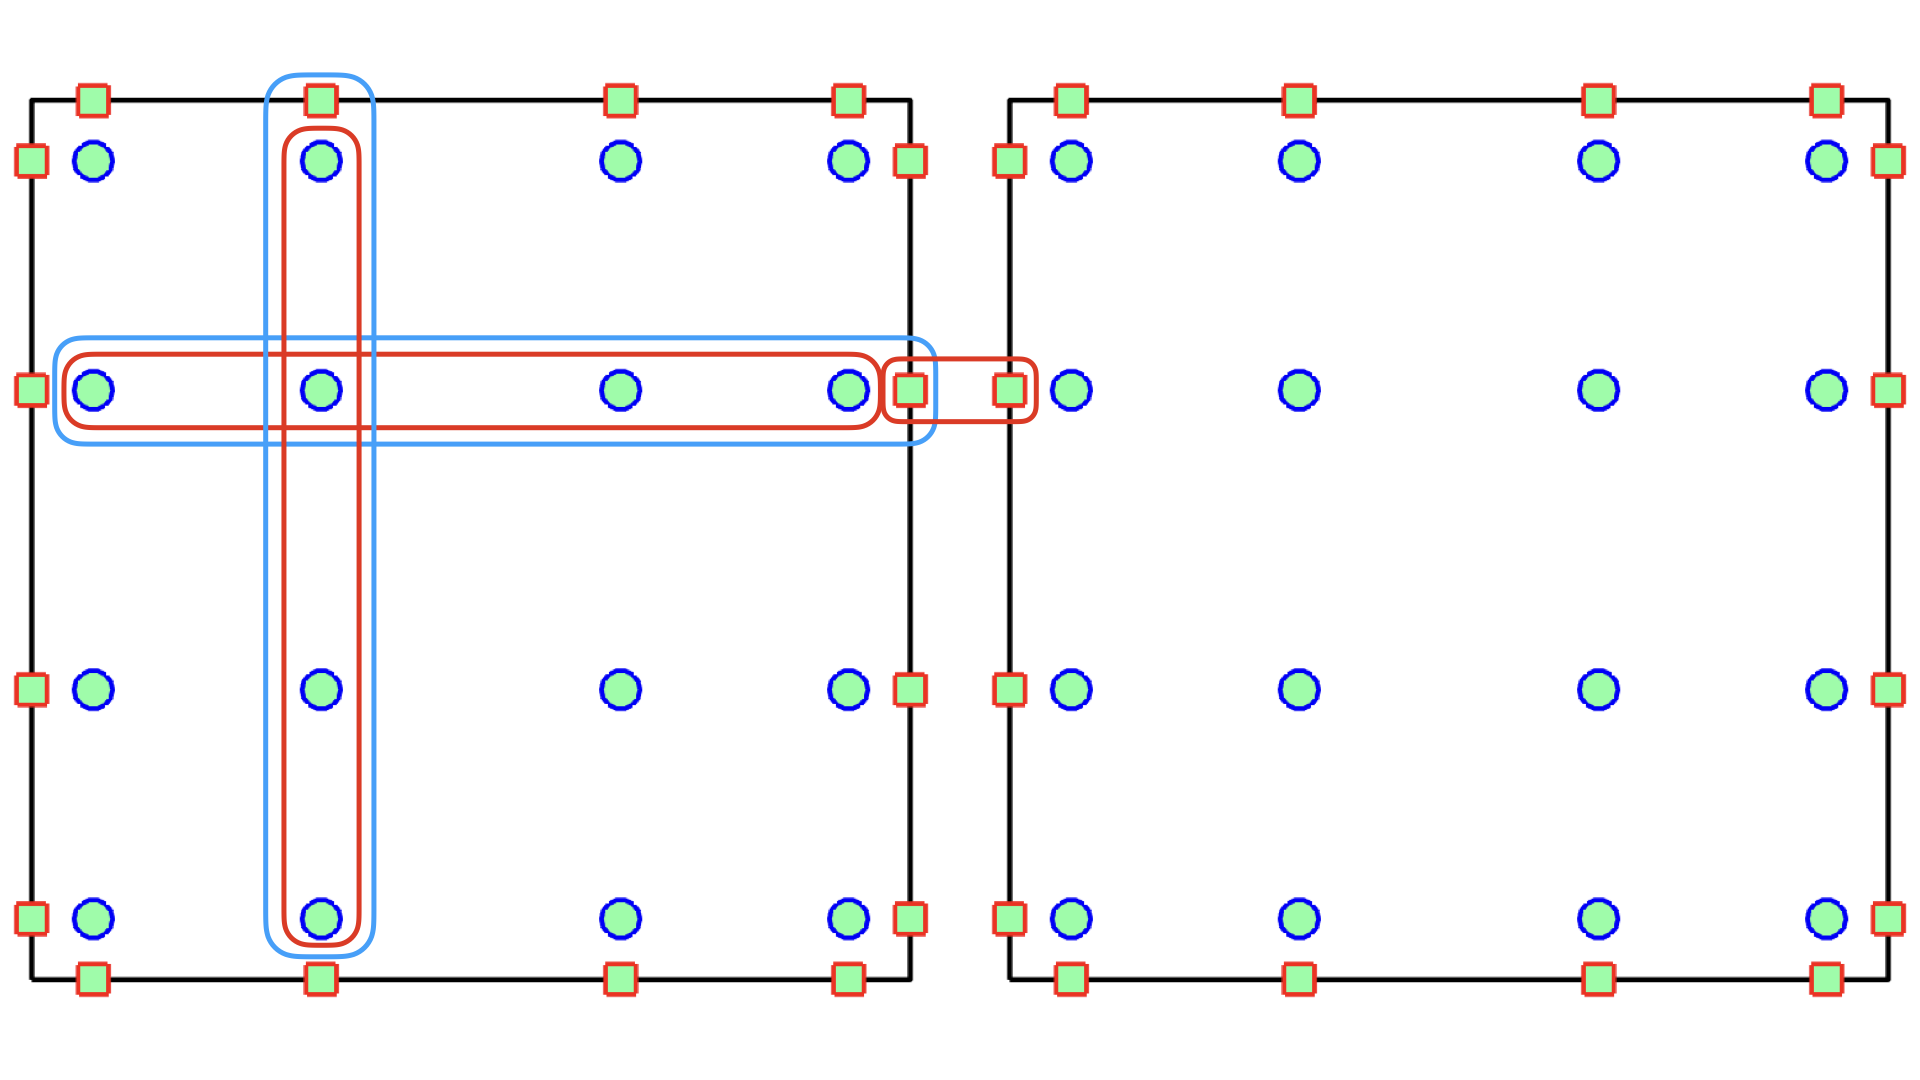
\includegraphics[height=.45\textheight]{figs/gsbp4.png}
\end{overlayarea}
\end{figure}
\end{column}
%\vspace{-2.5em}
\hspace{3em}
\begin{column}{.51\textwidth}
\[
\only<1>{
\LRp{\underbrace{\begin{bmatrix}
\bm{A} & \bm{B}\\
-\bm{B}^T & \bm{C}
\end{bmatrix}}_{\bm{Q}_N^i} \circ
\underbrace{\begin{bmatrix}
\bm{F}^{vv}_S & \bm{F}^{vf}_S\\
\bm{F}^{fv}_S & \bm{F}^{ff}_S
\end{bmatrix}}_{\bm{F}_S} } \bm{1}
}
\only<2>{
\LRp{\underbrace{\begin{bmatrix}
\note{\bm{A}} & \bm{B}\\
-\bm{B}^T & \bm{C}
\end{bmatrix}}_{\bm{Q}_N^i} \circ
\underbrace{\begin{bmatrix}
\note{\bm{F}^{vv}_S} & \bm{F}^{vf}_S\\
\bm{F}^{fv}_S & \bm{F}^{ff}_S
\end{bmatrix}}_{\bm{F}_S} } \bm{1}
}
\only<3>{
\LRp{\underbrace{\begin{bmatrix}
\bm{A} & \bm{B}\\
-\bm{B}^T & \note{\bm{C}}
\end{bmatrix}}_{\bm{Q}_N^i} \circ
\underbrace{\begin{bmatrix}
\bm{F}^{vv}_S & \bm{F}^{vf}_S\\
\bm{F}^{fv}_S & \note{\bm{F}^{ff}_S}
\end{bmatrix}}_{\bm{F}_S} } \bm{1}
}
\only<4>{
\LRp{\underbrace{\begin{bmatrix}
\bm{A} & \note{\bm{B}}\\
\note{-\bm{B}^T} & \bm{C}
\end{bmatrix}}_{\bm{Q}_N^i} \circ
\underbrace{\begin{bmatrix}
\bm{F}^{vv}_S & \note{\bm{F}^{vf}_S}\\
\note{\bm{F}^{fv}_S} & \bm{F}^{ff}_S
\end{bmatrix}}_{\bm{F}_S} } \bm{1}
}
\]
\end{column}
\end{columns}
\vspace{.5em}
\begin{itemize}
\item Advantage of hexahedra vs.\ tetrahedra: tensor product structure.
\vspace{.5em}
\item $(N+1)$-point Gauss quadrature reduces to a \note{collocation scheme}.  
\vspace{.5em}
\item Reduces computational costs from $O(N^6)$ to $O(N^4)$ in 3D.
\vspace{.5em}
\end{itemize} 
}


\frame{
\frametitle{Gauss quadrature improves errors on curved meshes}

\begin{figure}
\centering
\begin{overlayarea}{\textwidth}{.55\textheight}
\only<1>{
\raisebox{3.5em}{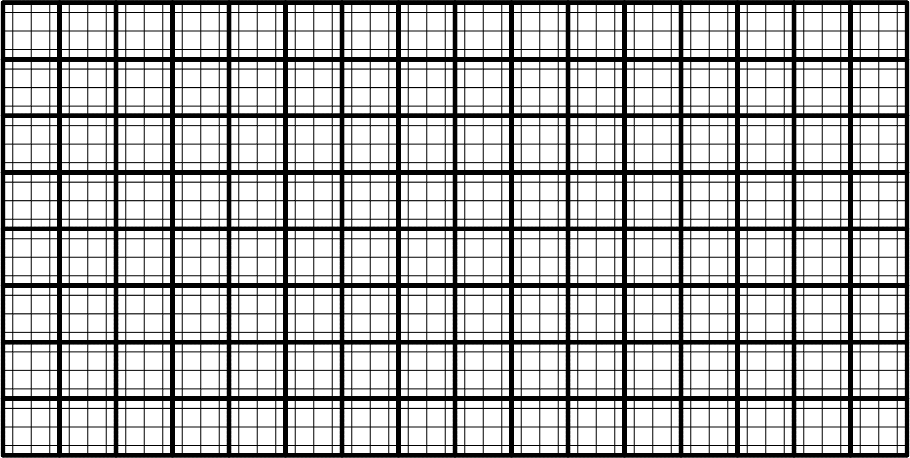
\includegraphics[width=.475\textwidth]{figs/warp2d_a0.png}}
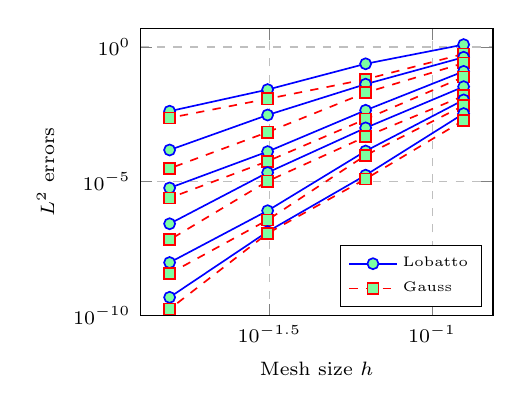
\begin{tikzpicture}
\begin{loglogaxis}[
    width=.5\textwidth,
    xlabel={Mesh size $h$},
    ylabel={$L^2$ errors}, 
%    xmin=.0125, 
    ymin=1e-10, ymax=5,
    legend pos=south east, legend cell align=left, legend style={font=\tiny},	
    xmajorgrids=true, ymajorgrids=true, grid style=dashed,
    legend entries={Lobatto, Gauss}    
]
\pgfplotsset{
cycle list={{blue, mark=*}, {red, dashed ,mark=square*}}
}
\addplot+[semithick, mark options={solid, fill=markercolor}]
coordinates{(0.125,1.22861)(0.0625,0.236646)(0.03125,0.0258883)(0.015625,0.00406122)};
\addplot+[semithick, mark options={solid, fill=markercolor}]
coordinates{(0.125,0.553435)(0.0625,0.0625441)(0.03125,0.0117156)(0.015625,0.0022841)}; %(0.0078125,0.000362526)

\addplot+[semithick, mark options={solid, fill=markercolor}]
coordinates{(0.125,0.414449)(0.0625,0.0412224)(0.03125,0.00293039)(0.015625,0.000145701)};
\addplot+[semithick, mark options={solid, fill=markercolor}]
coordinates{(0.125,0.25082)(0.0625,0.0198863)(0.03125,0.000673152)(0.015625,2.98263e-05)}; %(0.0078125, 1.77421e-06)

\addplot+[semithick, mark options={solid, fill=markercolor}]
coordinates{(0.125,0.123516)(0.0625,0.00439285)(0.03125,0.000126852)(0.015625,5.61786e-06)};
\addplot+[semithick, mark options={solid, fill=markercolor}]
coordinates{(0.125,0.0768018)(0.0625,0.0020579)(0.03125,5.55322e-05)(0.015625,2.36108e-06)}; % (0.0078125,8.55848e-08)

\addplot+[semithick, mark options={solid, fill=markercolor}]
coordinates{(0.125,0.0332509)(0.0625,0.000970148)(0.03125,2.10334e-05)(0.015625,2.60008e-07)};
\addplot+[semithick, mark options={solid, fill=markercolor}]
coordinates{(0.125,0.0151231)(0.0625,0.000454595)(0.03125,1.00203e-05)(0.015625,6.57796e-08)}; %(0.0078125, 9.32809e-10)

\addplot+[semithick, mark options={solid, fill=markercolor}]
coordinates{(0.125,0.0106752)(0.0625,0.000133284)(0.03125,7.97032e-07)(0.015625,9.35152e-09)};
\addplot+[semithick, mark options={solid, fill=markercolor}]
coordinates{(0.125,0.00657096)(0.0625,9.22845e-05)(0.03125,3.60025e-07)(0.015625,3.63974e-09)}; %(0.0078125, 1.23726e-10)

\addplot+[semithick, mark options={solid, fill=markercolor}]
coordinates{(0.125,0.00330917)(0.0625,1.67825e-05)(0.03125,1.32696e-07)(0.015625,4.73518e-10)};
\addplot+[semithick, mark options={solid, fill=markercolor}]
coordinates{(0.125,0.00185273)(0.0625,1.21465e-05)(0.03125,1.14289e-07)(0.015625,1.72358e-10)}; 

\end{loglogaxis}
\end{tikzpicture}
}
\only<2>{
\raisebox{3.5em}{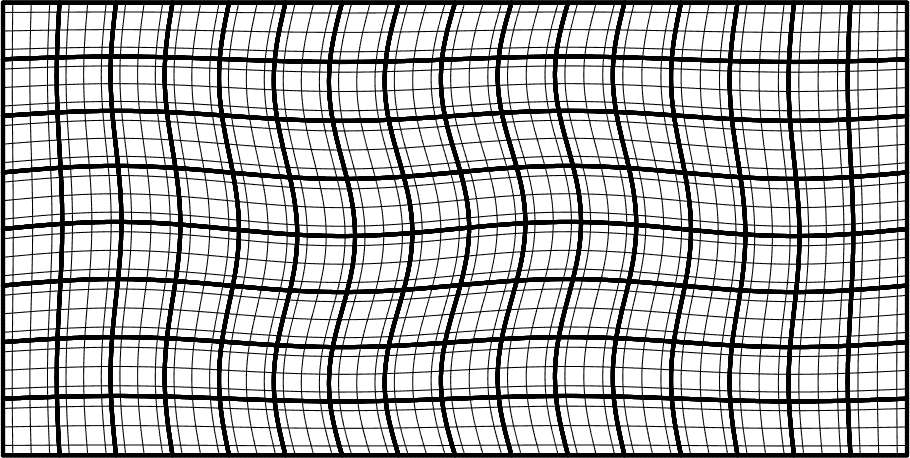
\includegraphics[width=.475\textwidth]{figs/warp2d_a0312.png}}
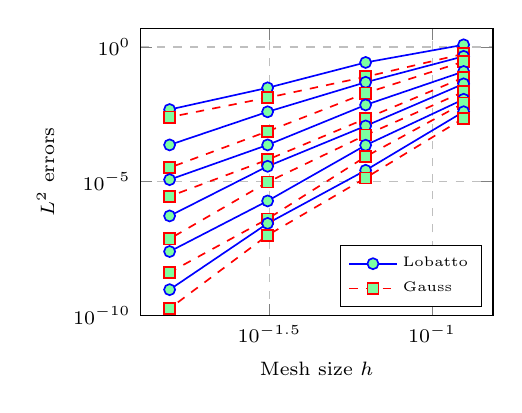
\begin{tikzpicture}
\begin{loglogaxis}[
    width=.5\textwidth,
    xlabel={Mesh size $h$},
    ylabel={$L^2$ errors}, 
%    xmin=.0125, 
    ymin=1e-10, ymax=5,
    legend pos=south east, legend cell align=left, legend style={font=\tiny},	
    xmajorgrids=true, ymajorgrids=true, grid style=dashed,
    legend entries={Lobatto, Gauss}    
]
\pgfplotsset{
cycle list={{blue, mark=*}, {red, dashed ,mark=square*}}
}
\addplot+[semithick, mark options={solid, fill=markercolor}]
coordinates{(0.125,1.2082)(0.0625,0.265357)(0.03125,0.0301118)(0.015625,0.00467693)};
\addplot+[semithick, mark options={solid, fill=markercolor}]
coordinates{(0.125,0.555586)(0.0625,0.0773534)(0.03125,0.0129171)(0.015625,0.0024363)};
\addplot+[semithick, mark options={solid, fill=markercolor}]
coordinates{(0.125,0.448878)(0.0625,0.0485323)(0.03125,0.00385418)(0.015625,0.000225396)};
\addplot+[semithick, mark options={solid, fill=markercolor}]
coordinates{(0.125,0.287685)(0.0625,0.0190431)(0.03125,0.000721055)(0.015625,3.19095e-05)};
\addplot+[semithick, mark options={solid, fill=markercolor}]
coordinates{(0.125,0.122081)(0.0625,0.00694351)(0.03125,0.000224524)(0.015625,1.14555e-05)};
\addplot+[semithick, mark options={solid, fill=markercolor}]
coordinates{(0.125,0.0731583)(0.0625,0.00213914)(0.03125,6.32128e-05)(0.015625,2.73037e-06)};
\addplot+[semithick, mark options={solid, fill=markercolor}]
coordinates{(0.125,0.0424351)(0.0625,0.00114569)(0.03125,3.59697e-05)(0.015625,5.09643e-07)};
\addplot+[semithick, mark options={solid, fill=markercolor}]
coordinates{(0.125,0.0215298)(0.0625,0.000523714)(0.03125,9.27521e-06)(0.015625,7.14031e-08)};
\addplot+[semithick, mark options={solid, fill=markercolor}]
coordinates{(0.125,0.0112838)(0.0625,0.000219049)(0.03125,1.84304e-06)(0.015625,2.40402e-08)};
\addplot+[semithick, mark options={solid, fill=markercolor}]
coordinates{(0.125,0.00809138)(0.0625,8.23415e-05)(0.03125,3.95565e-07)(0.015625,4.01268e-09)};
\addplot+[semithick, mark options={solid, fill=markercolor}]
coordinates{(0.125,0.00388316)(0.0625,2.55074e-05)(0.03125,2.68102e-07)(0.015625,9.13754e-10)};
\addplot+[semithick, mark options={solid, fill=markercolor}]
coordinates{(0.125,0.00222029)(0.0625,1.33111e-05)(0.03125,9.72405e-08)(0.015625,1.81386e-10)};

\end{loglogaxis}
\end{tikzpicture}
}
\only<3>{
\raisebox{3.5em}{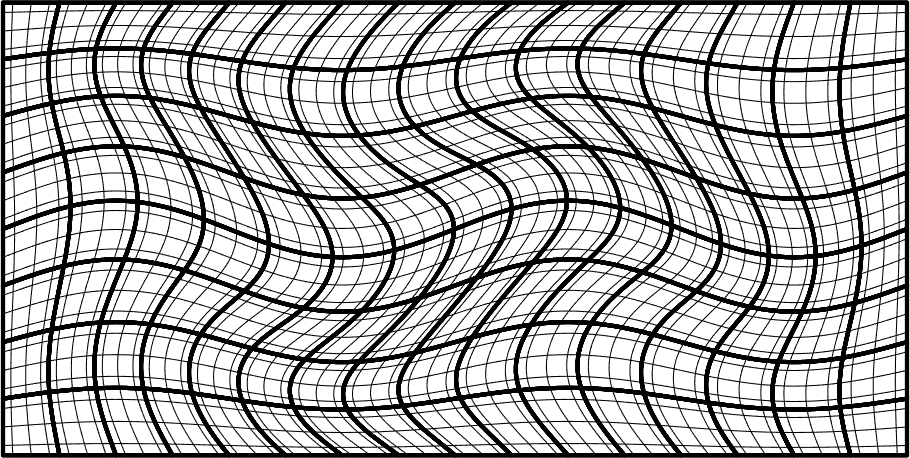
\includegraphics[width=.475\textwidth]{figs/warp2d_a125.png}}
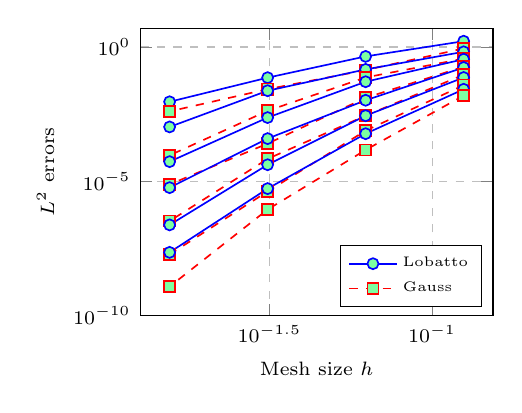
\begin{tikzpicture}
\begin{loglogaxis}[
    width=.5\textwidth,
    xlabel={Mesh size $h$},
    ylabel={$L^2$ errors}, 
%    xmin=.0125,
    ymin=1e-10, ymax=5,
    legend pos=south east, legend cell align=left, legend style={font=\tiny},	
    xmajorgrids=true, ymajorgrids=true, grid style=dashed,
    legend entries={Lobatto, Gauss}    
]
\pgfplotsset{
cycle list={{blue, mark=*}, {red, dashed ,mark=square*}}
}
\addplot+[semithick, mark options={solid, fill=markercolor}]
coordinates{(0.125,1.64274)(0.0625,0.445945)(0.03125,0.0720148)(0.015625,0.0091066)};
\addplot+[semithick, mark options={solid, fill=markercolor}]
coordinates{(0.125,0.882247)(0.0625,0.138116)(0.03125,0.0268145)(0.015625,0.0039945)};
\addplot+[semithick, mark options={solid, fill=markercolor}]
coordinates{(0.125,0.662165)(0.0625,0.146131)(0.03125,0.0234934)(0.015625,0.00105368)};
\addplot+[semithick, mark options={solid, fill=markercolor}]
coordinates{(0.125,0.368084)(0.0625,0.0734059)(0.03125,0.00420438)(0.015625,9.19378e-05)};
\addplot+[semithick, mark options={solid, fill=markercolor}]
coordinates{(0.125,0.349184)(0.0625,0.0508268)(0.03125,0.00234785)(0.015625,5.36192e-05)};
\addplot+[semithick, mark options={solid, fill=markercolor}]
coordinates{(0.125,0.183472)(0.0625,0.0127617)(0.03125,0.000251929)(0.015625,7.6013e-06)};
\addplot+[semithick, mark options={solid, fill=markercolor}]
coordinates{(0.125,0.171986)(0.0625,0.0103578)(0.03125,0.000386834)(0.015625,5.76284e-06)};
\addplot+[semithick, mark options={solid, fill=markercolor}]
coordinates{(0.125,0.0924215)(0.0625,0.00276519)(0.03125,6.80528e-05)(0.015625,3.27246e-07)};
\addplot+[semithick, mark options={solid, fill=markercolor}]
coordinates{(0.125,0.0729963)(0.0625,0.00276104)(0.03125,4.11305e-05)(0.015625,2.36125e-07)};
\addplot+[semithick, mark options={solid, fill=markercolor}]
coordinates{(0.125,0.0378013)(0.0625,0.0007649)(0.03125,4.15848e-06)(0.015625,1.8685e-08)};
\addplot+[semithick, mark options={solid, fill=markercolor}]
coordinates{(0.125,0.026577)(0.0625,0.000589552)(0.03125,5.3039e-06)(0.015625,2.23719e-08)};
\addplot+[semithick, mark options={solid, fill=markercolor}]
coordinates{(0.125,0.0154563)(0.0625,0.000146207)(0.03125,8.83156e-07)(0.015625,1.18829e-09)};

\end{loglogaxis}
\end{tikzpicture}
}
\only<4>{
\raisebox{3.5em}{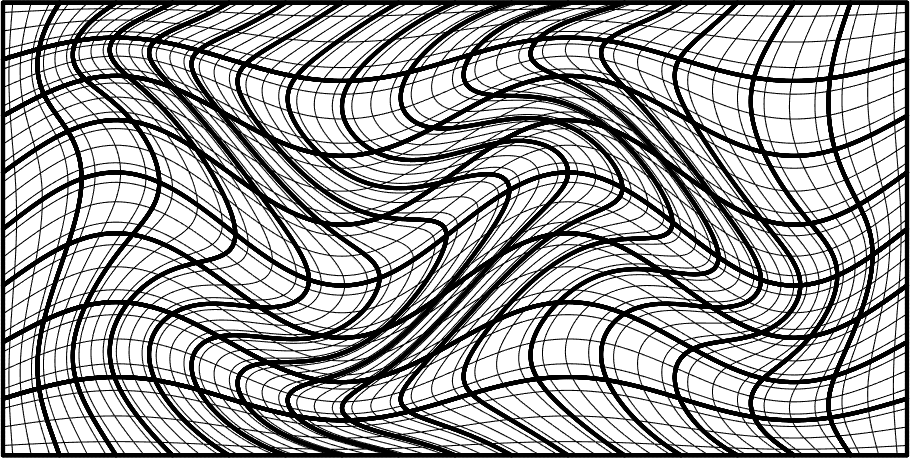
\includegraphics[width=.475\textwidth]{figs/warp2d_a25.png}}
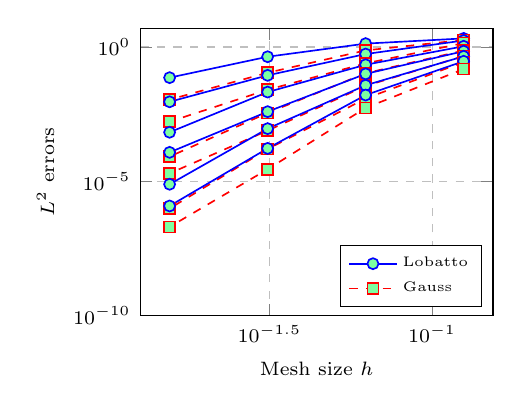
\begin{tikzpicture}
\begin{loglogaxis}[
    width=.5\textwidth,
    xlabel={Mesh size $h$},
    ylabel={$L^2$ errors}, 
%    xmin=.0125,
    ymin=1e-10, ymax=5,
    legend pos=south east, legend cell align=left, legend style={font=\tiny},	
    xmajorgrids=true, ymajorgrids=true, grid style=dashed,
    legend entries={Lobatto, Gauss}    
]
\pgfplotsset{
cycle list={{blue, mark=*}, {red, dashed ,mark=square*}}
}
\addplot+[semithick, mark options={solid, fill=markercolor}]
coordinates{(0.125,2.08578)(0.0625,1.33668)(0.03125,0.433653)(0.015625,0.0721002)};
\addplot+[semithick, mark options={solid, fill=markercolor}]
coordinates{(0.125,1.82833)(0.0625,0.746283)(0.03125,0.11006)(0.015625,0.0110115)};
\addplot+[semithick, mark options={solid, fill=markercolor}]
coordinates{(0.125,1.74649)(0.0625,0.546097)(0.03125,0.0879841)(0.015625,0.0090851)};
\addplot+[semithick, mark options={solid, fill=markercolor}]
coordinates{(0.125,1.39268)(0.0625,0.245852)(0.03125,0.0255562)(0.015625,0.00165226)};
\addplot+[semithick, mark options={solid, fill=markercolor}]
coordinates{(0.125,1.06289)(0.0625,0.218361)(0.03125,0.0209471)(0.015625,0.000665425)};
\addplot+[semithick, mark options={solid, fill=markercolor}]
coordinates{(0.125,0.740071)(0.0625,0.105075)(0.03125,0.003505)(0.015625,8.26421e-05)};
\addplot+[semithick, mark options={solid, fill=markercolor}]
coordinates{(0.125,0.695283)(0.0625,0.0996971)(0.03125,0.00390099)(0.015625,0.000118992)};
\addplot+[semithick, mark options={solid, fill=markercolor}]
coordinates{(0.125,0.457324)(0.0625,0.0354479)(0.03125,0.000767746)(0.015625,1.95823e-05)};
\addplot+[semithick, mark options={solid, fill=markercolor}]
coordinates{(0.125,0.449493)(0.0625,0.0374955)(0.03125,0.000909834)(0.015625,7.70064e-06)};
\addplot+[semithick, mark options={solid, fill=markercolor}]
coordinates{(0.125,0.274721)(0.0625,0.0120499)(0.03125,0.000157175)(0.015625,9.61243e-07)};
\addplot+[semithick, mark options={solid, fill=markercolor}]
coordinates{(0.125,0.294238)(0.0625,0.0162153)(0.03125,0.000166829)(.015625,1.19661e-06)};
\addplot+[semithick, mark options={solid, fill=markercolor}]
coordinates{(0.125,0.150916)(0.0625,0.00538908)(0.03125,2.79182e-05)(.015625,1.98845e-07)};
\end{loglogaxis}
\end{tikzpicture}
}
\end{overlayarea}
\caption{$L^2$ errors for the 2D isentropic vortex at time $T=5$ for degree $N = 2,\ldots,7$ Lobatto and Gauss collocation schemes (similar behavior in 3D).}
\end{figure}
}



\subsection{Hybrid and non-conforming meshes}
\frame[noframenumbering]{
\frametitle{Talk outline}
\tableofcontents[currentsection,currentsubsection]
}


\frame{
\frametitle{Mixed quadrilateral-triangle meshes}

%\vspace{-1em}
\begin{figure}
\centering
\subfloat[No SBP (tri.\ under-integrated)]{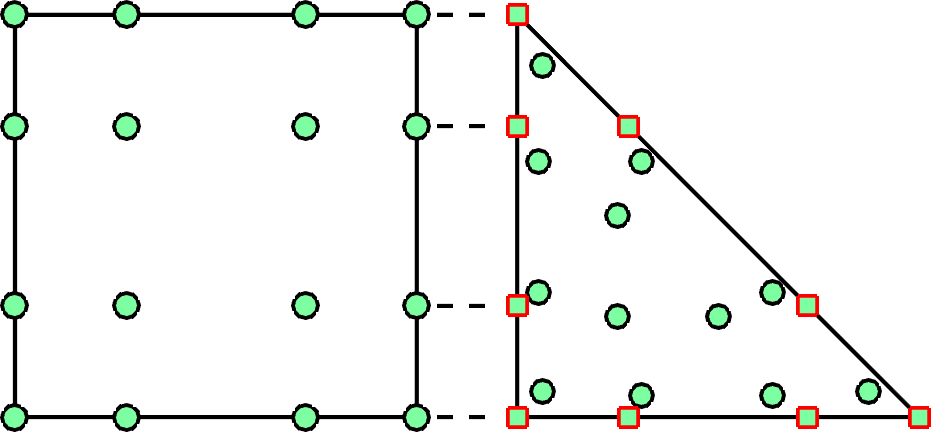
\includegraphics[width=.45\textwidth]{figs/hybrid2D.png}}
\hspace{1em}
\subfloat[No SBP (quad.\ under-integrated)]{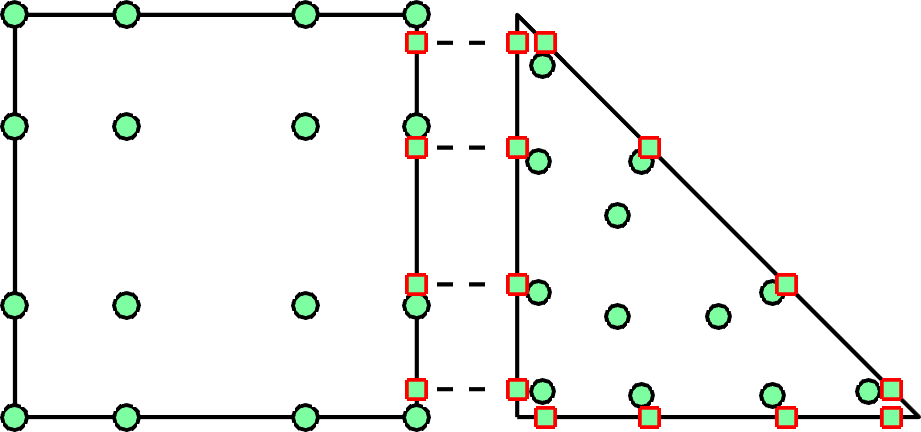
\includegraphics[width=.45\textwidth]{figs/hybrid2D_GQ.png}}
\end{figure}
\vspace{.5em}
\begin{itemize}
\item GSBP property lost if surface quadrature insufficiently accurate.
\item Skew-symmetric formulation remains entropy stable under ``weak'' GSBP property, relaxed requirements on quadrature accuracy.
\end{itemize}
%\[
%\bm{M}\td{{\bm{u}}}{t} + \sum_{i=1}^d\LRs{\begin{array}{c}
%\bm{V}_q \\ \bm{V}_f\end{array}}^T \LRp{\LRp{\bm{Q}^i_N-\LRp{\bm{Q}^i_N}^T} \circ \bm{F}^i_S}\bm{1} + \bm{V}_f^T\bm{B}_i \bm{f}^i_S(\tilde{\bm{u}}^+,\tilde{\bm{u}}) = 0.
%\]
\let\thefootnote\relax\footnotetext{\tiny Chan (2019). \textit{Skew-symmetric entropy stable modal discontinuous Galerkin formulations}.}
}

\frame{
\frametitle{Numerical results: mixed triangle-quadrilateral meshes}
\setcounter{subfigure}{0}
\begin{figure}
\centering
\subfloat[Coarse hybrid mesh]{\raisebox{2.75em}{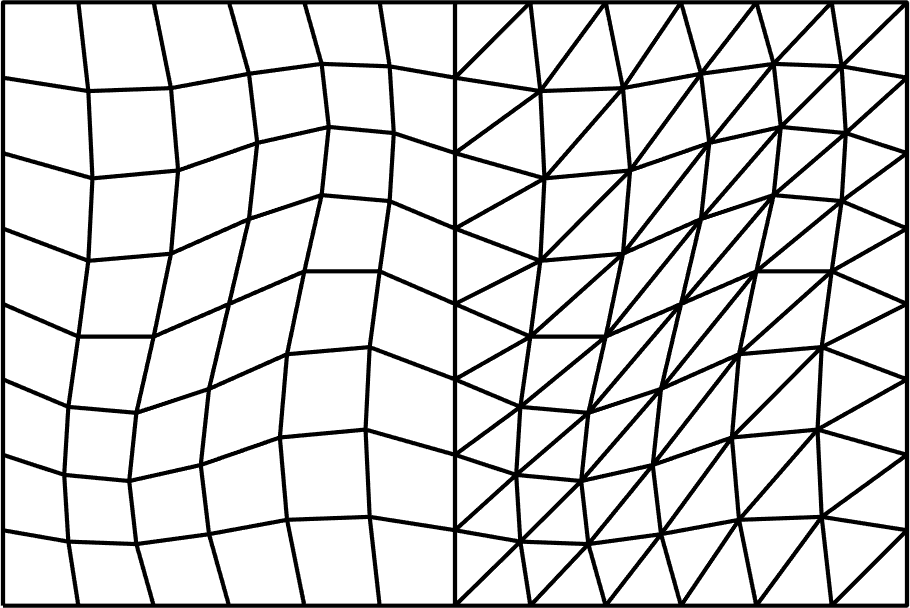
\includegraphics[width=.45\textwidth]{figs/hybrid_mesh.png}}}
\hspace{.25em}
\subfloat[$L^2$ errors for $N = 1,2,3,4$]{
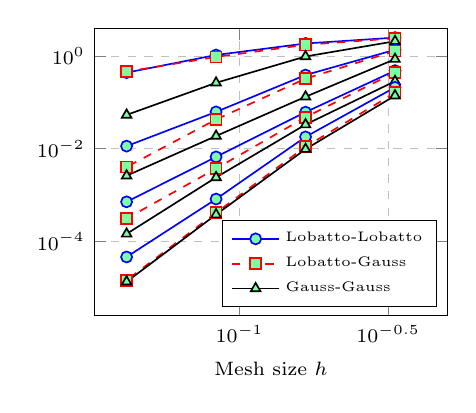
\begin{tikzpicture}
\begin{loglogaxis}[
    width=.5\textwidth,
    xlabel={Mesh size $h$},
%    ylabel={$L^2$ errors}, 
    xmax=.5,
    ymin=2.5e-6, ymax=4,
    legend pos=south east, legend cell align=left, legend style={font=\tiny},	
    xmajorgrids=true, ymajorgrids=true, grid style=dashed,
    legend entries={Lobatto-Lobatto, Lobatto-Gauss, Gauss-Gauss} 
]
\pgfplotsset{
cycle list={{blue, mark=*}, {red, dashed ,mark=square*},{black ,mark=triangle*}}
}
\addplot+[semithick, mark options={solid, fill=markercolor}]
coordinates{(0.333333,2.50656)(0.166667,1.874)(0.0833333,1.05647)(0.0416667,0.438926)};
\addplot+[semithick, mark options={solid, fill=markercolor}]
coordinates{(0.333333,2.42633)(0.166667,1.75142)(0.0833333,0.958902)(0.0416667,0.462137)};
\addplot+[semithick, mark options={solid, fill=markercolor}]
coordinates{(0.333333,2.09363)(0.166667,0.981664)(0.0833333,0.264928)(0.0416667,0.0536376)};
\addplot+[semithick, mark options={solid, fill=markercolor}]
coordinates{(0.333333,1.36947)(0.166667,0.390076)(0.0833333,0.0623387)(0.0416667,0.011361)};
\addplot+[semithick, mark options={solid, fill=markercolor}]
coordinates{(0.333333,1.28187)(0.166667,0.326338)(0.0833333,0.0427717)(0.0416667,0.00402484)};
\addplot+[semithick, mark options={solid, fill=markercolor}]
coordinates{(0.333333,0.859449)(0.166667,0.132239)(0.0833333,0.0187852)(0.0416667,0.0026063)};
\addplot+[semithick, mark options={solid, fill=markercolor}]
coordinates{(0.333333,0.48545)(0.166667,0.0615538)(0.0833333,0.00665061)(0.0416667,0.000711264)};
\addplot+[semithick, mark options={solid, fill=markercolor}]
coordinates{(0.333333,0.446407)(0.166667,0.0477486)(0.0833333,0.00372164)(0.0416667,0.000309705)};
\addplot+[semithick, mark options={solid, fill=markercolor}]
coordinates{(0.333333,0.286258)(0.166667,0.0331728)(0.0833333,0.00239593)(0.0416667,0.000144346)};
\addplot+[semithick, mark options={solid, fill=markercolor}]
coordinates{(0.333333,0.211329)(0.166667,0.0179798)(0.0833333,0.000816429)(0.0416667, 4.583068530777824e-05)};
\addplot+[semithick, mark options={solid, fill=markercolor}]
coordinates{(0.333333,0.160937)(0.166667,0.0110045)(0.0833333,0.00041413)(0.0416667, 1.438708299584088e-05)};
\addplot+[semithick, mark options={solid, fill=markercolor}]
coordinates{(0.333333,0.13975)(0.166667,0.00977304)(0.0833333,0.00037731)(0.0416667, 1.337566281886131e-05)};
%\node at (axis cs:.55,2.5) {$N = 1$};
%\node at (axis cs:.55,.82) {$N = 2$};
%\node at (axis cs:.55,.25) {$N = 3$};
%\node at (axis cs:.55,.08) {$N = 4$};
\end{loglogaxis}
\end{tikzpicture}
}
\end{figure}

\begin{center}
The skew-symmetric formulation guarantees entropy stability for all combinations of Lobatto and Gauss volume and surface quadratures.
\end{center}
}


\frame{
\frametitle{Non-conforming interfaces}
\setcounter{subfigure}{0}
%\begin{overlayarea}{\textwidth}{\textheight}

\begin{figure}
\centering
\subfloat[Conforming surface quadrature nodes]{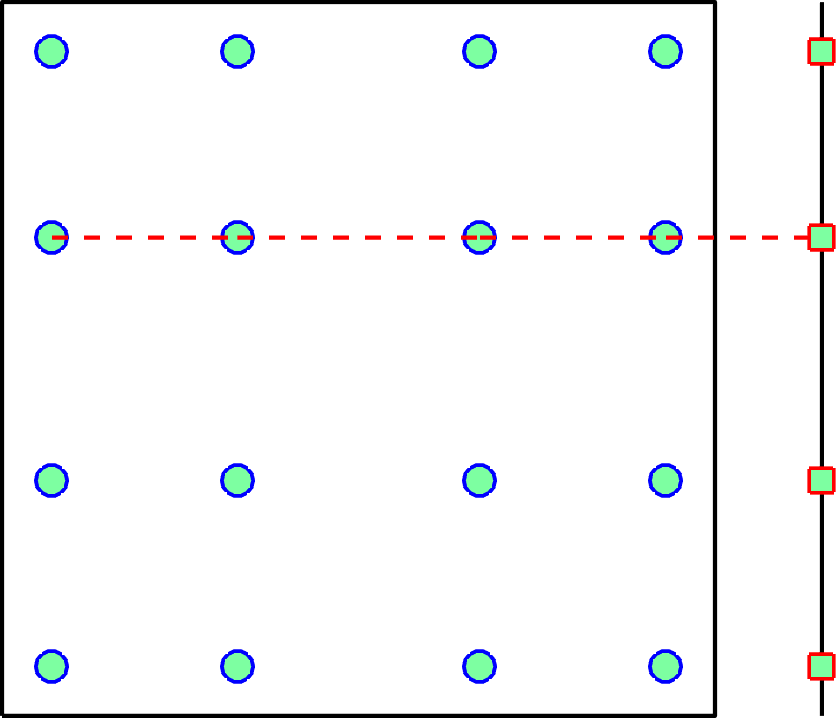
\includegraphics[height=.375\textheight]{figs/aligned.png}}
\hspace{5em}
\subfloat[Non-conforming surface nodes]{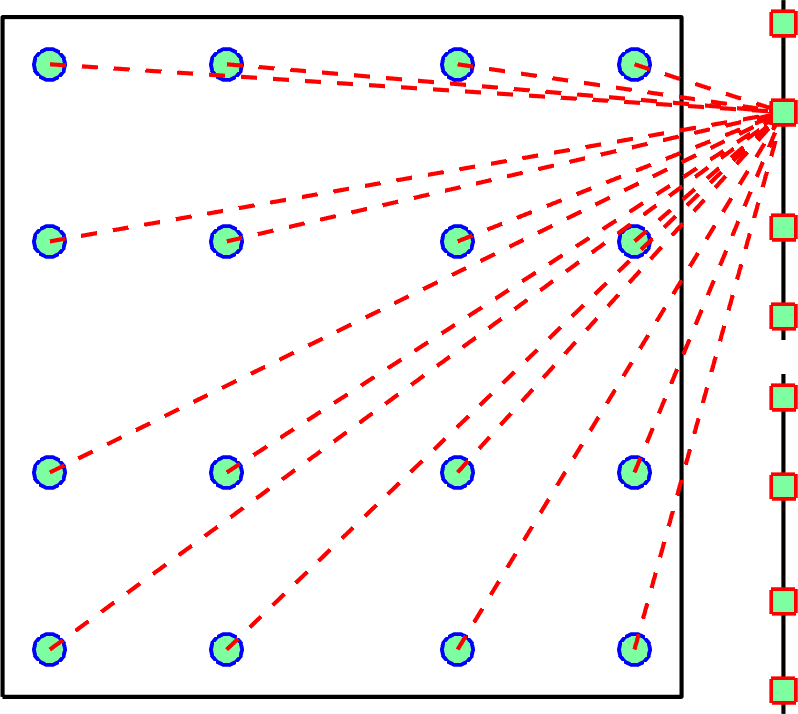
\includegraphics[height=.375\textheight]{figs/nonaligned.png}}
\end{figure}

\begin{itemize}
\item<1-> Volume/surface nodes interact through $\bm{f}_S(\bm{u}_i,\bm{u}_j)$ and \note{interpolation}.
\vspace{.25em}
\item<1-> Fix: weakly couple conforming+non-conforming faces using a mortar.
\end{itemize}
}

%\frame{
%\frametitle{Mortar implementation}
%
%\begin{figure}
%\centering
%\subfloat[Mortar operators]{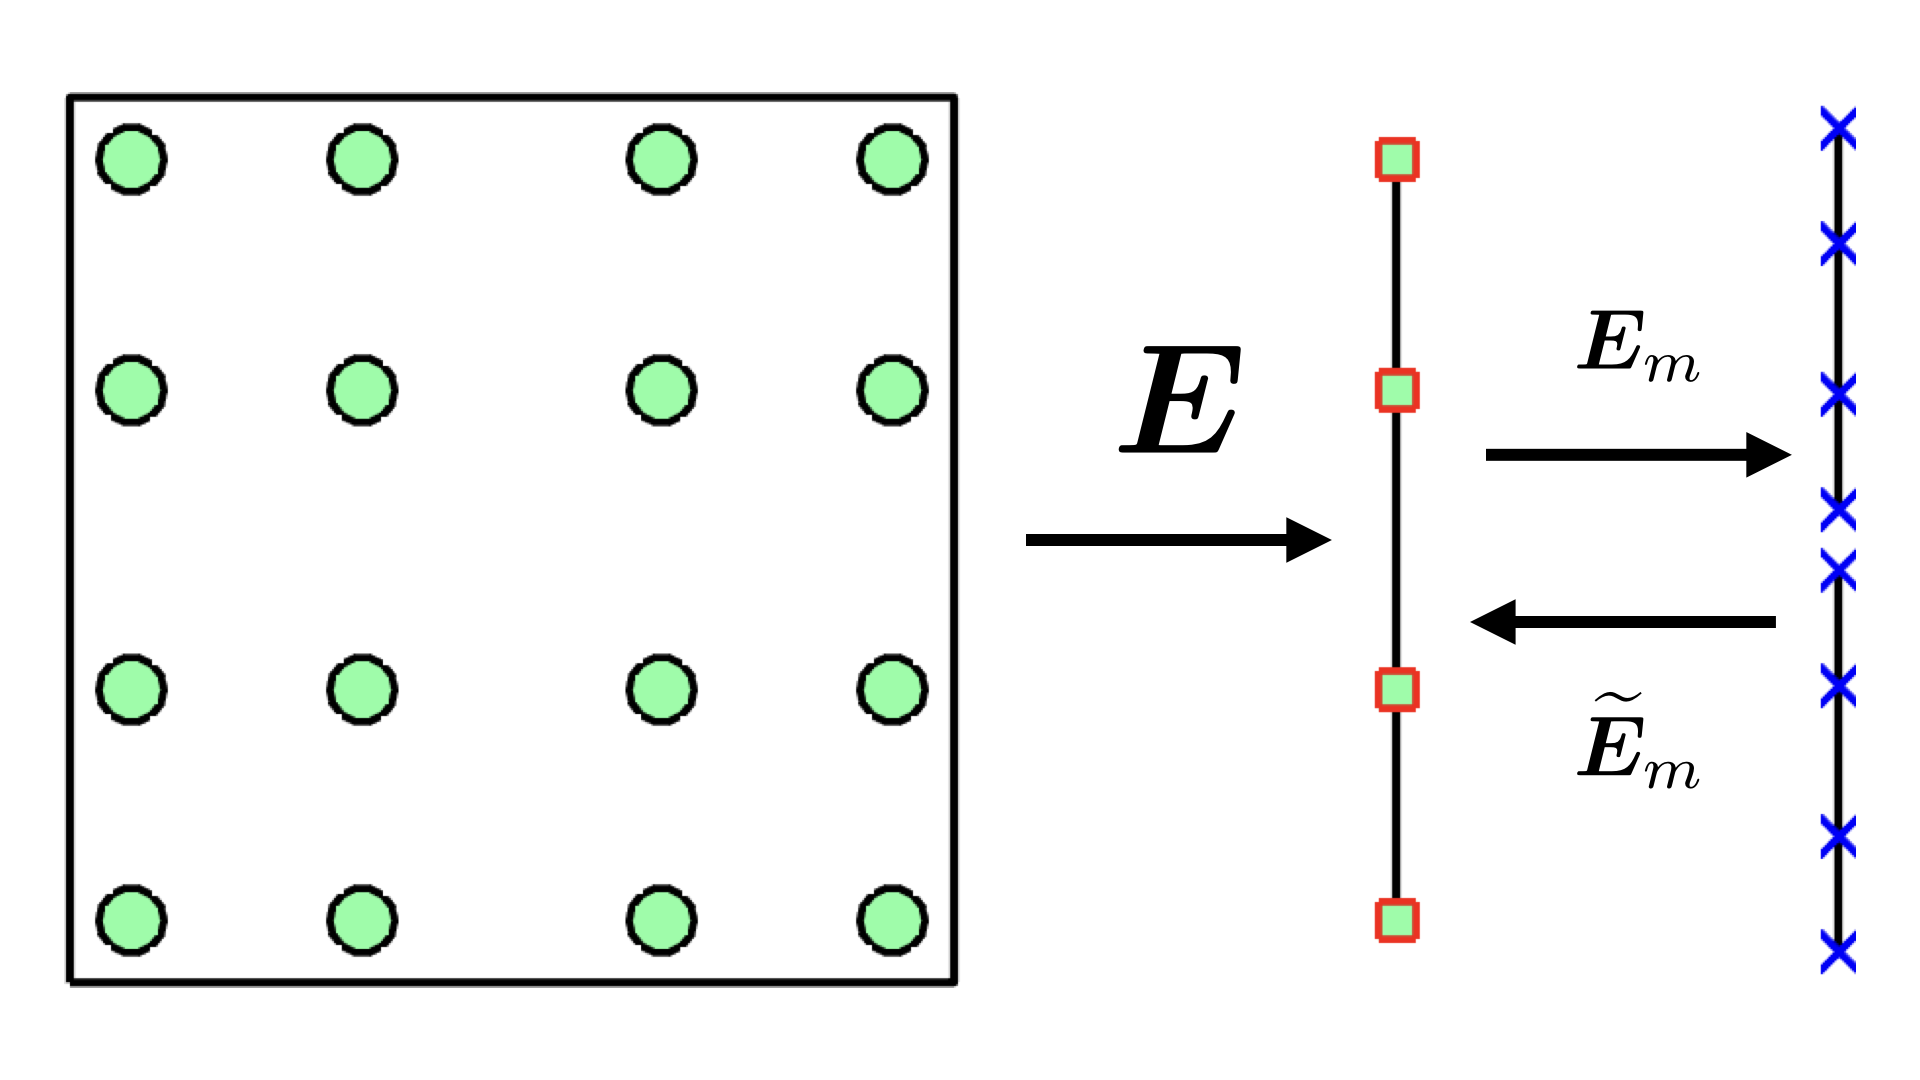
\includegraphics[width=.425\textwidth]{figs/mortar.png}}
%\hspace{1.75em}
%\subfloat[Mortar coupling]{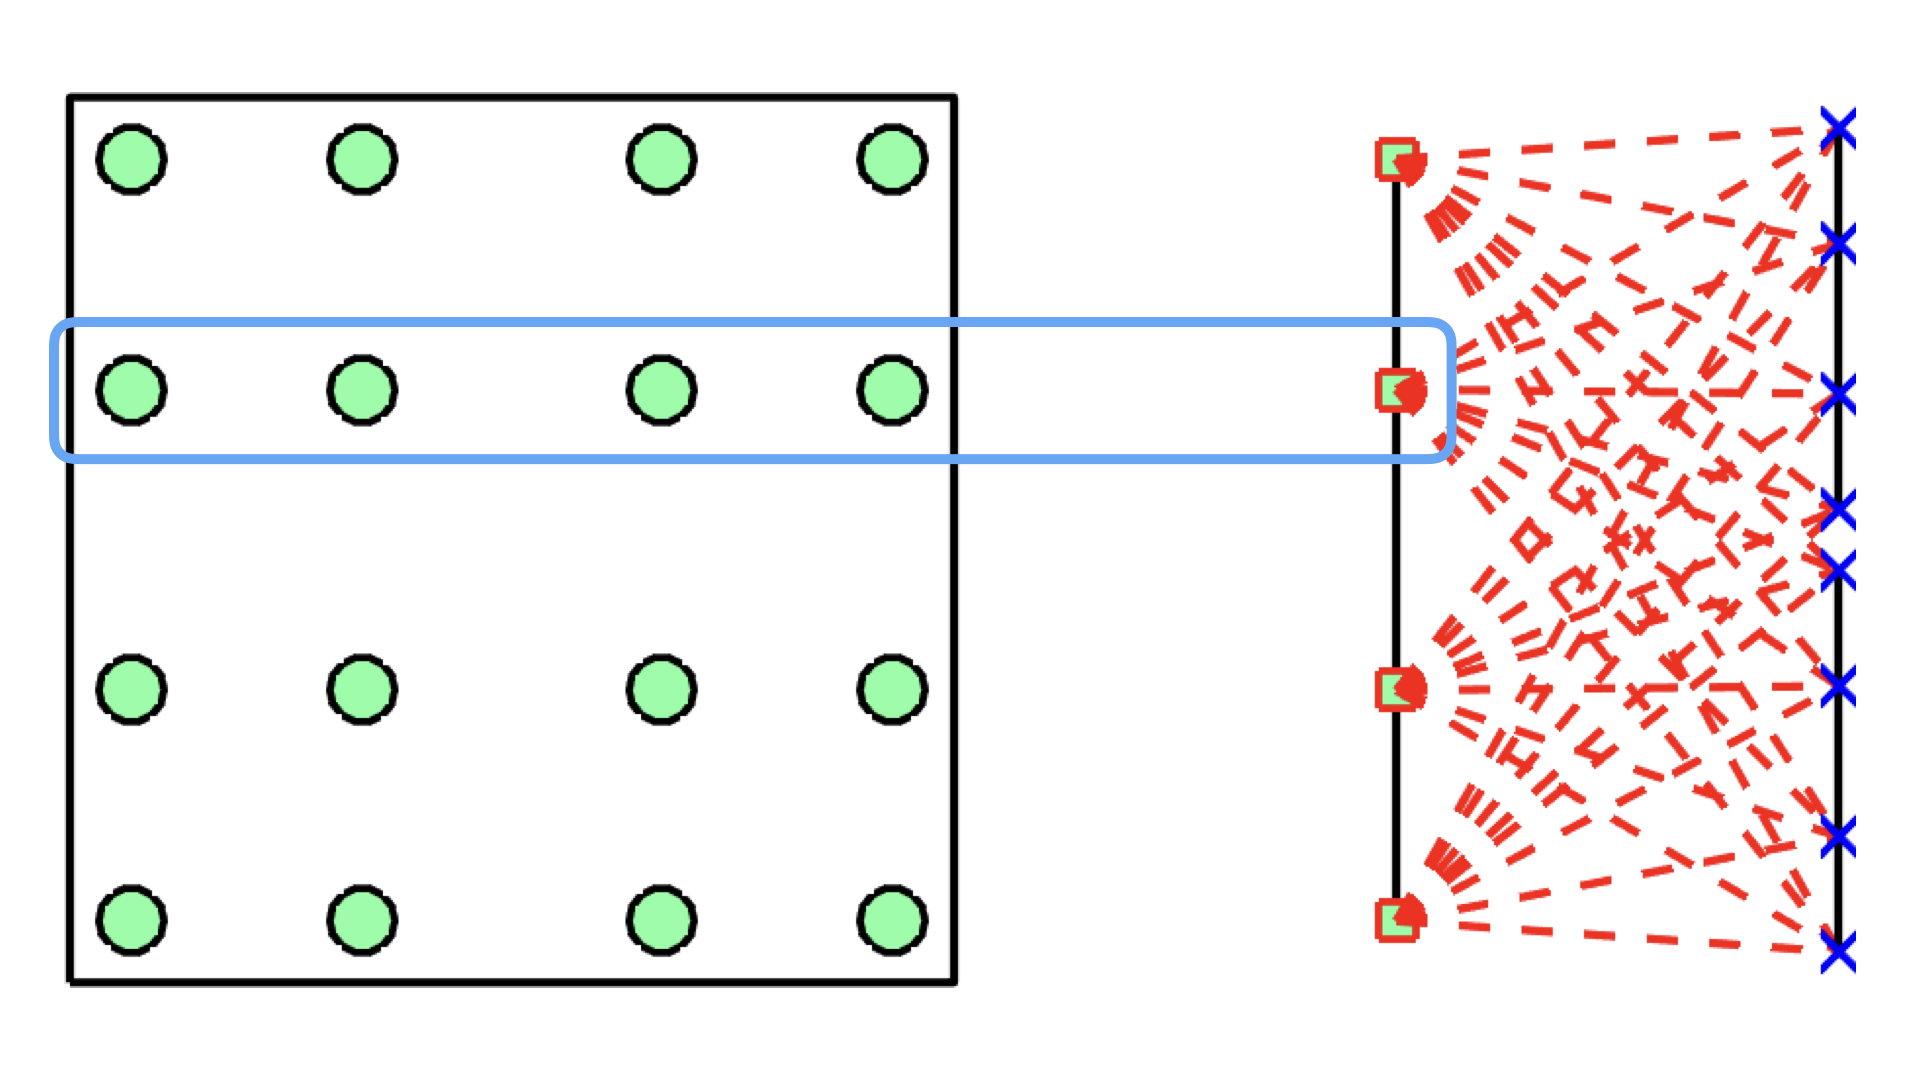
\includegraphics[width=.425\textwidth]{figs/mortar_coupling.png}}
%\end{figure}
%\begin{align*}
%\bm{M}\td{\bm{u}}{t} &+ \sum_{i=1}^d
%\begin{bmatrix} \bm{I} \\ \bm{E} \end{bmatrix}^T
%\LRp{\begin{bmatrix}
%\bm{Q}_i-\bm{Q}_i^T & \bm{E}^T\bm{B}_i\\
%-\bm{B}_i\bm{E} & \\
%\end{bmatrix} \circ \bm{F}_S}\bm{1} + \bm{E}^T\bm{B}_i \tilde{\bm{f}}^*_i = 0\\
%\tilde{\bm{f}}^*_i &= \tilde{\bm{E}}_m\bm{f}^*_i + \LRp{\tilde{\bm{E}}_m\circ \bm{F}_S^{sm}}\bm{1} - \tilde{\bm{E}}_m \LRp{ \bm{E}_m \circ \bm{F}_S^{ms}}\bm{1} 
%\end{align*}
%
%\begin{center}
%Can reformulate as an entropy stable correction to the numerical flux.  
%\end{center}
%
%}

\frame{
\frametitle{Numerical results: non-conforming meshes}

\begin{figure}
\centering
\subfloat[Coarse non-conforming mesh]{\raisebox{3em}{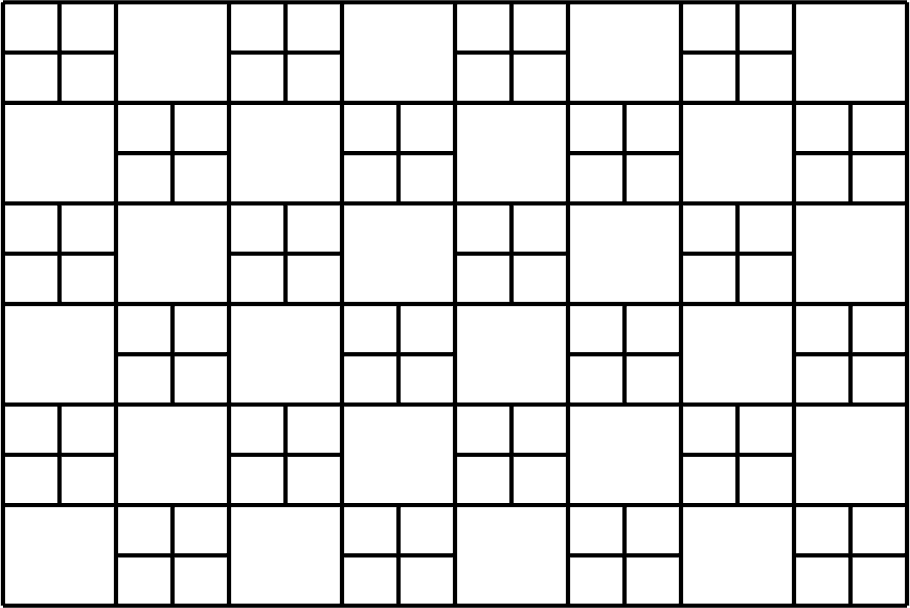
\includegraphics[width=.425\textwidth]{figs/noncon_mesh.png}}}
\hspace{.25em}
\subfloat[Sub-optimal rates if under-integrated]{
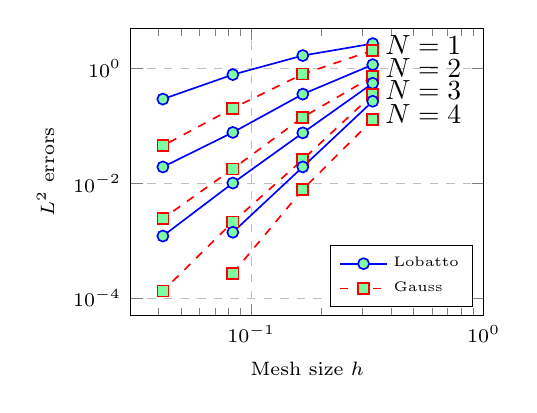
\begin{tikzpicture}
\begin{loglogaxis}[
    width=.5\textwidth,
    xlabel={Mesh size $h$},
    ylabel={$L^2$ errors}, 
    xmax=1,
    ymin=5e-5, ymax=5,
    legend pos=south east, legend cell align=left, legend style={font=\tiny},	
    xmajorgrids=true, ymajorgrids=true, grid style=dashed,
    legend entries={Lobatto, Gauss}
]
\pgfplotsset{
cycle list={{blue, mark=*}, {red, dashed ,mark=square*}}
}
\addplot+[semithick, mark options={solid, fill=markercolor}]
coordinates{(0.333333,2.6993)(0.166667,1.6718)(0.0833333,0.7792)(0.0416667,0.29211)};
\addplot+[semithick, mark options={solid, fill=markercolor}]
coordinates{(0.333333,2.0534)(0.166667,0.7966)(0.0833333,0.2022)(0.0416667,0.0449413)};

\addplot+[semithick, mark options={solid, fill=markercolor}]
coordinates{(0.333333,1.1609)(0.166667,0.3562)(0.0833333,0.0768)(0.0416667,0.0192197)};
\addplot+[semithick, mark options={solid, fill=markercolor}]
coordinates{(0.333333,0.7191)(0.166667,0.141)(0.0833333,0.0178)(0.0416667,0.00243087)};

\addplot+[semithick, mark options={solid, fill=markercolor}]
coordinates{(0.333333,0.551145)(0.166667,0.0754237)(0.0833333,0.0100808)(0.0416667,0.00120633)};
\addplot+[semithick, mark options={solid, fill=markercolor}]
coordinates{(0.333333,0.352706)(0.166667,0.0258415)(0.0833333,0.00211953)(0.0416667,0.000132969)};

\addplot+[semithick, mark options={solid, fill=markercolor}]
coordinates{(0.333333,0.267668)(0.166667,0.0192603)(0.0833333,0.00140341)};
\addplot+[semithick, mark options={solid, fill=markercolor}]
coordinates{(0.333333,0.128217)(0.166667,0.00779943)(0.0833333,0.000270803)};

\node at (axis cs:.55,2.5) {$N = 1$};
\node at (axis cs:.55,1.0) {$N = 2$};
\node at (axis cs:.55,.42) {$N = 3$};
\node at (axis cs:.55,.16) {$N = 4$};
\end{loglogaxis}
\end{tikzpicture}
}
\end{figure}

\begin{center}
The skew-symmetric formulation guarantees entropy stability for both Lobatto and Gauss quadratures, but Gauss is more accurate.
\end{center}

%\let\thefootnote\relax\footnotetext{\tiny Chan (2019). \textit{Skew-symmetric entropy stable modal discontinuous Galerkin formulations}.}
}

%\frame{
%\frametitle{Meshes with non-conforming interfaces}
%
%%\begin{overlayarea}{\textwidth}{\textheight}
%
%\only<1>{
%\vspace{-.5em}
%\begin{figure}
%\centering
%\subfloat[Conforming surface quadrature nodes]{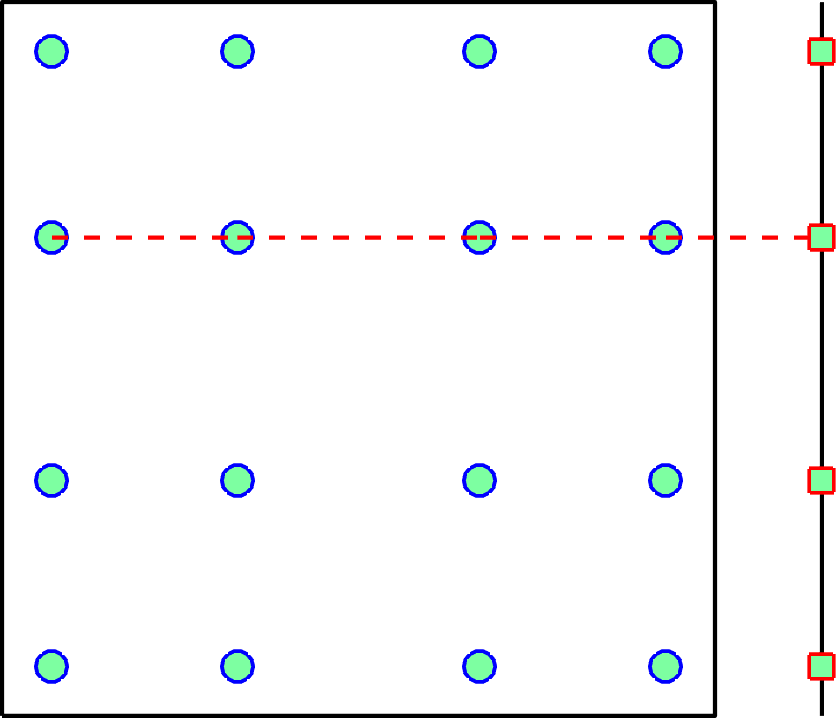
\includegraphics[height=.32\textheight]{figs/aligned.png}}
%\hspace{5em}
%\subfloat[Non-conforming surface nodes]{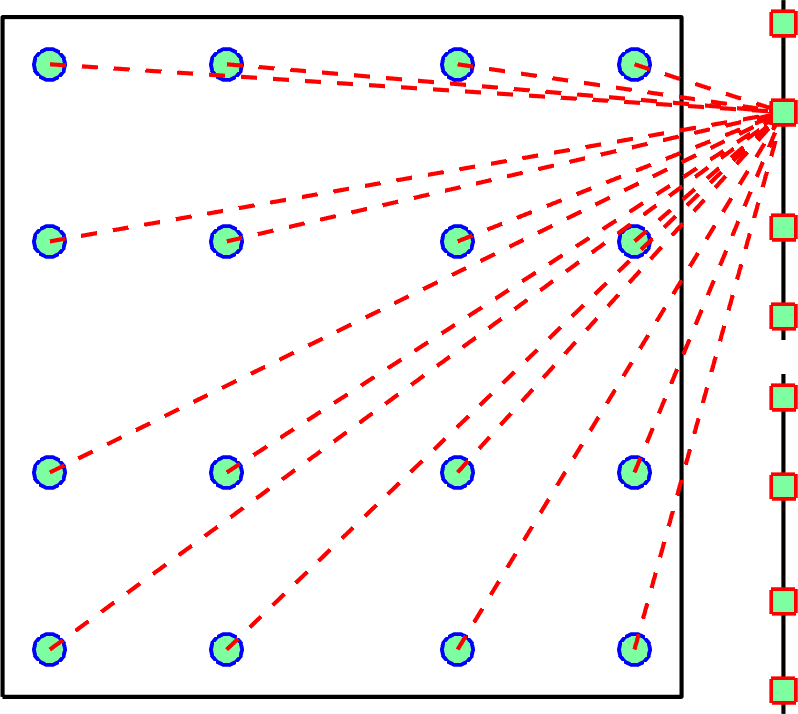
\includegraphics[height=.32\textheight]{figs/nonaligned.png}}
%\end{figure}
%}% only
%
%\only<2-3>{
%\begin{columns}
%
%\column{0.45\textwidth}
%\begin{figure}
%\centering
%\begin{overlayarea}{\textwidth}{.375\textheight}
%\only<2>{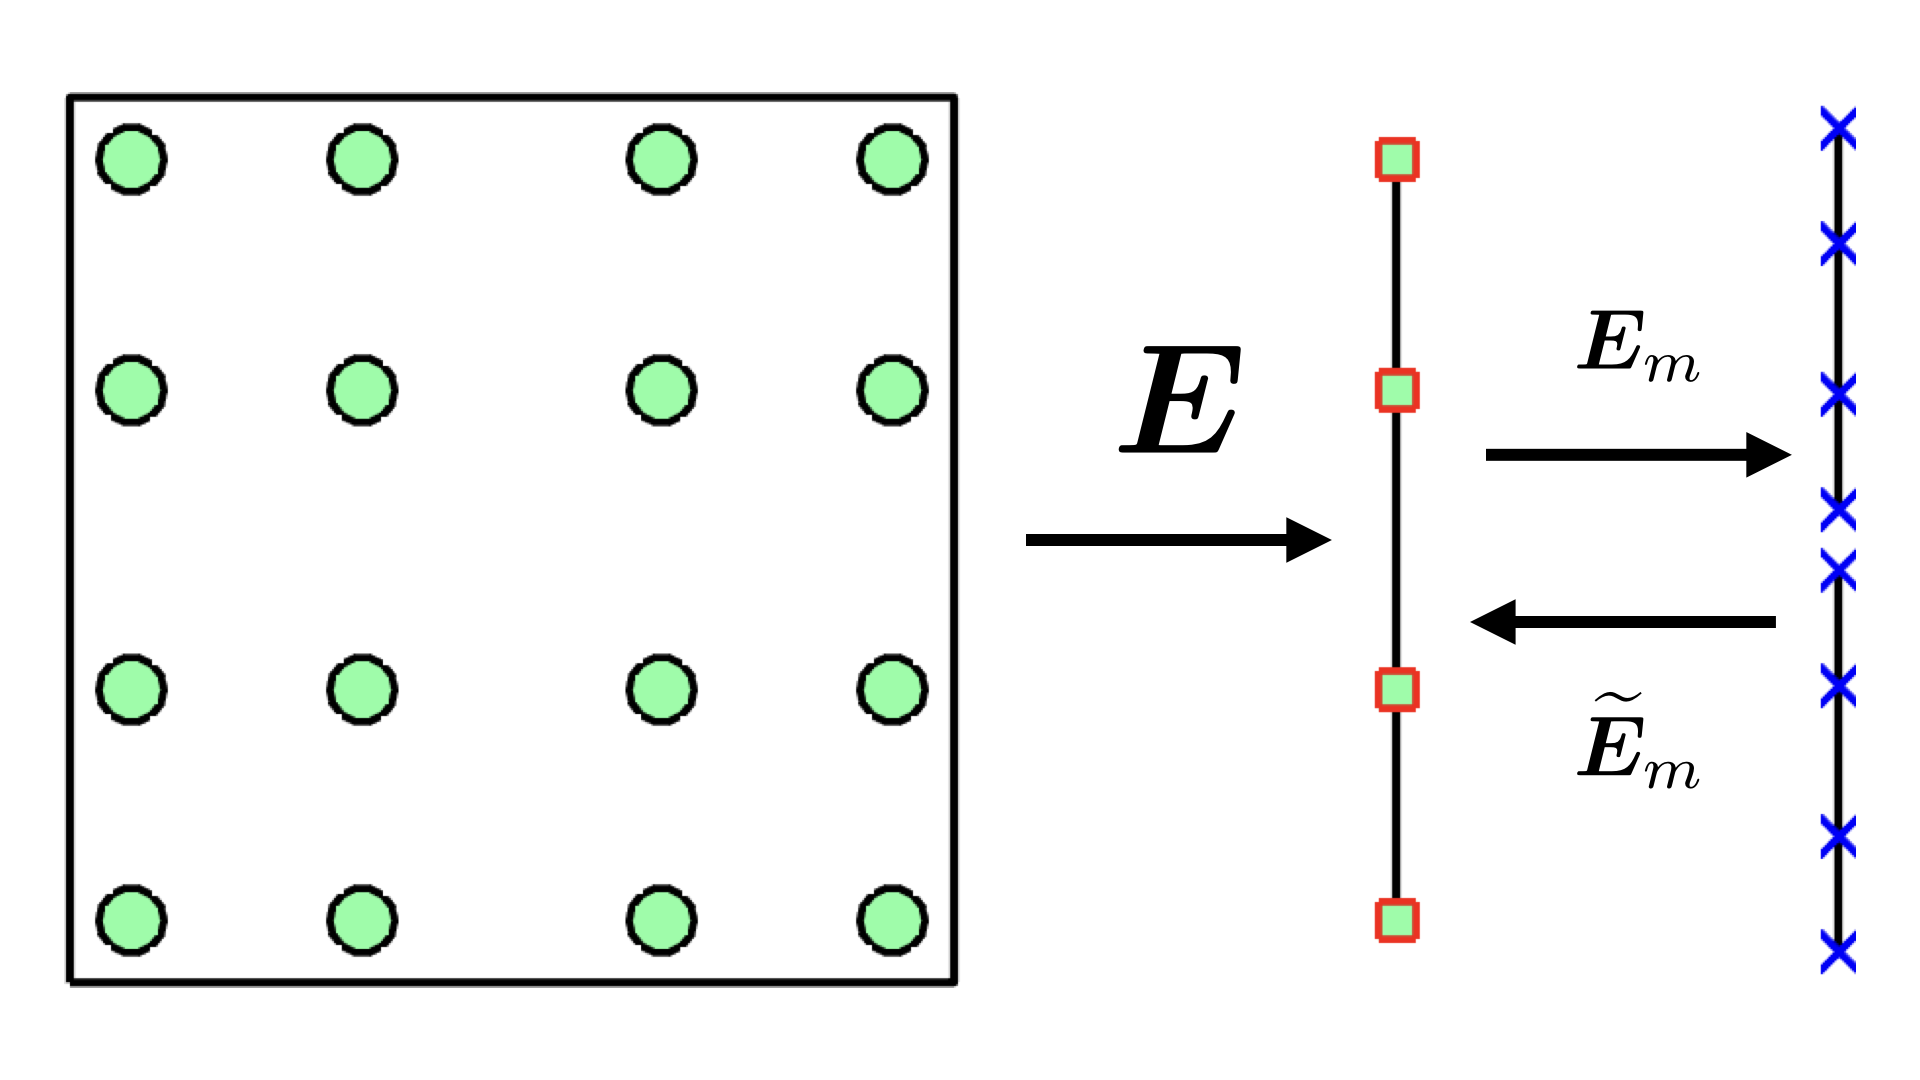
\includegraphics[width=\textwidth]{figs/mortar.png}}
%\only<3>{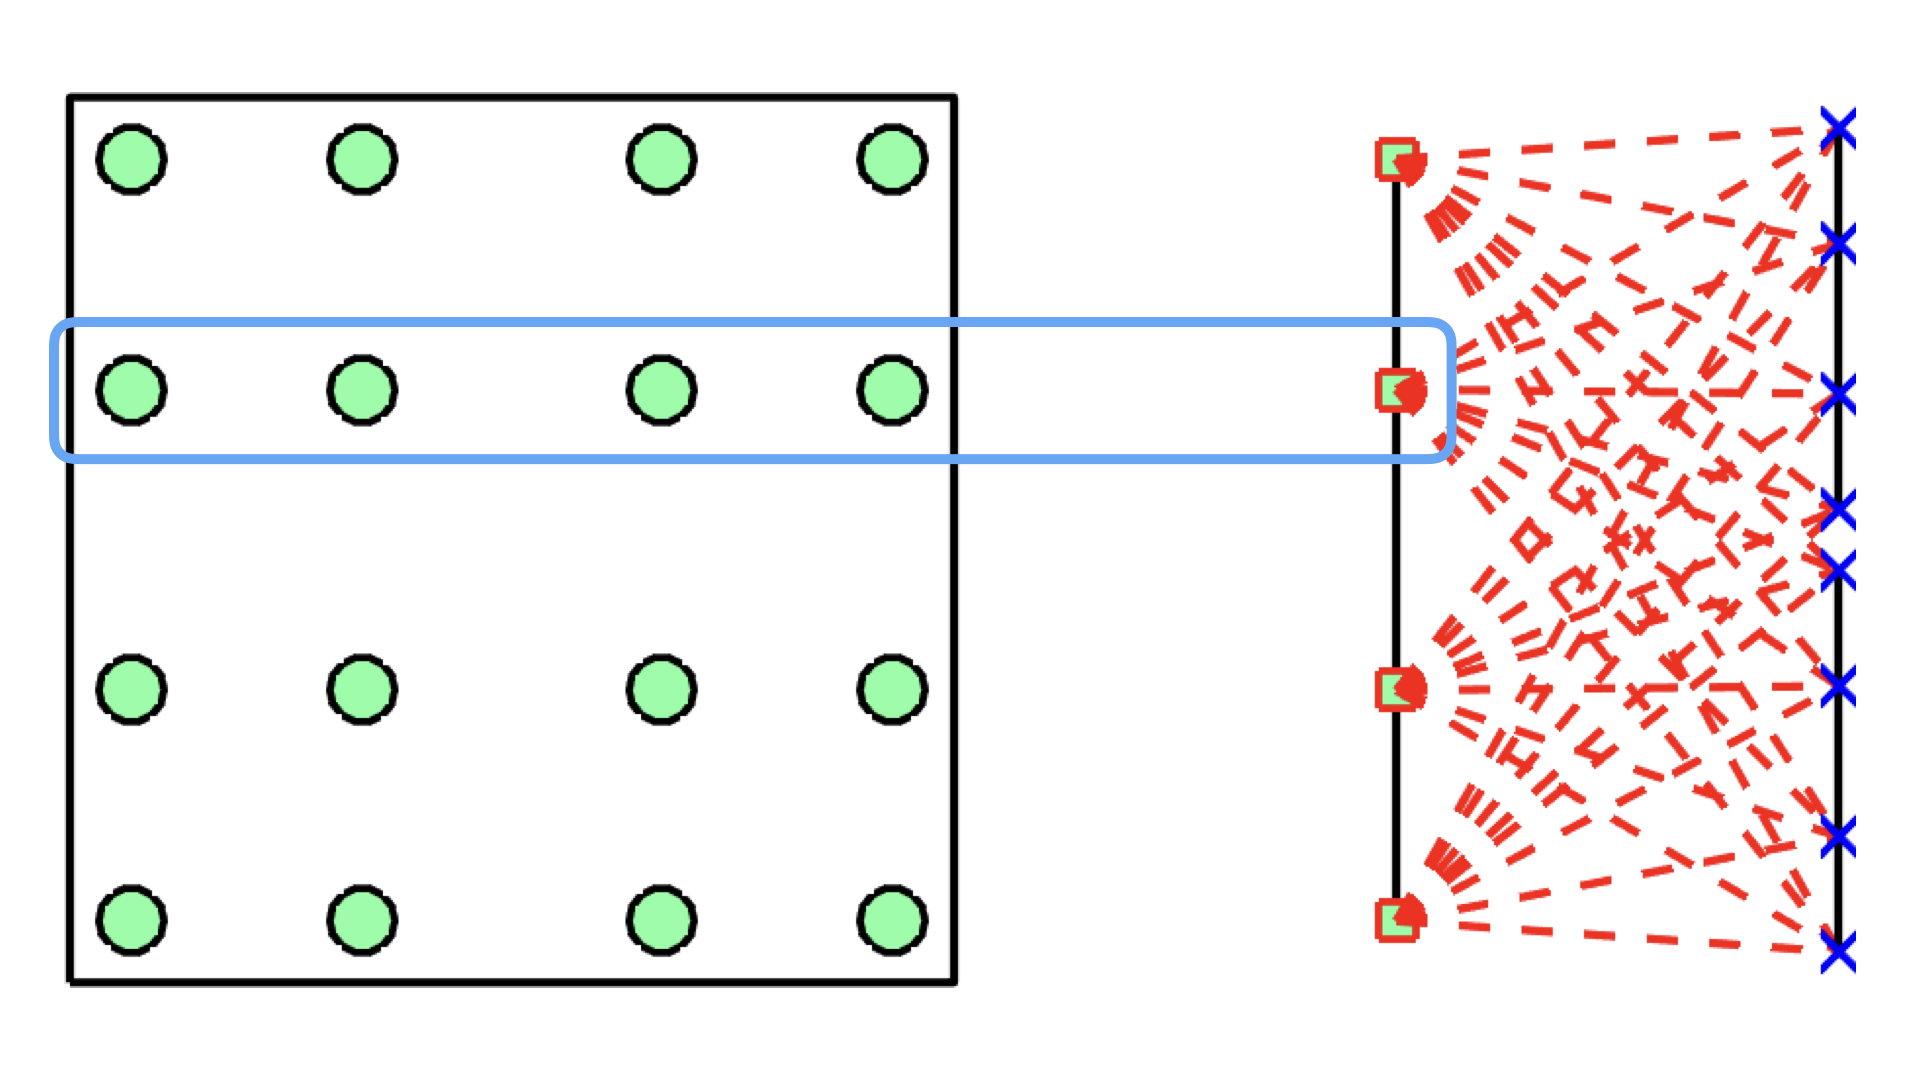
\includegraphics[width=\textwidth]{figs/mortar_coupling.png}}
%\end{overlayarea}
%\end{figure}
%
%\column{0.475\textwidth}
%%\setlength\arraycolsep{2em}
%\begin{equation*}
%%\bm{M}\td{\bm{u}_N}{t} + \begin{bmatrix} \bm{V}_q \\ \bm{V}_f \\ \bm{V}_m \end{bmatrix}^T
%%\LRp{
%\underbrace{\begin{bmatrix}
%\bm{Q}_i-\bm{Q}_i^T & \bm{E}^T\bm{B}_i &\\
%-\bm{B}_i\bm{E} &  & \bm{B}_i\tilde{\bm{E}}_m \\
%& -\tilde{\bm{B}}_i{\bm{E}}_m & 
%\end{bmatrix}}_{\text{modified skew operator } \bm{Q}^i_N- \LRp{\bm{Q}^i_N}^T}
%%\circ \bm{F}_S}\bm{1} + \bm{V}_m^T\tilde{\bm{B}}_i\bm{f}_i^* = 0.  
%%\label{eq:mortar}
%\end{equation*}
%
%\end{columns}
%\vspace{.5em}
%}% only
%
%
%\begin{itemize}
%\item<1-> Volume/surface nodes interact through $\bm{f}_S(\bm{u}_i,\bm{u}_j)$ and \note{interpolation}.
%\vspace{.25em}
%\item<2-> Weakly couple volume nodes to non-conforming surface nodes by adding conforming ``mortar'' (via additional blocks in $\bm{Q}_N$).
%\vspace{.25em}
%\item<2-> Can reformulate as an entropy stable correction to standard mortar.  
%\end{itemize}
%
%%\end{overlayarea}
%}
%
%\frame{
%\frametitle{Numerical results: non-conforming meshes}
%
%\begin{figure}
%\centering
%\subfloat[Coarse non-conforming mesh]{\raisebox{3em}{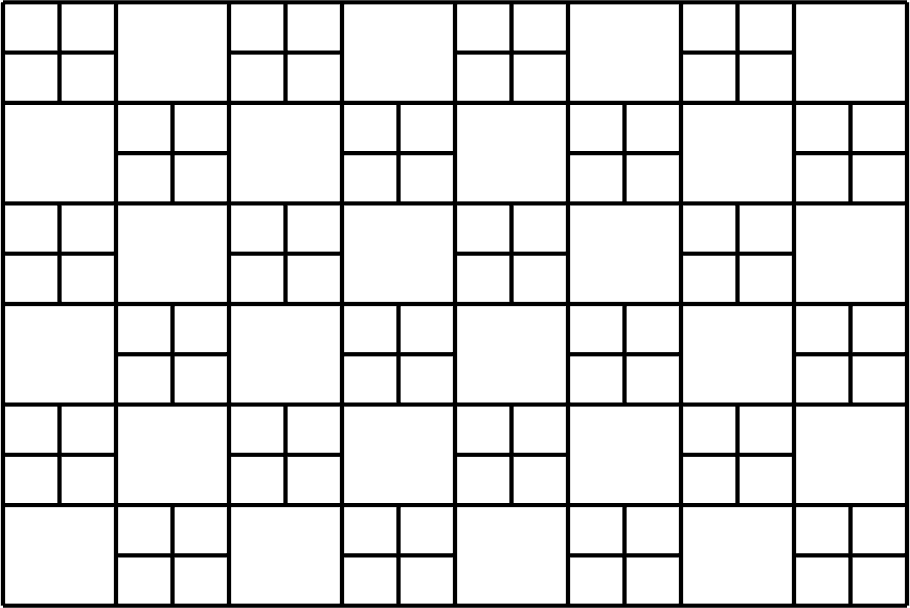
\includegraphics[width=.425\textwidth]{figs/noncon_mesh.png}}}
%\hspace{.25em}
%\subfloat[Sub-optimal rates if under-integrated]{
%\begin{tikzpicture}
%\begin{loglogaxis}[
%    width=.5\textwidth,
%    xlabel={Mesh size $h$},
%    ylabel={$L^2$ errors}, 
%    xmax=1,
%    ymin=5e-5, ymax=5,
%    legend pos=south east, legend cell align=left, legend style={font=\tiny},	
%    xmajorgrids=true, ymajorgrids=true, grid style=dashed,
%    legend entries={Lobatto, Gauss}
%]
%\pgfplotsset{
%cycle list={{blue, mark=*}, {red, dashed ,mark=square*}}
%}
%\addplot+[semithick, mark options={solid, fill=markercolor}]
%coordinates{(0.333333,2.6993)(0.166667,1.6718)(0.0833333,0.7792)(0.0416667,0.29211)};
%\addplot+[semithick, mark options={solid, fill=markercolor}]
%coordinates{(0.333333,2.0534)(0.166667,0.7966)(0.0833333,0.2022)(0.0416667,0.0449413)};
%
%\addplot+[semithick, mark options={solid, fill=markercolor}]
%coordinates{(0.333333,1.1609)(0.166667,0.3562)(0.0833333,0.0768)(0.0416667,0.0192197)};
%\addplot+[semithick, mark options={solid, fill=markercolor}]
%coordinates{(0.333333,0.7191)(0.166667,0.141)(0.0833333,0.0178)(0.0416667,0.00243087)};
%
%\addplot+[semithick, mark options={solid, fill=markercolor}]
%coordinates{(0.333333,0.551145)(0.166667,0.0754237)(0.0833333,0.0100808)(0.0416667,0.00120633)};
%\addplot+[semithick, mark options={solid, fill=markercolor}]
%coordinates{(0.333333,0.352706)(0.166667,0.0258415)(0.0833333,0.00211953)(0.0416667,0.000132969)};
%
%\addplot+[semithick, mark options={solid, fill=markercolor}]
%coordinates{(0.333333,0.267668)(0.166667,0.0192603)(0.0833333,0.00140341)};
%\addplot+[semithick, mark options={solid, fill=markercolor}]
%coordinates{(0.333333,0.128217)(0.166667,0.00779943)(0.0833333,0.000270803)};
%
%\node at (axis cs:.55,2.5) {$N = 1$};
%\node at (axis cs:.55,1.0) {$N = 2$};
%\node at (axis cs:.55,.42) {$N = 3$};
%\node at (axis cs:.55,.16) {$N = 4$};
%\end{loglogaxis}
%\end{tikzpicture}
%}
%\end{figure}
%
%\begin{center}
%The skew-symmetric formulation guarantees entropy stability for both Lobatto and Gauss quadratures, but Gauss is more accurate.
%\end{center}
%}



%% =================================================

\frame{
\frametitle{Summary and future work}

\begin{itemize}
\item Entropy stable high order ``modal'' DG: flexibility in choosing basis and quadrature, improved accuracy on curved meshes.
\vspace{.25em}
\item Current work: ROMs, strong shocks, positivity preservation.  
\vspace{.25em}
%\item Current work: hybrid and non-conforming meshes, multi-GPU.
%\vspace{.25em}
\item This work is supported by DMS-1719818 and DMS-1712639. 
\end{itemize}
\vspace{.25em}
\begin{center}
Thank you!  Questions?
\vspace{.25em}

{
\includegraphics[width=.15\textwidth]{figs/nsf.jpg}}
\end{center}

\let\thefootnote\relax\footnotetext{\tiny Chan (2019). \textit{Skew-symmetric entropy stable modal discontinuous Galerkin formulations}.}
\let\thefootnote\relax\footnotetext{\tiny Chan, Del Rey Fernandez, Carpenter (2018). \textit{Efficient entropy stable Gauss collocation methods}.}
\let\thefootnote\relax\footnotetext{\tiny Chan, Wilcox (2018). \textit{On discretely entropy stable weight-adjusted DG methods: curvilinear meshes}.}
\let\thefootnote\relax\footnotetext{\tiny Chan (2018). \textit{On discretely entropy conservative and entropy stable discontinuous Galerkin methods.}}
}

%% =================================================


\begin{frame}[noframenumbering]
\frametitle{Additional slides }
\end{frame}

\frame[noframenumbering]{
\frametitle{Decoupled SBP operators add boundary corrections}
\vspace{-.5em}
\begin{figure}
\centering
\subfloat[Derivative approximations]{
\label{subfig:dsbp1}
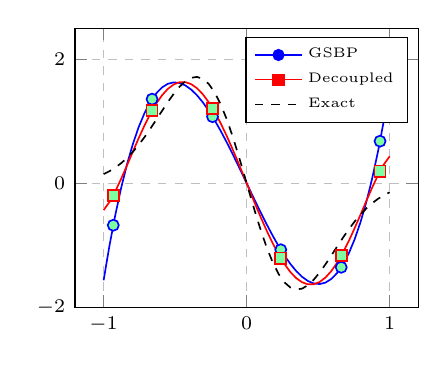
\begin{tikzpicture}
\begin{axis}[
    width=.49\textwidth,
%    xlabel={$x$ coordinate},
%    ylabel={$\pd{u}{x}$}, 
%    xmin=.0125, xmax=.75,
    ymin=-2, ymax=2.5,
    legend pos=north east, legend cell align=left, legend style={font=\tiny},	
    xmajorgrids=true, ymajorgrids=true, grid style=dashed,
    legend entries={GSBP, Decoupled, Exact}    
]
\pgfplotsset{
cycle list={{blue, only marks, mark=*}, {blue}, {red, only marks,mark=square*},{red},{black,dashed}}
}
\addlegendimage{blue, mark=*}
\addlegendimage{red, mark=square*}
\addlegendimage{black, dashed}

\addplot+[semithick, mark options={solid, fill=markercolor}]
coordinates{(-0.93247,-0.677965)(-0.661209,1.35632)(-0.238619,1.07263)(0.238619,-1.07263)(0.661209,-1.35632)(0.93247,0.677965)};

\addplot+[semithick, mark options={solid, fill=markercolor}]
coordinates{(-1,-1.56577)(-0.959184,-1.00891)(-0.918367,-0.51366)(-0.877551,-0.0774098)(-0.836735,0.302464)(-0.795918,0.628585)(-0.755102,0.903575)(-0.714286,1.13006)(-0.673469,1.31065)(-0.632653,1.44798)(-0.591837,1.54466)(-0.55102,1.60333)(-0.510204,1.62659)(-0.469388,1.61708)(-0.428571,1.57742)(-0.387755,1.51022)(-0.346939,1.41812)(-0.306122,1.30372)(-0.265306,1.16966)(-0.22449,1.01856)(-0.183673,0.85303)(-0.142857,0.675704)(-0.102041,0.489201)(-0.0612245,0.296143)(-0.0204082,0.0991513)(0.0204082,-0.0991513)(0.0612245,-0.296143)(0.102041,-0.489201)(0.142857,-0.675704)(0.183673,-0.85303)(0.22449,-1.01856)(0.265306,-1.16966)(0.306122,-1.30372)(0.346939,-1.41812)(0.387755,-1.51022)(0.428571,-1.57742)(0.469388,-1.61708)(0.510204,-1.62659)(0.55102,-1.60333)(0.591837,-1.54466)(0.632653,-1.44798)(0.673469,-1.31065)(0.714286,-1.13006)(0.755102,-0.903575)(0.795918,-0.628585)(0.836735,-0.302464)(0.877551,0.0774098)(0.918367,0.51366)(0.959184,1.00891)(1,1.56577)};

\addplot+[semithick, mark options={solid, fill=markercolor}]
coordinates{(-0.93247,-0.194074)(-0.661209,1.16978)(-0.238619,1.20913)(0.238619,-1.20913)(0.661209,-1.16978)(0.93247,0.194074)};

\addplot+[semithick, mark options={solid, fill=markercolor}]
coordinates{(-1,-0.434491)(-0.959184,-0.303266)(-0.918367,-0.130624)(-0.877551,0.0698403)(-0.836735,0.286078)(-0.795918,0.507515)(-0.755102,0.724981)(-0.714286,0.930644)(-0.673469,1.11794)(-0.632653,1.28151)(-0.591837,1.41712)(-0.55102,1.5216)(-0.510204,1.59278)(-0.469388,1.62942)(-0.428571,1.63111)(-0.387755,1.59825)(-0.346939,1.53198)(-0.306122,1.43404)(-0.265306,1.30681)(-0.22449,1.15314)(-0.183673,0.976347)(-0.142857,0.78012)(-0.102041,0.568459)(-0.0612245,0.345602)(-0.0204082,0.115959)(0.0204082,-0.115959)(0.0612245,-0.345602)(0.102041,-0.568459)(0.142857,-0.78012)(0.183673,-0.976347)(0.22449,-1.15314)(0.265306,-1.30681)(0.306122,-1.43404)(0.346939,-1.53198)(0.387755,-1.59825)(0.428571,-1.63111)(0.469388,-1.62942)(0.510204,-1.59278)(0.55102,-1.5216)(0.591837,-1.41712)(0.632653,-1.28151)(0.673469,-1.11794)(0.714286,-0.930644)(0.755102,-0.724981)(0.795918,-0.507515)(0.836735,-0.286078)(0.877551,-0.0698403)(0.918367,0.130624)(0.959184,0.303266)(1,0.434491)};

\addplot+[semithick, mark options={solid, fill=markercolor}]
coordinates{(-1,0.146525)(-0.959184,0.193522)(-0.918367,0.251752)(-0.877551,0.322529)(-0.836735,0.406852)(-0.795918,0.50522)(-0.755102,0.617438)(-0.714286,0.742415)(-0.673469,0.877994)(-0.632653,1.02082)(-0.591837,1.1663)(-0.55102,1.30861)(-0.510204,1.44089)(-0.469388,1.55553)(-0.428571,1.64452)(-0.387755,1.70003)(-0.346939,1.71492)(-0.306122,1.68342)(-0.265306,1.60163)(-0.22449,1.46805)(-0.183673,1.2839)(-0.142857,1.05327)(-0.102041,0.783025)(-0.0612245,0.482507)(-0.0204082,0.162994)(0.0204082,-0.162994)(0.0612245,-0.482507)(0.102041,-0.783025)(0.142857,-1.05327)(0.183673,-1.2839)(0.22449,-1.46805)(0.265306,-1.60163)(0.306122,-1.68342)(0.346939,-1.71492)(0.387755,-1.70003)(0.428571,-1.64452)(0.469388,-1.55553)(0.510204,-1.44089)(0.55102,-1.30861)(0.591837,-1.1663)(0.632653,-1.02082)(0.673469,-0.877994)(0.714286,-0.742415)(0.755102,-0.617438)(0.795918,-0.50522)(0.836735,-0.406852)(0.877551,-0.322529)(0.918367,-0.251752)(0.959184,-0.193522)(1,-0.146525)};
\end{axis}
\end{tikzpicture}
}
\subfloat[$L^2$ error w.r.t.\ degree $N$]{
\label{subfig:dsbp2}
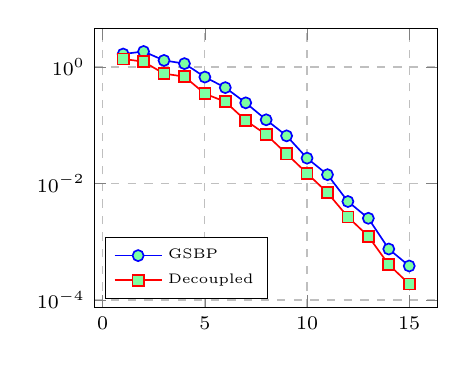
\begin{tikzpicture}
\begin{semilogyaxis}[
    width=.49\textwidth,
%    xlabel={Degree $N$},
%    ylabel={$L^2$ errors}, 
%    xmin=.0125, xmax=.75,
%    ymin=-2, ymax=2.25,
    legend pos=south west, legend cell align=left, legend style={font=\tiny},	
    xmajorgrids=true, ymajorgrids=true, grid style=dashed,
    legend entries={GSBP, Decoupled}    
]
\pgfplotsset{
cycle list={{blue, mark=*}, {red, mark=square*}}
}
%\addlegendimage{blue, mark=*}
%\addlegendimage{red, mark=square*}
%\addlegendimage{black, dashed}

\addplot+[semithick, mark options={solid, fill=markercolor}]
coordinates{(1,1.67087)(2,1.84788)(3,1.29689)(4,1.14406)(5,0.67189)(6,0.4428)(7,0.242532)(8,0.124111)(9,0.0657786)(10,0.0272413)(11,0.0141812)(12,0.00491087)(13,0.00252903)(14,0.000750851)(15,0.000383985)};

\addplot+[semithick, mark options={solid, fill=markercolor}]
coordinates{(1,1.37796)(2,1.23235)(3,0.769706)(4,0.682916)(5,0.348496)(6,0.252957)(7,0.120617)(8,0.0691975)(9,0.0323286)(10,0.0149469)(11,0.00695358)(12,0.00266351)(13,0.00124093)(14,0.000403653)(15,0.000188708)};

\end{semilogyaxis}
\end{tikzpicture}
}
%\caption{Approximations of derivatives of a Gaussian $e^{-4x^2}$ using the generalized SBP operator $\bm{D}$ and the decoupled SBP operator $\bm{Q}_N$ via (\ref{eq:qn}).  In Figure~\ref{subfig:dsbp1}, the colored circles and squares denote values at Gauss points for a degree $N = 5$ approximation.  Figure~\ref{subfig:dsbp2} shows the convergence of $L^2$ errors as $N$ increases. }
\label{fig:dsbpcorrect}
\end{figure}
\vspace{-1em}
\begin{itemize}
%\item Combine $\bm{D}^P_N$ with $L^2$ projection to approximate derivatives.
%\vspace{.25em}
%\vspace{.25em}
\item Equivalent to a variational problem for a polynomial $u(\bm{x}) \approx f\pd{g}{x}$.
\[
\int_{-1}^1u(\bm{x})v(\bm{x})  = \int_{-1}^1 {f\pd{P_Ng}{x}v} + \LRu{(g-P_Ng)\frac{\LRp{fv + P_N(fv)}}{2}}_{-1}^1.
\]
\end{itemize}
}


\frame[noframenumbering]{
\frametitle{Flux differencing: recovering split formulations}
\begin{itemize}
\item<1-> Entropy conservative flux for Burgers' equation 
\[
f_S(u_L,u_R) = \frac{1}{6}\LRp{u_L^2 + u_Lu_R + u_R^2}.
\]
\item<1-> Flux differencing: let $u_L = u(x), u_R = u(y)$
\begin{align*}
\pd{{f}({u})}{x} &\Longrightarrow \note{\LRu{2\pd{f_S\LRp{u(x),u(y)}}{x}}_{y=x}}
\end{align*}
\item<2-> Recovering the Burgers' split formulation
\begin{align*}
f_S(u(x),u(y)) &= \frac{1}{6}\LRp{u(x)^2 + u(x)u(y) + u(y)^2}\\
\LRu{2\pd{f_S\LRp{u(x),u(y)}}{x}}_{y=x} &= \frac{1}{3}\pd{u^2}{x} + \frac{1}{3}u\pd{u}{x} + \frac{1}{3}u^2\cancel{\pd{1}{x}}.
\end{align*}
\end{itemize}
}


\frame[noframenumbering]{
\frametitle{1D compressible Euler equations}

\begin{itemize}
\item Inexact Gauss-Legendre-Lobatto (GLL) vs Gauss (GQ) quadratures. 
\item Entropy conservative (EC) and dissipative Lax-Friedrichs (LF) fluxes.  
\item No additional stabilization, filtering, or limiting.
%\item $L^2$ rates: odd/even decoupling for EC, $O(h^{N+1})$ for LF.
\end{itemize} 
\vspace{-1em}
\begin{figure}
\centering
\subfloat[Entropy conservative flux]{
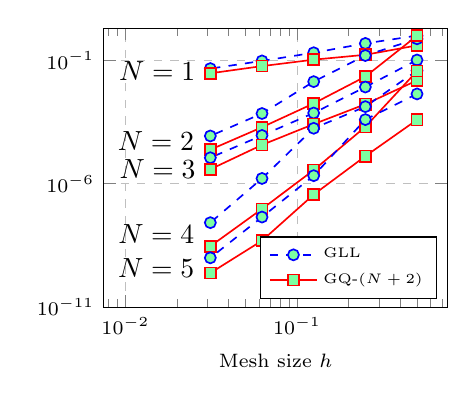
\begin{tikzpicture}
\begin{loglogaxis}[
    width=.49\textwidth,
    xlabel={Mesh size $h$},
%    ylabel={$L^2$ errors}, 
    xmin=.0075, xmax=.75,
    ymin=1e-11, ymax=2,
    legend pos=south east, legend cell align=left, legend style={font=\tiny},	
    xmajorgrids=true, ymajorgrids=true, grid style=dashed,
    legend entries={GLL,GQ-$(N+2)$}    
]
\pgfplotsset{
cycle list={{blue, dashed, mark=*}, {red, mark=square*}}
}
%\addlegendimage{no markers,blue}
%\addlegendimage{no markers,red}

\addplot+[semithick, mark options={solid, fill=markercolor}]
% N = 1, tau = 0.000000 =======================
coordinates{(0.5,1)(0.25,0.485059)(0.125,0.203599)(0.0625,0.0947163)(0.03125,0.0463705)};
\addplot+[semithick, mark options={solid, fill=markercolor}]
%N = 1, tau = 0.000000 =======================
coordinates{(0.5,0.402314)(0.25,0.167917)(0.125,0.106574)(0.0625,0.058359)(0.03125,0.0298728)}
[yshift=1pt] node[left, pos=1.025, color=black] {$N = 1$};


\addplot+[semithick, mark options={solid, fill=markercolor}]
% N = 2, tau = 0.000000 =======================
coordinates{(0.5,0.746606)(0.25,0.156701)(0.125,0.0137392)(0.0625,0.000701926)(0.03125,8.64531e-05)};
\addplot+[semithick, mark options={solid, fill=markercolor}]
%N = 2, tau = 0.000000 =======================
coordinates{(0.5,0.993771)(0.25,0.0219437)(0.125,0.00180028)(0.0625,0.000194939)(0.03125,2.4045e-05)}
[yshift=4pt] node[left, pos=1.025, color=black] {$N = 2$};


\addplot+[semithick, mark options={solid, fill=markercolor}]
% N = 3, tau = 0.000000 =======================
coordinates{(0.5,0.103299)(0.25,0.00829887)(0.125,0.00073573)(0.0625,9.05975e-05)(0.03125,1.13596e-05)};
\addplot+[semithick, mark options={solid, fill=markercolor}]
%N = 3, tau = 0.000000 =======================
coordinates{(0.5,0.0154054)(0.25,0.00167426)(0.125,0.000260859)(0.0625,3.76182e-05)(0.03125,3.86238e-06)}
[yshift=1pt] node[left, pos=1.025, color=black] {$N = 3$};

\addplot+[semithick, mark options={solid, fill=markercolor}]
% N = 4, tau = 0.000000 =======================
coordinates{(0.5,0.0385542)(0.25,0.00133048)(0.125,0.000176663)(0.0625,1.64135e-06)(0.03125,2.66024e-08)};
\addplot+[semithick, mark options={solid, fill=markercolor}]
%N = 4, tau = 0.000000 =======================
coordinates{(0.5,0.0367592)(0.25,0.000202817)(0.125,3.57758e-06)(0.0625,9.58294e-08)(0.03125,2.94985e-09)}[yshift=6pt] node[left, pos=1.025, color=black] {$N = 4$};

\addplot+[semithick, mark options={solid, fill=markercolor}]
% N = 5, tau = 0.000000 =======================
coordinates{(0.5,0.00436131)(0.25,0.00039846)(0.125,2.1282e-06)(0.0625,4.49046e-08)(0.03125,9.99912e-10)};
\addplot+[semithick, mark options={solid, fill=markercolor}]
%N = 5, tau = 0.000000 =======================
coordinates{(0.5,0.000390565)(0.25,1.31188e-05)(0.125,3.6544e-07)(0.0625,4.95271e-09)(0.03125,2.42763e-10)}
[yshift=3pt] node[left, pos=1.025, color=black] {$N = 5$};

%\legend{$N=1$,$N=2$,$N=3$,$N=4$,$N=5$}
\end{loglogaxis}
\end{tikzpicture}
}
\subfloat[With Lax-Friedrichs penalization]{
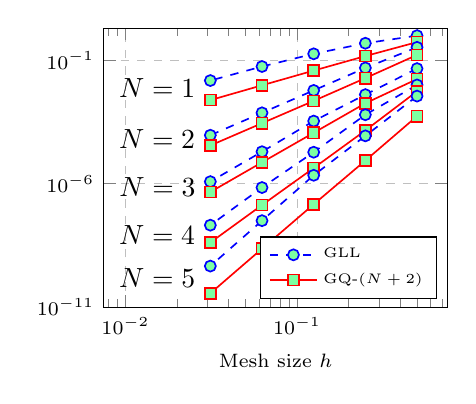
\begin{tikzpicture}
\begin{loglogaxis}[
    width=.49\textwidth,
    xlabel={Mesh size $h$},  %ylabel={$L^2$ errors}, 
    xmin=.0075, xmax=.75,
    ymin=1e-11, ymax=2,
    legend pos=south east, legend cell align=left, legend style={font=\tiny},	
    xmajorgrids=true, ymajorgrids=true, grid style=dashed,
    legend entries={GLL,GQ-$(N+2)$}
] 
\pgfplotsset{
cycle list={{blue, dashed, mark=*}, {red, mark=square*}}
}
%\pgfplotsset{cycle list={{blue, dashed, mark=*}, {red, mark=square*}}}

\addplot+[semithick, mark options={solid, fill=markercolor}]
% N = 1, tau = 0.500000 =======================
coordinates{(0.5,1)(0.25,0.4932)(0.125,0.183839)(0.0625,0.0562398)(0.03125,0.0151873)};
\addplot+[semithick, mark options={solid, fill=markercolor}]
%N = 1, tau = 0.500000 =======================
coordinates{(0.5,0.547558)(0.25,0.148981)(0.125,0.0384647)(0.0625,0.00974763)(0.03125,0.00244539)}
[yshift=5pt] node[left, pos=1.025, color=black] {$N = 1$};

\addplot+[semithick, mark options={solid, fill=markercolor}]	
% N = 2, tau = 0.500000 =======================
coordinates{(0.5,0.336817)(0.25,0.04941)(0.125,0.00605428)(0.0625,0.000748842)(0.03125,9.25456e-05)};
\addplot+[semithick, mark options={solid, fill=markercolor}]
%N = 2, tau = 0.500000 =======================
coordinates{(0.5,0.165807)(0.25,0.0190013)(0.125,0.00227903)(0.0625,0.00028425)(0.03125,3.54865e-05)}
[yshift=3pt] node[left, pos=1.025, color=black] {$N = 2$};


% N = 3, tau = 0.500000 =======================
\addplot+[semithick, mark options={solid, fill=markercolor}]
coordinates{(0.5,0.0463242)(0.25,0.00408748)(0.125,0.000346831)(0.0625,1.99064e-05)(0.03125,1.22357e-06)};
\addplot+[semithick, mark options={solid, fill=markercolor}]
%N = 3, tau = 0.500000 =======================
coordinates{(0.5,0.0174194)(0.25,0.00182234)(0.125,0.000116147)(0.0625,7.39839e-06)(0.03125,4.6305e-07)}
[yshift=3pt] node[left, pos=1.025, color=black] {$N = 3$};

\addplot+[semithick, mark options={solid, fill=markercolor}]
% N = 4, tau = 0.500000 =======================
coordinates{(0.5,0.0100716)(0.25,0.000625923)(0.125,1.89866e-05)(0.0625,7.03865e-07)(0.03125,2.10265e-08)};
\addplot+[semithick, mark options={solid, fill=markercolor}]
%N = 4, tau = 0.500000 =======================
coordinates{(0.5,0.00556743)(0.25,0.000144595)(0.125,4.33972e-06)(0.0625,1.37151e-07)(0.03125,4.16335e-09)}
[yshift=4pt] node[left, pos=1.025, color=black] {$N = 4$};


\addplot+[semithick, mark options={solid, fill=markercolor}]
% N = 5, tau = 0.500000 =======================
coordinates{(0.5,0.00356628)(0.25,8.73125e-05)(0.125,2.20528e-06)(0.0625,3.20127e-08)(0.03125,4.63639e-10)};
\addplot+[semithick, mark options={solid, fill=markercolor}]
%N = 5, tau = 0.500000 =======================
coordinates{(0.5,0.000547621)(0.25,8.7194e-06)(0.125,1.47105e-07)(0.0625,2.34345e-09)(0.03125,3.65306e-11)}
[yshift=7pt] node[left, pos=1.025, color=black] {$N = 5$};

\end{loglogaxis}
\end{tikzpicture}
}
%\caption*{$L^2$ errors under mesh refinement for entropy conservative and Lax-Friedrichs fluxes under both Gauss-Legendre-Lobatto (GLL) and over-integrated $(N+2)$ point Gauss quadrature (GQ-$(N+2)$).}
\label{fig:convergence}
\end{figure}
}

\frame[noframenumbering]{
\frametitle{Conservation of entropy: semi-discrete vs.\ fully discrete}
\setcounter{subfigure}{0}

\vspace{-1em}
%\begin{itemize}
%\item Entropy conservation: \textit{semi-discrete}, not fully discrete.
\begin{center}
\item $\Delta S(\bm{u}) = \LRb{S(\bm{u}(x,t))-S(\bm{u}(x,0))} \rightarrow 0$ as as $\Delta t \rightarrow 0$.
\end{center}
%\end{itemize}
\vspace{-.5em}
\begin{figure}
\centering
\subfloat[$\Delta S(\bm{u})$ for various $\Delta t$]{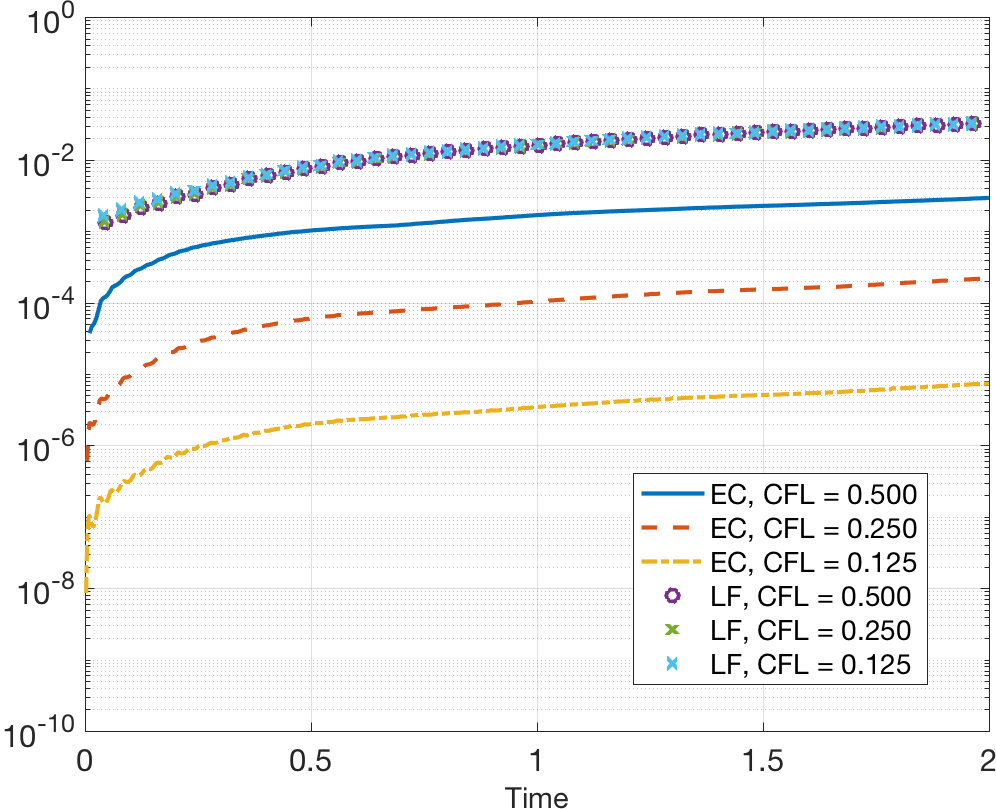
\includegraphics[width=.445\textwidth]{figs/dS_ECLF.png}}
\hspace{1em}
\subfloat[$\rho(x), u(x)$ ($N=4, K = 16$)]{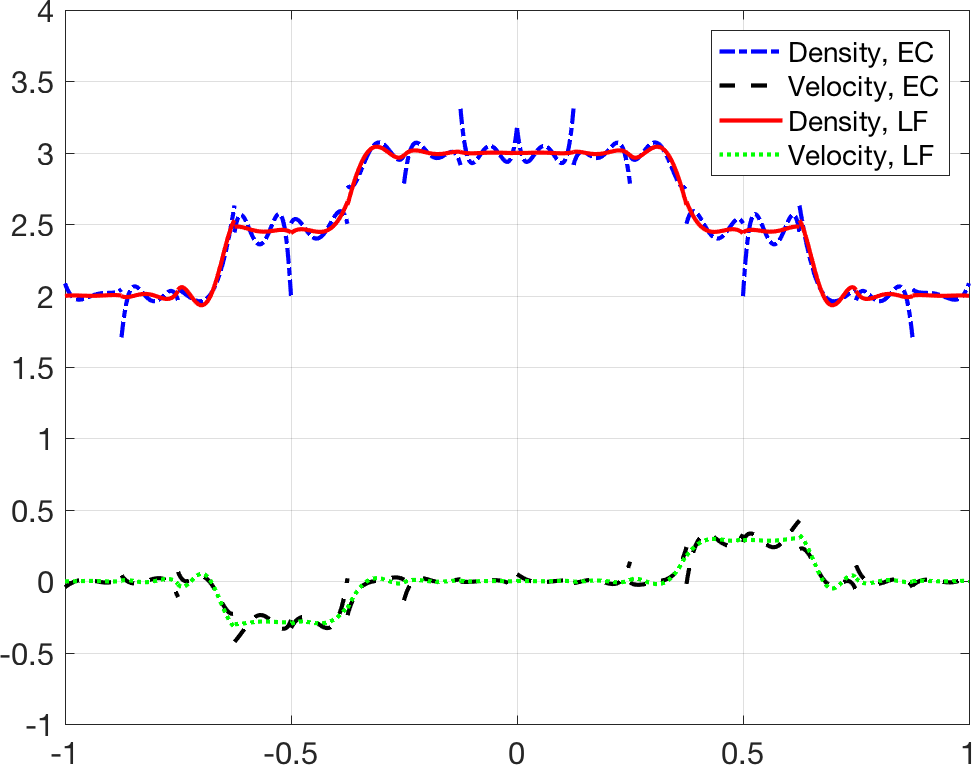
\includegraphics[width=.46\textwidth]{figs/sol_ECLF.png}}
\caption*{Solution and change in entropy $\Delta S(\bm{u})$ for entropy conservative (EC) and Lax-Friedrichs (LF) fluxes (using GQ-$(N+2)$ quadrature). }
\end{figure}
}

%\frame{
%\frametitle{1D Sod shock tube}
%
%\begin{itemize}
%\item Circles are cell averages, CFL of .125, LSRK-45 time-stepping.  
%%\item CFL of .125 used for both GLL-$(N+1)$and GQ-$(N+2)$.
%\item Comparison between $(N+1)$-point Lobatto and $(N+2)$-point Gauss.
%\end{itemize}
%\begin{figure}
%\centering
%\only<1>{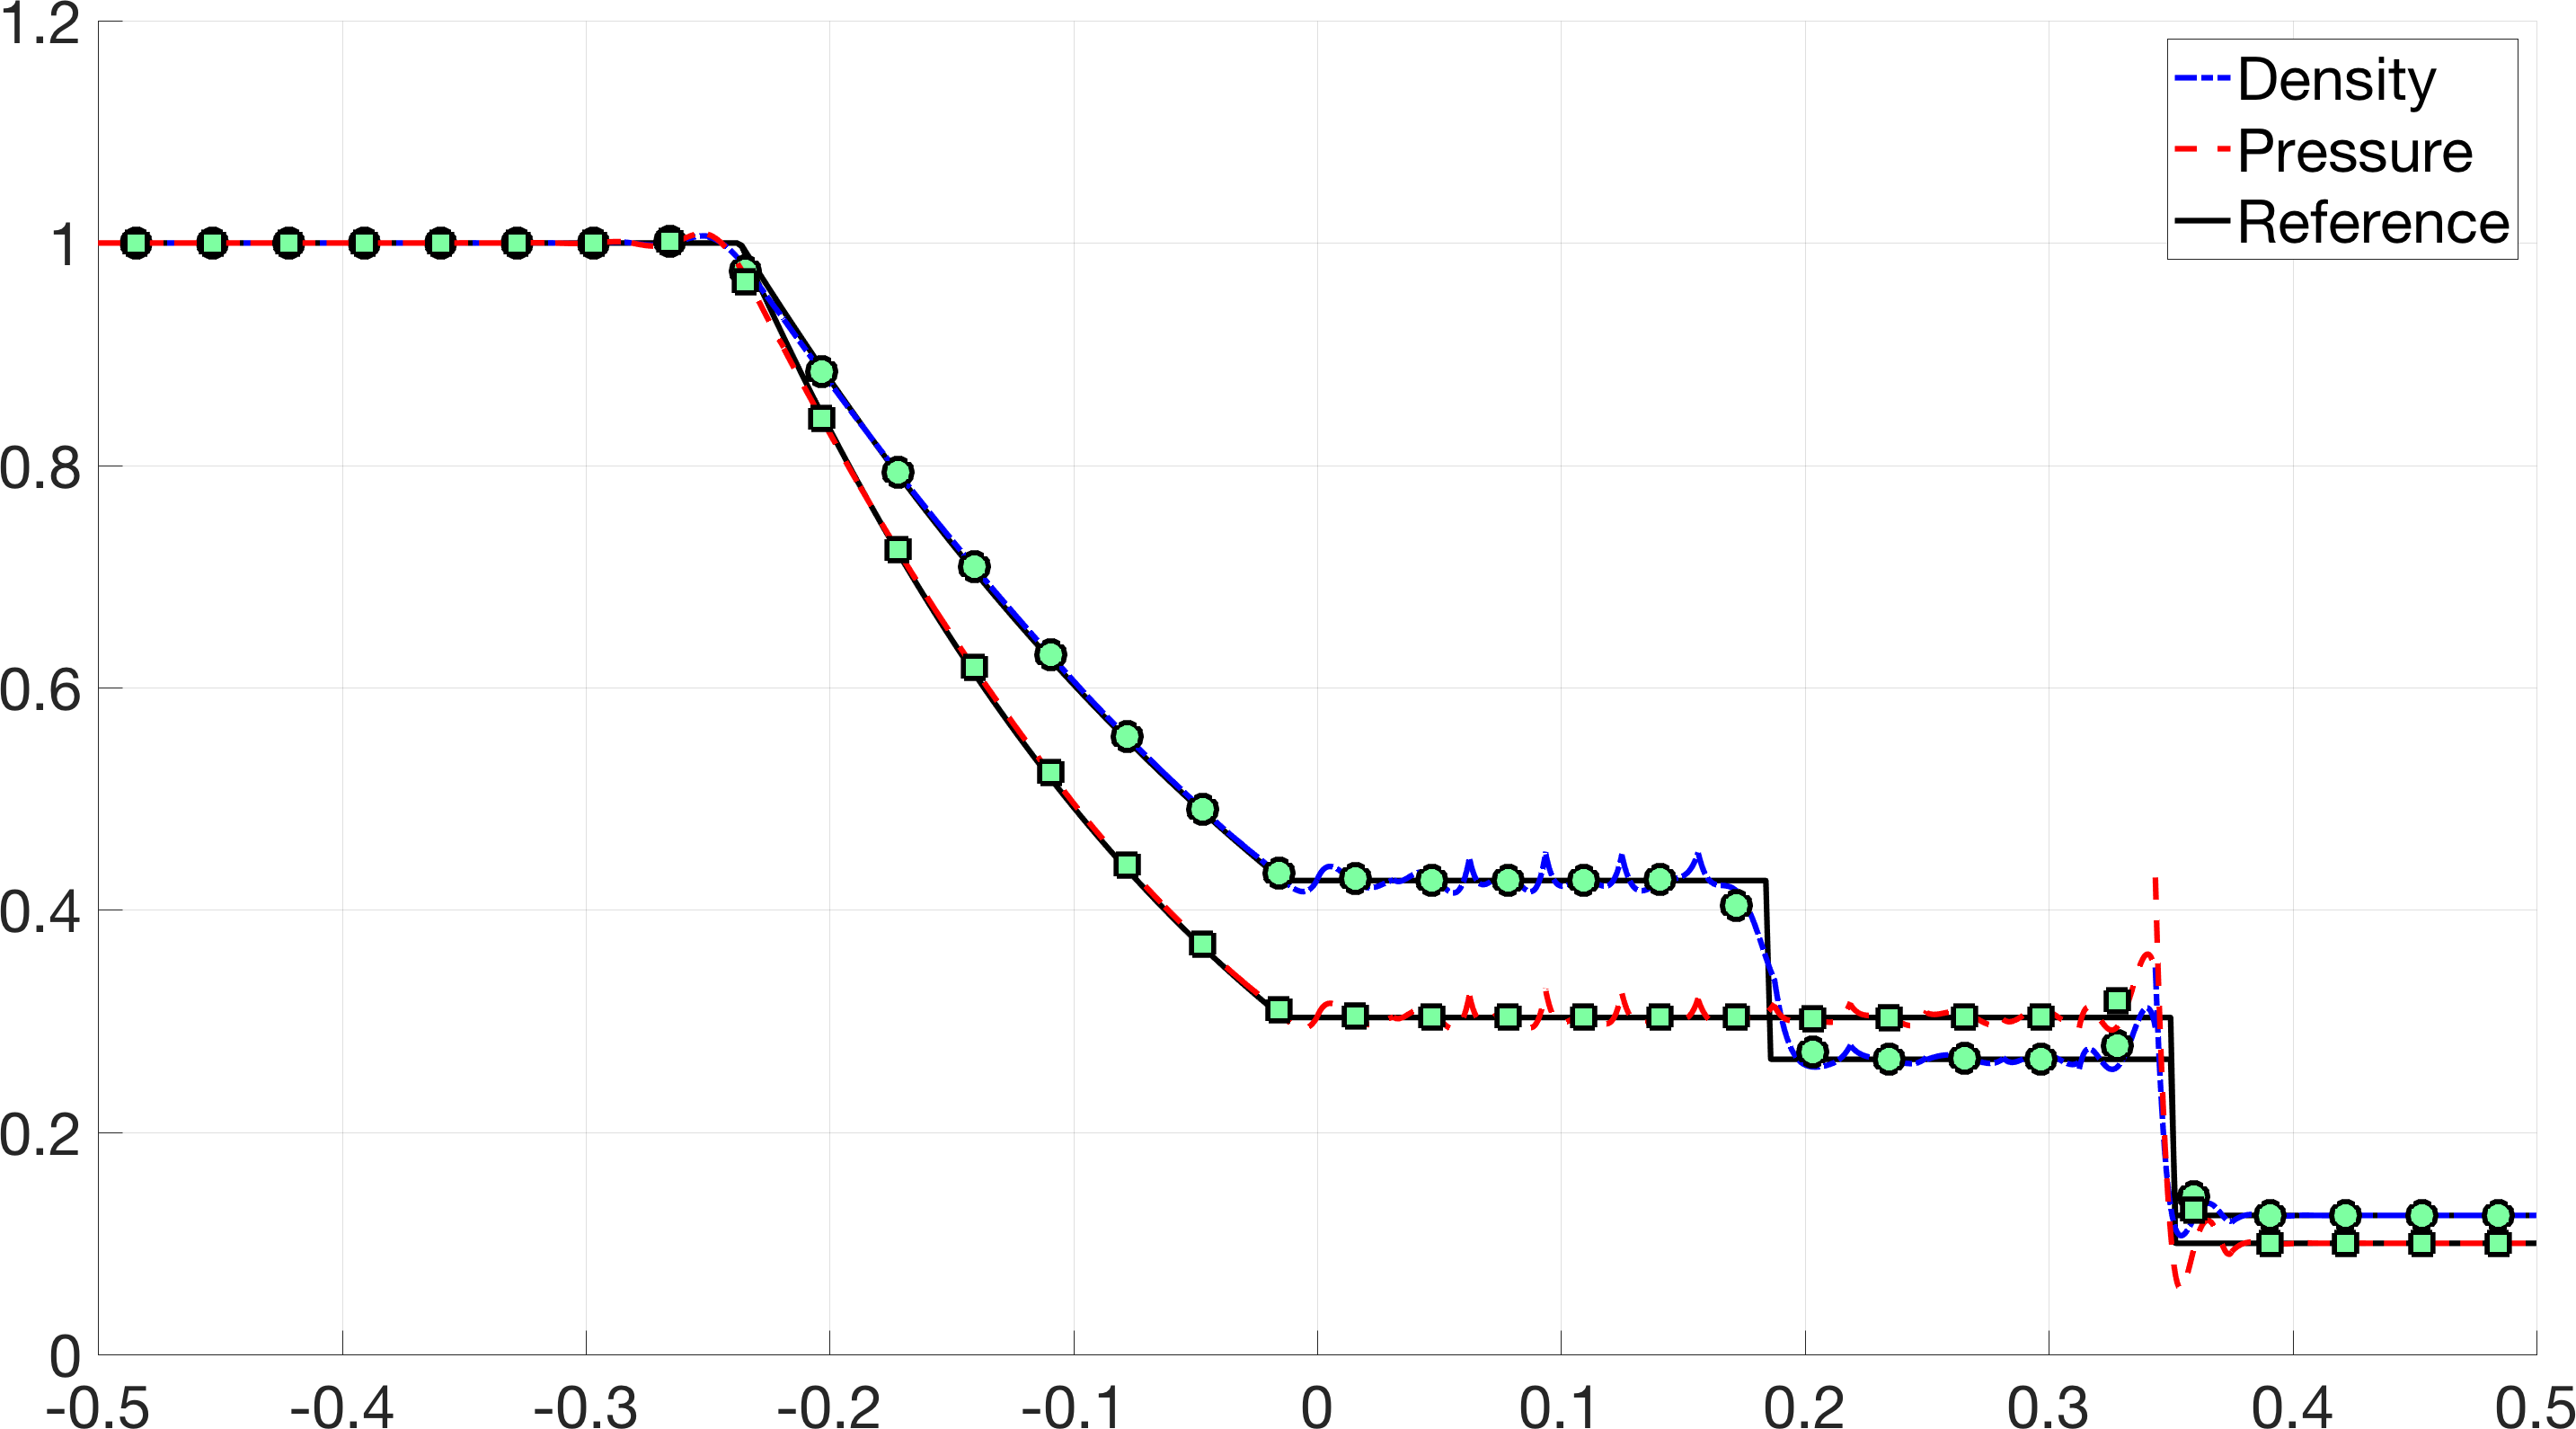
\includegraphics[width=.8\textwidth]{figs/sodGLL.png}\caption*{$N=4, K = 32$, $(N+1)$ point Lobatto quadrature.}}
%\only<2>{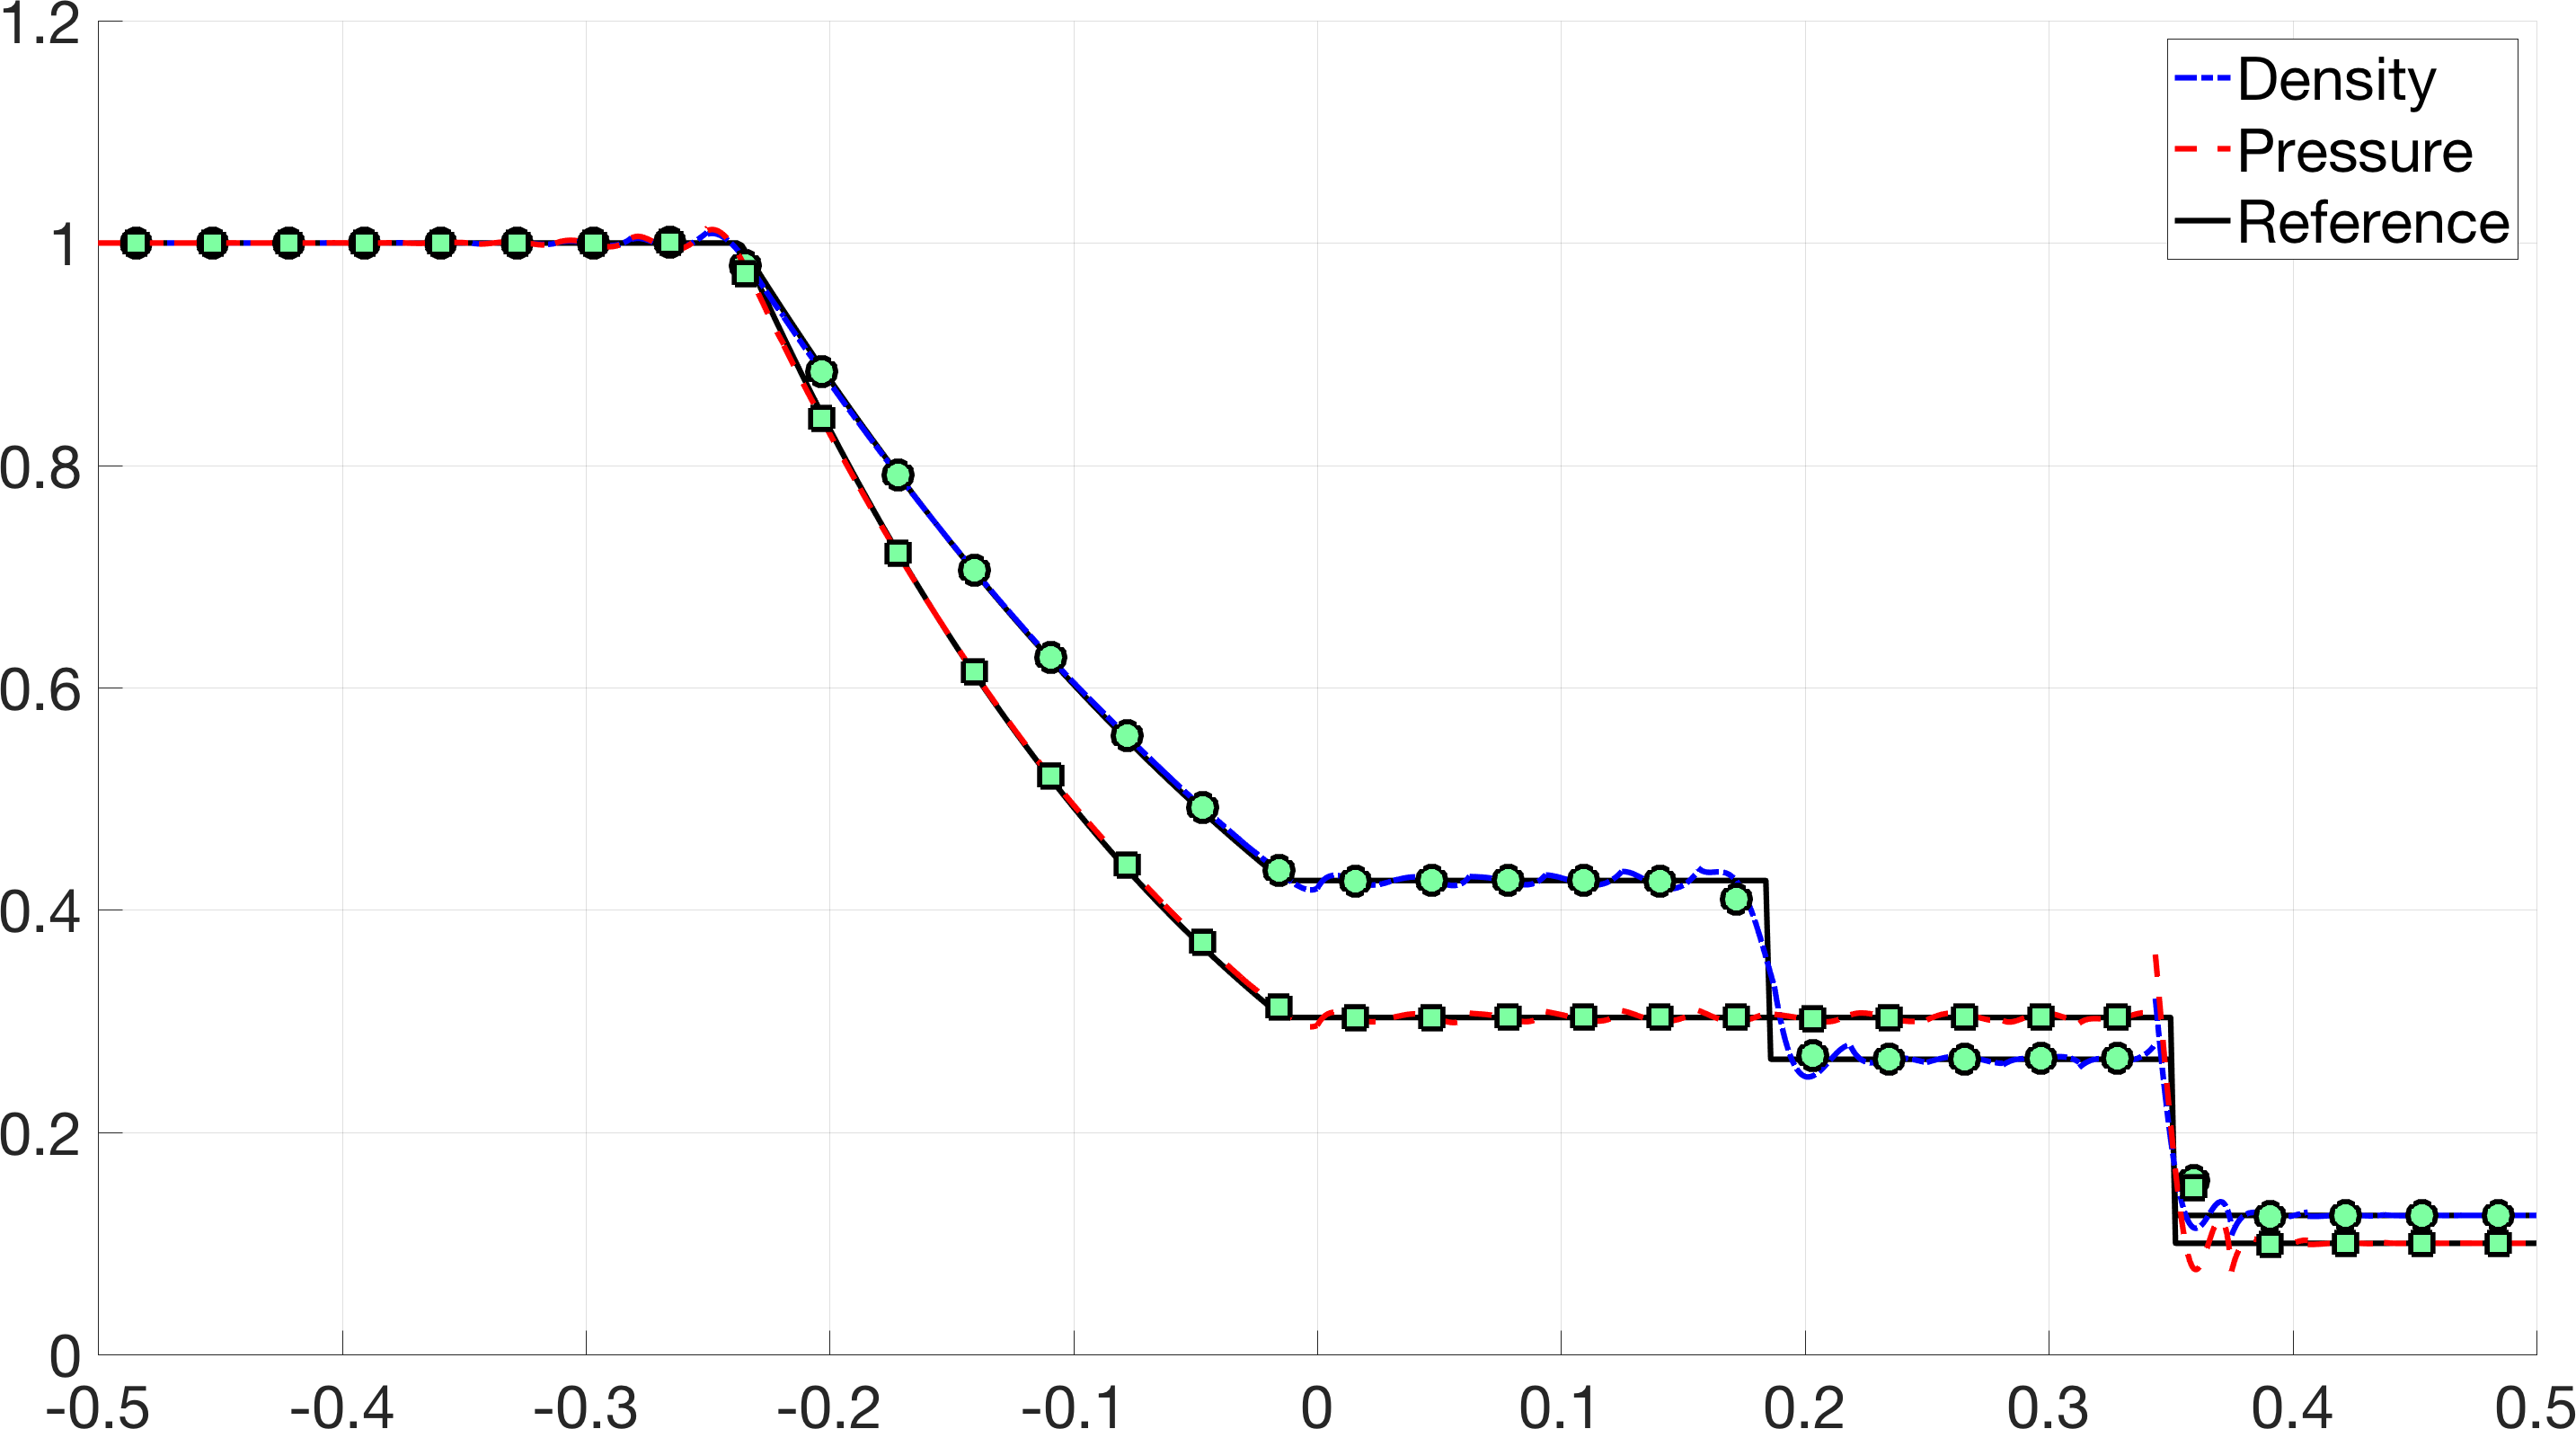
\includegraphics[width=.8\textwidth]{figs/sodGQ2.png}\caption*{$N=4, K = 32$, $(N+2)$ point Gauss quadrature.}}
%\end{figure}
%}

\frame[noframenumbering]{
\frametitle{1D sine-shock interaction}

\begin{itemize}
\item $(N+2)$-point Gauss needs a smaller CFL (.05 vs .125) for stability.  
\end{itemize}

\begin{figure}
\centering
\only<1>{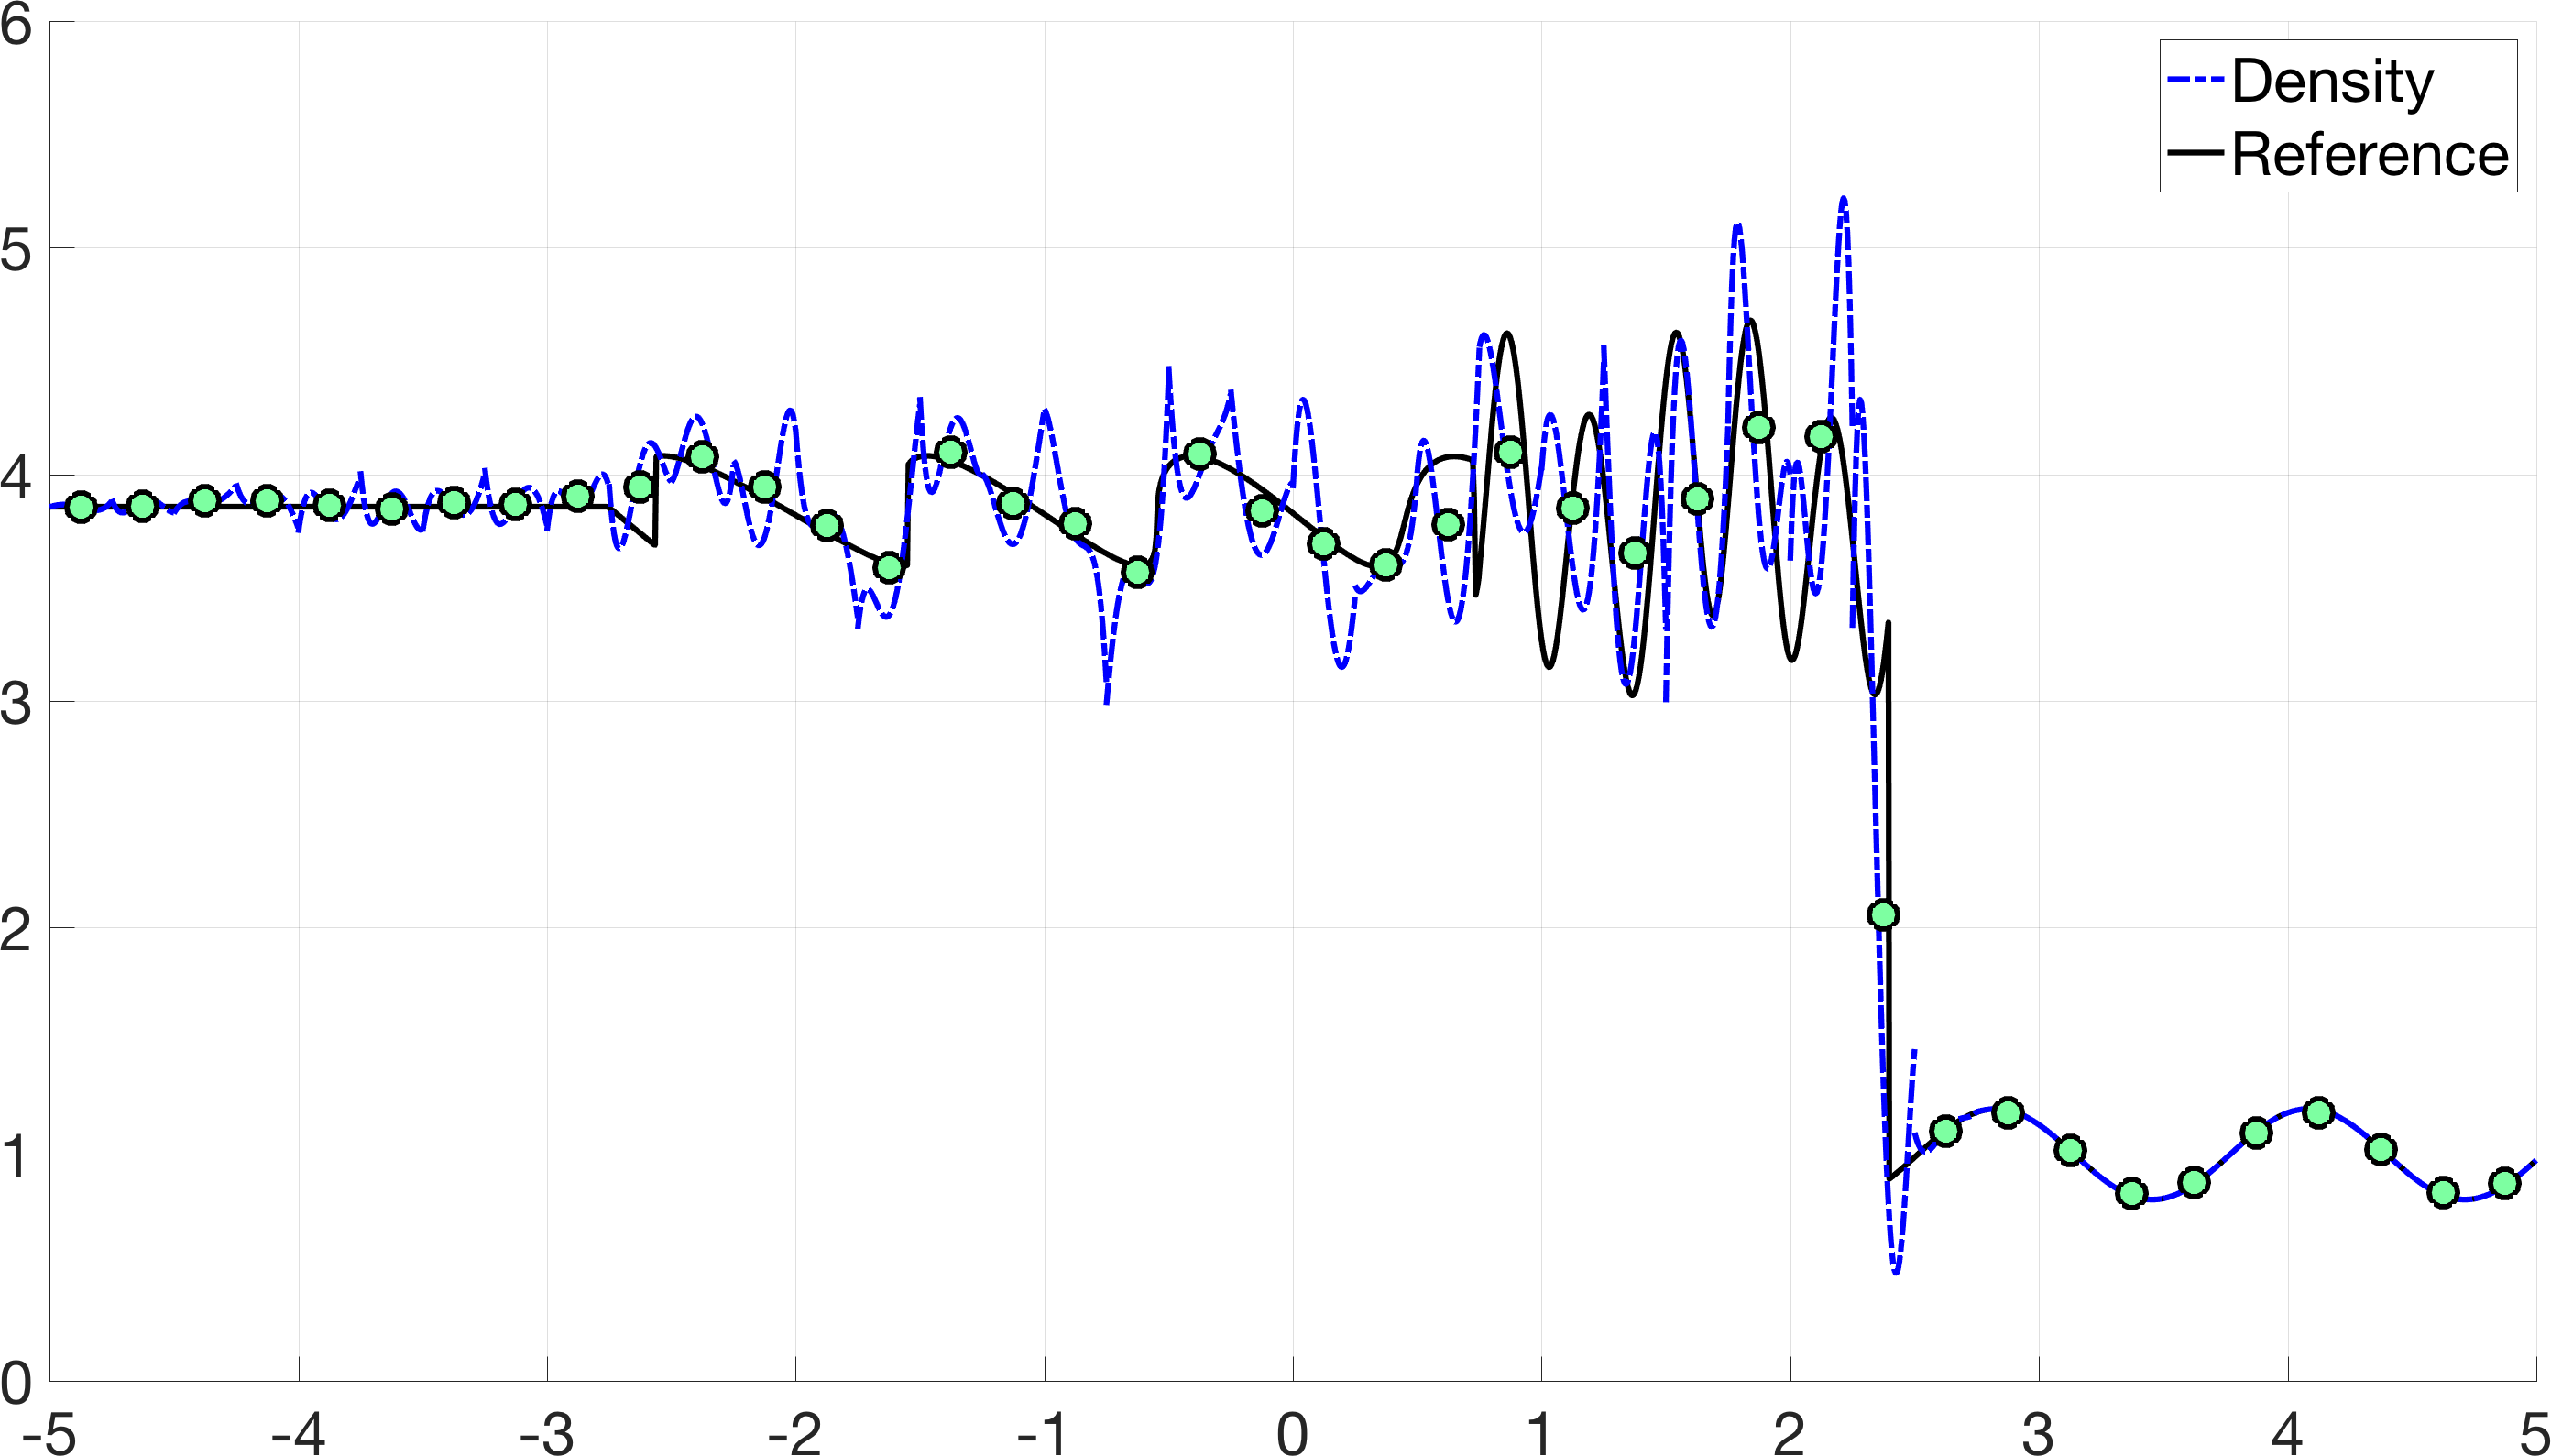
\includegraphics[width=.8\textwidth]{figs/sineShockGLL.png}\caption*{$N=4, K = 40, CFL = .05$, $(N+1)$ point Lobatto quadrature.}}
\only<2>{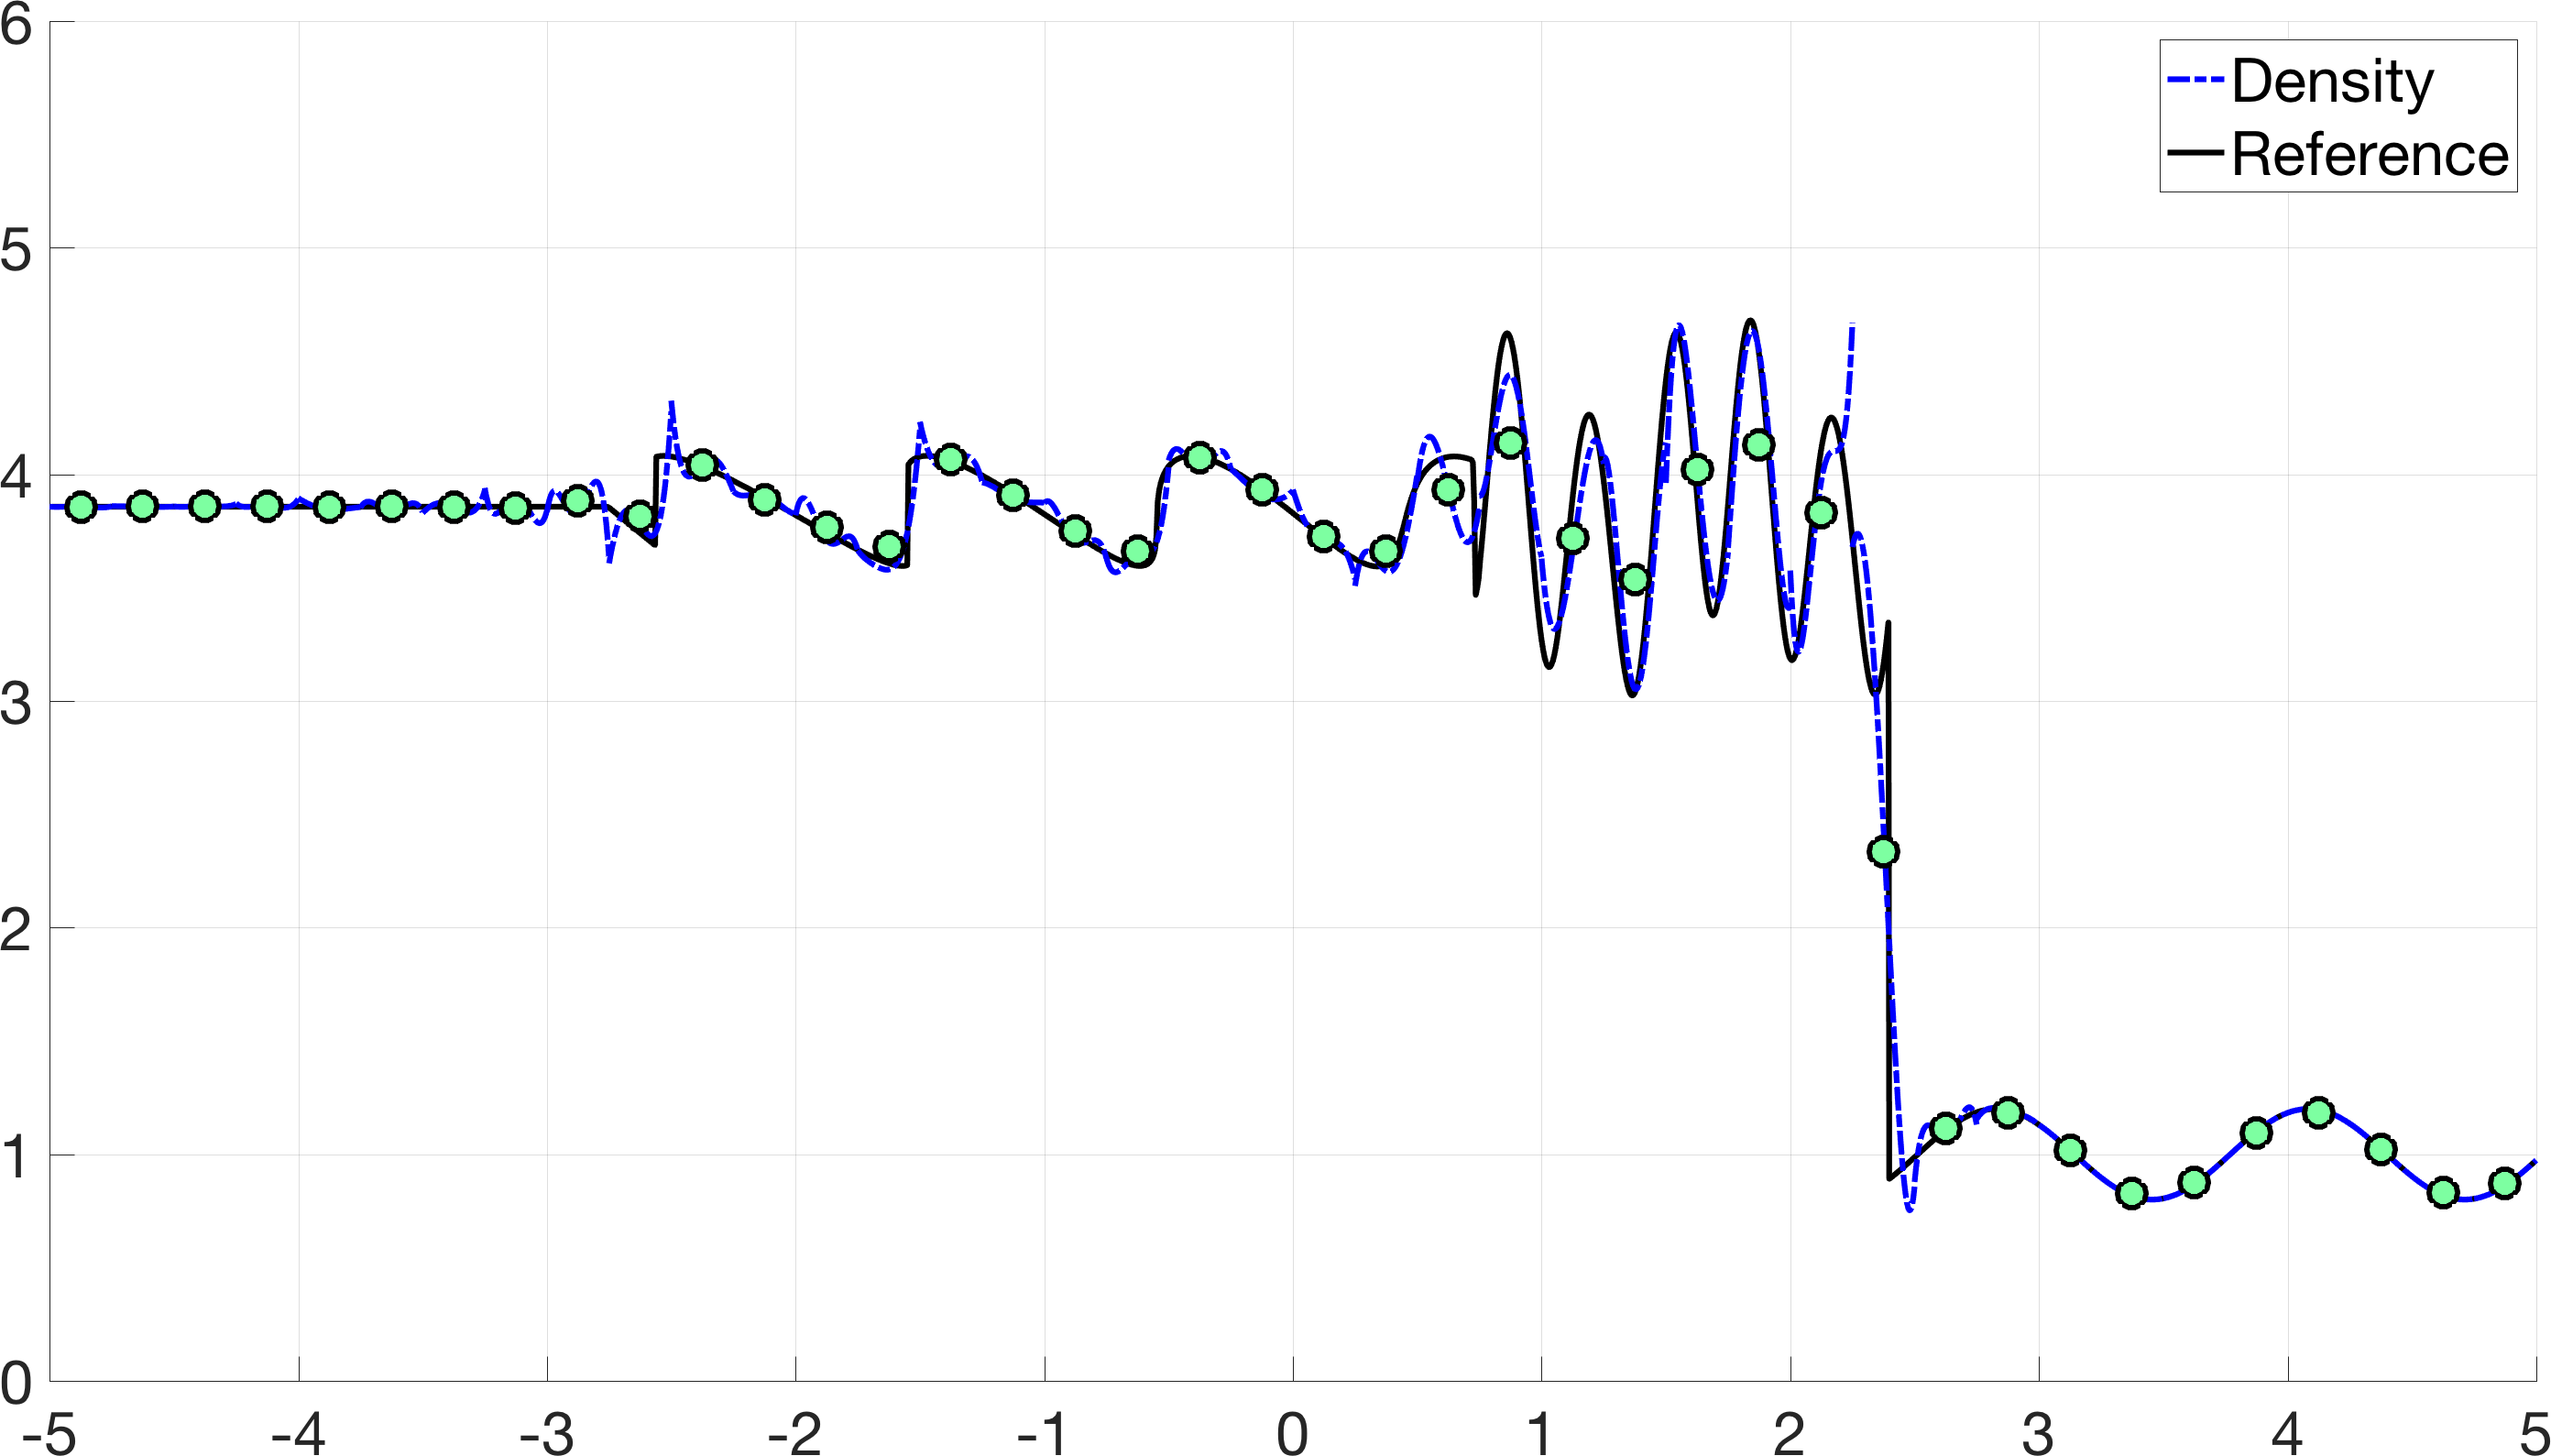
\includegraphics[width=.8\textwidth]{figs/sineShockGQ2.png}\caption*{$N=4, K = 40, CFL = .05$, $(N+2)$ point Gauss quadrature.}}
\end{figure}
}

\frame[noframenumbering]{
\frametitle{Loss of control with the entropy projection}

\begin{itemize}
\item For $(N+1)$-Lobatto quadrature, $\tilde{\bm{u}} = \bm{u}\LRp{P_N \bm{v}} = \bm{u}$ at nodal points.
\item For $(N+2)$-Gauss, discrepancy between $\bm{v}(\bm{u})$ and $L^2$ projection.
\item Still need \note{positivity} of thermodynamic quantities for stability!
\end{itemize}
\vspace{-1em}
\begin{figure}
\centering
\subfloat[${v}_3(x), \LRp{P_N v_3}(x)$]{\includegraphics[width=.45\textwidth]{figs/sineShockQ3Compare.png}}
\hspace{1em}
\subfloat[$\rho(x), \rho\LRp{\LRp{P_N \bm{v}}(x)}$]{\includegraphics[width=.44\textwidth]{figs/sineShockDensityCompare.png}}
\end{figure}
}

\frame[noframenumbering]{
\frametitle{Over-integration is ineffective without $L^2$ projection}

\begin{figure}[!h]
\centering
\begingroup
\captionsetup[subfigure]{width=.5\textwidth}
\subfloat[$(N+1)$ points]{\includegraphics[width=.45\textwidth]{figs/sbpGLL.png}}
\hspace{1em}
\subfloat[$(N+4)$ points]{\includegraphics[width=.45\textwidth]{figs/sbpGLLNp4.png}}
\endgroup
\caption{Numerical results for the Sod shock tube for $N=4$ and $K=32$ elements.  Over-integrating by increasing the number of quadrature points does not improve solution quality.  }
\label{fig:sbpq}
\end{figure}
}

\frame[noframenumbering]{
\frametitle{2D Riemann problem}
\setcounter{subfigure}{0}

\begin{itemize}
\item Uniform $64\times 64$ mesh: $N=3$, CFL $.125$, Lax-Friedrichs stabilization.
\item No limiting or artificial viscosity required to maintain stability!
\item Periodic on larger domain (``natural'' boundary conditions unstable).
\end{itemize}
\vspace{-1em}
\begin{figure}
\centering
\subfloat[$\Omega = \LRs{-1,1}^2$]{\includegraphics[width=.425\textwidth]{figs/riemannBig.png}}
\hspace{2em}
\subfloat[$\Omega =\LRs{-.5,.5}^2$, $32\times 32$ elements]{\includegraphics[width=.425\textwidth]{figs/riemannSmall.png}}
\end{figure}
}



\frame[noframenumbering]{
\frametitle{Non-conforming interfaces and SBP mortars} 
\vspace{-1em}
%\begin{columns}
%\column{0.475\textwidth}
\begin{figure}
\centering
\subfloat{\includegraphics[width=.45\textwidth]{figs/mortar.png}}
\hspace{1em}
\subfloat{\includegraphics[width=.45\textwidth]{figs/mortar_coupling.png}}
%\begin{overlayarea}{\textwidth}{.375\textheight}
%\only<1-4>{\includegraphics[width=\textwidth]{figs/mortar.png}}
%\only<5->{\includegraphics[width=\textwidth]{figs/mortar_coupling.png}}
%%\subfloat[Mortar coupling]{\includegraphics[width=.425\textwidth]{figs/mortar_coupling.png}}
%\end{overlayarea}
\end{figure}

%\column{0.475\textwidth}
%%\setlength\arraycolsep{2em}
%\only<1>{
%\[
%\underbrace{\begin{bmatrix}
%\bm{Q}_i-\bm{Q}_i^T & \bm{E}^T\bm{B}_i &\\
%-\bm{B}_i\bm{E} &  
%\end{bmatrix}}_{\text{skew operator } \bm{Q}^i_N- \LRp{\bm{Q}^i_N}^T}
%\]
%}
%\only<2->{
%\[
%\underbrace{\begin{bmatrix}
%\bm{Q}_i-\bm{Q}_i^T & \bm{E}^T\bm{B}_i &\\
%-\bm{B}_i\bm{E} &  & \bm{B}_i\tilde{\bm{E}}_m \\
%& -\tilde{\bm{B}}_i{\bm{E}}_m & 
%\end{bmatrix}}_{\text{modified skew operator } \bm{Q}^i_N- \LRp{\bm{Q}^i_N}^T}
%\]
%}
%\end{columns}

\begin{itemize}
\item Define appropriate interpolation operators $\bm{E}_m, \tilde{\bm{E}}_m$ between conforming and non-conforming (mortar) nodes.
\item \only<1-2>{Modify the skew-symmetric formulation as follows:} \only<3->{Rewrite as modification of numerical flux.}
%\vspace{-1em}
\begin{overlayarea}{\textwidth}{.25\textheight}
\only<1>{
\[
\bm{M}\td{\bm{u}}{t} + \sum_{i=1}^d\begin{bmatrix}
\bm{V}_q\\
\bm{V}_f
\end{bmatrix}^T
\begin{bmatrix}
\bm{Q}_i-\bm{Q}_i^T & \bm{E}^T\bm{B}_i \\
-\bm{B}_i\bm{E} &  
\end{bmatrix}
+ \bm{E}^T\bm{B}_i\bm{f}_i^* = 0.
\]
}
\only<2>{
%\vspace{-.5em}
\[
\hspace*{-3em}\bm{M}\td{\bm{u}}{t} + \sum_{i=1}^d\begin{bmatrix}
\bm{V}_q\\
\bm{V}_f\\
\note{\bm{V}_m}
\end{bmatrix}^T
\begin{bmatrix}
\bm{Q}_i-\bm{Q}_i^T & \bm{E}^T\bm{B}_i &\\
-\bm{B}_i\bm{E} &  & \note{\bm{B}_i\tilde{\bm{E}}_m} \\
& \note{-\tilde{\bm{B}}_i{\bm{E}}_m} & 
\end{bmatrix}
+ \note{\bm{V}_m}^T \tilde{\bm{B}}_i{\bm{f}}_i^* = 0.
\]
}
\only<3->{
%\vspace{-1em}
\begin{align*}
%\bm{M}\td{\bm{u}}{t} &+ \sum_{i=1}^d
%\begin{bmatrix} 
%\bm{V}_q\\
%\bm{V}_f
%\end{bmatrix}^T
%\LRp{\begin{bmatrix}
%\bm{Q}_i-\bm{Q}_i^T & \bm{E}^T\bm{B}_i\\
%-\bm{B}_i\bm{E} & \\
%\end{bmatrix} \circ \bm{F}_S}\bm{1} + \bm{V}_f^T\bm{B}_i \tilde{\bm{f}}^*_i = 0\\
\tilde{\bm{f}}^*_i &= \tilde{\bm{E}}_m\bm{f}^*_i + \LRp{\tilde{\bm{E}}_m\circ \bm{F}_S^{sm}}\bm{1} - \tilde{\bm{E}}_m \LRp{ \bm{E}_m \circ \bm{F}_S^{ms}}\bm{1} 
\end{align*}
}
\end{overlayarea}
\end{itemize}
}


\bibliographystyle{plain}
{\scriptsize
\bibliography{pyramids}
}

\end{document}
